\chapter{Introducción a la optimización convexa}

\columnratio{0.7,0.3}
\begin{paracol}{2}
\section{Introducción}

\begin{tcolorbox}[colback=black!1!white,colframe=white!90!black]
$$
(P)
\left\{
\begin{array}{rl}
    \min & f_0(x)\\\\
    s.a. & f_1(x) \leq b_1\\
	 &f_2(x) \leq b_2\\
	 & \vdots\\
	 & f_m(x) \leq b_m.
\end{array}
\right.
$$
\end{tcolorbox}

Donde,
\switchcolumn[1]*{\noindent \scriptsize
    \begin{itemize}
	\item Las funciones objetivos en economía se les puede llamar funciones de coste.
	\item Multiplicamos las desigualdades por $(-1)$ para darle la forma que más nos convenga darle al problema de optimización.
	\item Maximizar será lo mismo que minimizar. En nuestro caso minimizaremos las funciones. 
	\item Al valor $f_0(x^*)$ se le llamará valor optimo.
	\item En $f_i:  \mathbb{R}^n \rightarrow \mathbb{R}$ existirán algunas funciones el cual su dominio sera "tramposo".
    \end{itemize}
}

\switchcolumn[0]
$$
\begin{array}{rl}
    f_i: & \mathbb{R}^n \rightarrow \mathbb{R}\\
    f_0 : & \mbox{Función objetivo.}\\
    f_j : & \mbox{Función Restricción donde }j=1,\ldots,m.\\
\end{array}
$$

El objetivo de (P) es encontrar $x^*$ el optimo ($\arg\min$) que cumpla:

	    $$f_0(x^*)\leq f_0(x), \;\forall x\in \mathbb{R}^n / f_j(x)\leq b_j,\; j=1,\ldots,m.$$

Los Puntos factibles son los $x\in \mathbb{R}^n / f_j(x)\leq b_j,\; j=1,\ldots,m.$\\

Cuando el problema sea de la forma convexa se llama optimización convexa. Al final, la habilidad es identificar las restricciones y convertirlas a convexas.

\switchcolumn[1]*{\scriptsize
% -------------------- NOTA 1.1
\begin{nota} Imaginemos que tenemos
    $$
    \begin{array}{rl}
	\left\{\min\right. & f(x)\\\\
	\left\{ \min \right. & f_0^2(x)
    \end{array}
    $$
    \begin{itemize}
	\item Si las función $f_0$ es positiva las dos formas son equivalentes. 
	\item El valor optimo no será el mismo, pero el punto optimo lo será, ya que las funciones son monótomas crecientes. 
	\item Si el valor al cuadrado simplificará la solución, entonces podemos utilizarla. Esto nos permite que si no tengamos una función convexa podamos convexificarla.
    \end{itemize}
\end{nota}
}
\switchcolumn[0]\noindent
% -------------------- NOTACIÓN 1.1
\begin{notacion}
    Podemos escribir $Ax$ como
    $$
    \begin{array}{rcl}
	Ax &=& 
	\underset{A^1}{
	\begin{pmatrix}
	    a_{11}\\
	    a_{21}\\
	    \vdots\\
	    a_{k1}
	\end{pmatrix}}
	x_1+
	\underset{A^2}{
	\begin{pmatrix}
		a_{12}\\
		a_{22}\\
		\vdots\\
		a_{k2}
	\end{pmatrix}}
	x_2+
	\cdots +
	\underset{A^n}{
	\begin{pmatrix}
		a_{1n}\\
		a_{2n}\\
		\vdots\\
		a_{kn}
	\end{pmatrix}}
	x_n\\\\
       &=&
	x_1A^1+x_2A^2+\cdots+x_nA^n.
    \end{array}
    $$
    $A^1$ = A super 1 como columna, y $A_1$ = A super 1 como fila.\\

    Ahora, en términos de filas. Si escribimos los vectores A en columna
    $$
    A = 
    \begin{pmatrix}
	    A^T_1\\
	    A^T_2\\
	    \vdots\\
	    A^T_k
    \end{pmatrix}
    $$

    Donde,\\
    $$
    Ax = 
    \begin{pmatrix}
	    A^T_1x\\
	    A^T_2x\\
	    \vdots\\
	    A^T_nx
    \end{pmatrix}
    =
    \begin{pmatrix}
	    \langle A^T_1,x\rangle\\
	    \langle A^T_2,x\rangle\\
	    \vdots\\
	    \langle A^T_n,x\rangle
    \end{pmatrix}
    $$
\end{notacion}


% -------------------- EJEMPLO 1.1 -----------------------------
\begin{ejem}
    Sean $A\in \mathcal{M}_{k\times n},\; \textbf{x}\in \mathbb{R}^n,\; \textbf{b}\in \mathcal{R}^k$.
    $$
    \begin{pmatrix}
	x_1\\
	x_2\\
	\vdots\\
	x_n
    \end{pmatrix}
    \in \mathbb{R}^n,
    \qquad 
    \textbf{x}^T=(x_1,x_2,\ldots,x_n).
    $$
    El problema será una minimización global dada por:\;
    $
    \left\{
    \begin{array}{rl}
	\min: &\|A\textbf{x}-b\|^2_2\\
	s.a. & \emptyset.
    \end{array}
    \right.
    $
\switchcolumn[1]*{\noindent \scriptsize
    \begin{itemize}
	\item Diremos que el un vector cualquiera sera vector columna.
	\item El subindice $_2$ significa la normal Euclidea. Que es la distancia normal que existe en $\mathbb{R}^2.$
    \end{itemize}
}

\switchcolumn[0]
    Solución.-\; Por diferenciabilidad se tiene,
    $$f_0(x)=\|Ax-b\|_2^2 = \langle Ax-b,Ax-b\rangle.$$
    Intentaremos demostrar el punto donde las parciales de $f_0=0$. Para ello, encontraremos 
    $$
    \begin{array}{rcl}
	D_if_0&=&D_i\left(\langle Ax-b, Ax-b\rangle\right)\\\\
	      &=&\langle D_i\left(Ax-b\right),Ax-b\rangle+\langle Ax-b,D_i\left(Ax-b\right)\rangle\\\\
	      &=& 2\langle Ax-b,D_i\left(Ax-b\right)\rangle.
    \end{array}
    $$
    Veamos la parcial de $D_i\left(Ax-b\right)$.
    $$ D_i\left(Ax-b\right)=D_i\left(x_1A^1+x_2A^2+\cdots+x_nA^n-b\right)=A^i.$$
    Dado que $b$ que es constante vale cero, y donde todos los suman que no estén las $x_i$ también valen cero.
    Por lo tanto,
    $$D_if_0 = 2\langle Ax-b,A^i \rangle.$$
    Luego, 
    $$2\langle Ax-b,A^i \rangle = 0 \; \forall i=1,\ldots,n \quad \Rightarrow \quad \langle Ax-b,A^i\rangle=0,\quad \forall i = 1,\ldots,n.$$

\switchcolumn[1]*{\scriptsize
    \begin{itemize}
	\item En funciones convexas el extremo local será el mínimo global.
    \end{itemize}
}
\switchcolumn[0]\noindent
	Observemos que,
	$$
	\overrightarrow{0} = 
	\begin{pmatrix}
	    \langle Ax-b,A^1\rangle\\
	    \langle Ax-b,A^2\rangle\\
	    \vdots\\
	    \langle Ax-b,A^n\rangle
	\end{pmatrix}
	=
	\begin{pmatrix}
	    (A_1)^T\\
	    (A_2)^T\\
	    \vdots\\
	    (A_n)^T
	\end{pmatrix}
	(Ax-b)
	=A^T(Ax-b).
	$$
	$$A^T(Ax-b)=\overrightarrow{0}\quad \Leftrightarrow\quad A^TAx=A^Tb.$$
	El cual es una ecuación normal.

Por último, veamos los argumentos geométricos. Notemos que,
$$\min \|Ax-b\|^2_2 = d(b_i,Ax)^2$$
Donde $Ax$ tendrá la forma geométrica de un subespacio vectorial (en el caso de $\mathbb{R}^3$ será un plano). Entonces,
\switchcolumn[1]*{\noindent
\begin{center}
    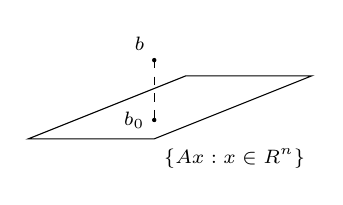
\begin{tikzpicture}[scale=0.4]
      % Define los vértices del romboide
      \coordinate (A) at (0,0);
      \coordinate (B) at (4,0);
      \coordinate (C) at (9,2);
      \coordinate (D) at (5,2);
      % Dibuja el romboide y etiqueta sus vértices
      \draw (A) -- (B) -- (C) -- (D) -- cycle;
      % Que el plano se llame P
      \node [below right] at (B) {$\left\{Ax:x\in \mathbb{R}^n\right\}$};
      % trazar una linea entrecortada perpedicular al plano y los puntos extremos que tengan un punto negro
      \draw[dashed] (4,2.5)node[above left]{$b$} -- (4,.6)node[left]{$b_0$};
      \fill (4,2.5) circle (2pt);
      \fill (4,.6) circle (2pt);
    \end{tikzpicture}
\end{center}
}
\switchcolumn[0]\noindent
    \begin{itemize}
	\item Si $b\in \left\{Ax:x\in \mathbb{R}^n\right\}\; \Leftrightarrow \; x^* \in \mathbb{R}^n : Ax^* =b.$ El valor optimo es $f_0(x^*)=0$.
	\item Si $b\notin \left\{Ax:x\in \mathbb{R}^n\right\}$, $f_0(x^*)=d(b,b_0)^2$.
    \end{itemize}
Ahora, cual es el optimo?; es decir cual es el $x^*$. Para ello, 
$$x^*\in \mathbb{R}^n : Ax^*=b_0.$$ Aquí, $b_0$ está en el plano, si estamos en $\mathbb{R}^3$. ¿Cómo llegamos algebraicamente?:
$$
\begin{array}{rcl}
b-b_0 \perp \left\{Ax:x\in \mathbb{R}^n\right\}&\Leftrightarrow & b-b_o \perp A^i,\; i=1,\ldots,n\\\\  
						 &\Leftrightarrow & \langle b-b_0,A^i\rangle=0,\; i=1,\ldots,n\\\\
							   &\Leftrightarrow& \langle b-Ax^*,A^i\rangle = 0, \; i=1,\ldots,n\\\\
							   &\Leftrightarrow& \langle Ax^*-b,A^i\rangle = 0, \; i=1,\ldots,n\\\\
								   &\Leftrightarrow&A^TAx^*=A^Tb.
\end{array}
$$
(Las ecuaciones normales vienen dadas por la perpendicularidad.)
\end{ejem}

\end{paracol}



\chapter{Conjuntos convexos}

\begin{paracol}{2}

\section{Conjuntos convexos de \boldmath $\mathbb{R}^n$}
El dominio serán conjuntos convexos o dominio efectivo.
\switchcolumn[1]*{\noindent \scriptsize
    \begin{itemize}
	\item Cuando $\lambda$ vale $1$ será $x_1$ cuando valga cero $x_0$. 
	\item Cuando es positivo irá a  la derecha, cuando es negativo hacia la izquierda.
	\item Toda la recta nos da un concepto que denominamos Afín. 
	    Es cualquier punto que este entre $x_0$ y $x_1$ del gráfico de arriba. 
    \end{itemize}
}
\switchcolumn[0]\noindent
    % -------------------- DEFINICIÓN 1 LINEAL
    \begin{def.}[Lineal]\,\\ 
    $$L(x_0,x_1) := \left\{x_0+\lambda(x_1-x_0):\lambda \in \mathbb{R}\right\}$$
    \begin{center}
	\begin{tikzpicture}[scale=0.35]
	  \coordinate (A) at (0,0);
	  \coordinate (B) at (3,1);
	  \coordinate (C) at (6,2);
	  \coordinate (D) at (-3,-1);
	  \draw[->] (A) -- (B)node[below]{$x_1$};
	  \draw[dashed] (B) -- (C);
	  \draw[dashed] (D) -- (A);
	  \fill (A) circle (2pt) node[below]{$x_0$};
	\end{tikzpicture}
    \end{center}
    \end{def.}
    Para la convexidad no es necesario tener la linea, solo necesitaremos un segmento definido por: 
	$$\left[x_0,x_1\right]:=\left\{x_0+\lambda(x_1-x_0):\lambda \in \left[0,1\right]\right\}=\left\{(1-\lambda)x_0+\lambda x_1:\lambda \in \left[0,1\right]\right\}$$

\switchcolumn[1]*{\noindent\scriptsize
    \begin{itemize}
	\item Manejar el concepto de afín con lineas es incomodo, por lo que se utiliza el concepto de combinación afín.
	\item La diferencia entre espacio vectorial y espacio afín es que el espacio afín esta desplazado; es decir, no necesariamente pasa por el cero como en un subespacio vectorial.
    \end{itemize}
}
\switchcolumn[0]\noindent
    % -------------------- DEFINICIÓN 1.2 (AFÍN)
    \begin{def.}
	Sea $A\subseteq \mathbb{R}^n$. Se dice \textbf{Afín}, si $\forall x, y\in A$ se tiene que la $L(x,y)\subseteq A$. (Subespacios vectoriales desplazados).
    \end{def.}

\begin{itemize}
    \item Un circulo no es afín ya que la linea es infinita.
    \item Un plano podría ser Afín.
    \item La recta es afín.
    \item Todo $\mathbb{R}^n$ es afín.
    \item Un único punto también es afín, dado que $x=y$.
\end{itemize}

\switchcolumn[1]*{\noindent\scriptsize
\begin{itemize}
    \item $(1-\lambda)x_0+\lambda x_1$ es una combinación lineal de $x_0$ y $x_1$. Donde $(1-\lambda)+\lambda=1$.
    \item Lo demás puntos fuera del segmento son las combinaciones lineales de $x_0$ y $x_1$.
\end{itemize}
}

\switchcolumn[0]\noindent
% -------------------- DEFINICIÓN 1.3 combinación afín
\begin{def.}
    Una \textbf{combinación afín} de los vectores $\left\{x_1,x_2,\ldots,x_k\right\}$ es un vector de la forma 
$$\lambda_1 x_1+\lambda_2x_2+\cdots+\lambda_kx_k.$$
tal que 
$$\sum_{i=1}^k \lambda_i = 1.$$
\end{def.}

\switchcolumn[1]*{\noindent\scriptsize
    \begin{itemize}
	\item Este conjunto es estable para combinaciones lineales, muy similar al concepto de subespacio vectorial.
    \end{itemize}
}
\switchcolumn[0]\noindent
{\color{blue}
% -------------------- TEOREMA 1.1
    \begin{teo}
    $A$ es afín sii $A$ contiene toda combinación afín de sus puntos.

	Demostración.-\; Primero, tomemos puntos arbitrarios $\left\{x_1,x_2,\ldots,x_k\right\}$ en $A$ tal que 
	$$z=\lambda_1x_1+\lambda_2x_2+\cdots+\lambda_kx_k$$
	donde $\sum\limits_{i=1}^k \lambda_i = 1$. 

	Ahora, consideremos dos puntos $x_i,x_j$ de $z$. Dado que $A$ es afín, entonces $L(x_i,x_j)\subseteq A$, para todo $x_i,x_j$. Esto implica que $z$ está en $A$. Intuitivamente, si 
	$$\lambda_1x_1+\lambda_2 x_2,\quad \lambda_3\lambda_3+\lambda_4\lambda_4,\quad \ldots,\quad  \lambda_{k-1}x_{k-1}+\lambda_kx_k.\qquad \text{con } \sum_{i01}^k y_i=1.$$ 
	están en $A$. Entonces, $z$ tendrá que estar en $A$.

	Para demostrar la otra implicación, tomemos dos puntos cualesquiera $x_1$ e $x_k$ en $A$. Queremos demostrar que 
	$$L(x_1, x_k) = \left\{x_1 + \lambda(x_k - x_1) : \lambda \in \mathbb{R}\right\}$$ 
	está contenido en $A$.
	Por el hecho de que $x_1$ e $x_k$ están en $A$, podemos considerar la línea $L(x_1, x_k)$. Cualquier punto en esta línea se puede expresar como 
	$$z = x_1 + \lambda(x_k - x_1),$$ 
	donde $\lambda \in \mathbb{R}$. Ahora, notemos que $\lambda + (1 - \lambda) = 1$, lo cual es la condición de combinación afín. Y dado que $A$ contiene toda combinación afín de sus puntos, esto implica que $z$ está en $A$. Por lo tanto, $A$ es afín.
    \end{teo}
}
\switchcolumn[1]*{\noindent\scriptsize
% -------------------- NOTA 1.2	
\begin{nota}
La definición de subespacio se refiere a tomar dos escalares y dos vectores, realizar la combinación lineal, donde esta combinación lineal no se saldrá del conjunto dado.
\end{nota}
}
\switchcolumn[0]\noindent
% -------------------- NOTACIÓN 1.2
\begin{notacion}
La suma de Minkowski es la operación de conjuntos; es decir, si $A,E\subseteq \mathbb{R}^n$. Entonces,
$$A=x_0+E=\left\{x_0+e:e\in E \right\} \quad \mbox{o}\quad E=A-x_0=\left\{a-x_0:a\in A\right\}.$$ 
Es sencillamente trasladar los puntos del plano y desplazarlos o moverlos.
\end{notacion}

% -------------------- TEOREMA 1.2
\begin{teo}
    $A\subseteq \mathbb{R}^n$ es afín sii existe un subespacio vectorial $E\subseteq \mathbb{R}^n$ tal que $A=x_0+E$ para todo $x_0\in A$.\\\\
	Demostración.-\; Supongamos que $A$ es afín y fijamos $x_0\in A$. Intentaremos probar que $E=A-x_0$ es un subespacio de $\mathbb{R}^n$, esto es equivalente a decir que:
	$$\lambda,\mu \in \mathbb{R}, e_i,e_2\subseteq E \quad \Rightarrow \quad \lambda e_i+\mu e_2\in E.$$
	Probemos que $\lambda e_1+\mu e_2\in E$; en otras palabras, probaremos que $\lambda e_1+\mu e_2$ es $a-x_0$.
	$$
	\begin{array}{rcl}
	    \lambda e_1+\mu e_2&=&\lambda(a_1-x_0)+\mu(a_2-x_0)\\\\
			       &=&\lambda a_1 + \lambda a_2 - \lambda x_0-\mu x_0\\\\
			       &=&\lambda a_1 + \lambda a_2 - \lambda x_0-\mu x_0 +x_0-x_0\\\\
			       &=&\lambda a_1 + \lambda a_2+(1-\lambda-\mu)x_0-x_0.
	\end{array}
	$$
	Observemos que $\lambda a_1 + \lambda a_2+(1-\lambda-\mu)x_0$ está en $A$, dado a que $\lambda+\mu+(1-\lambda-\mu)=1$. Por lo tanto,
	$$A-x_0=E.$$
	Es un subespacio vectorial.

	Ahora, para demostrar que $A$ es afín, probaré que cualquier combinación afín de elementos de $A$ sigue estando en $A$ (Teorema 1.1).
	Sean,
	$$\left\{a_1,a_2,\ldots,a_k\right\},\; \lambda_1,\lambda_2,\cdots,\lambda_k:\sum \lambda_i=1.$$
	De donde,
	$$
	\begin{array}{rcl}
	    \lambda_1a_1+\lambda_2a_2+\cdots+\lambda_ka_k&=&\lambda_1(e_1-x_0)+\lambda_2(e_2-x_0)+\cdots+\lambda_k(e_k-x_0)\\\\
							   &=& \lambda_1e_1+\cdots+\lambda_ke_k+\left(\displaystyle\sum_{i=1}^k \lambda_i\right)x_0
	\end{array}
	$$
	Observemos que $\lambda_1e_1+\cdots+\lambda_ke_k$ es una combinación lineal afín el cual existe en $E$ y por definición, $\left(\displaystyle\sum_{i=1}^k \lambda_i\right)=1$. Por lo tanto,
	$$E+x_0=A.$$
\end{teo}

% -------------------- DEFINICIÓN 1.4 ENVOLTURA O SPAN AFÍN
\begin{def.}[Envoltura Afín]\,\\\\
    La envolura afín de $B$, $\aff(B)$, es el menor conjunto afín que contiene a $B$. Esto implica que es el conjunto de las combinaciones afines de elementos de $B$ o es la intersección de los conjuntos afines que contienen a $B$ 
\end{def.}

\switchcolumn[1]*{\noindent\scriptsize
\begin{itemize}
    \item Dimensión $0$ un punto.
    \item Dimensión $1$ una recta.
    \item Dimensión $2$ una plano.
\end{itemize}
}

\switchcolumn[0]

% -------------------- DEFINICIÓN 1.5
\begin{def.}
    Si $A$ es Afín se llama "dimensión afín de $A$" a la dimensión de su espacio vectorial.
\end{def.}

% -------------------- EJEMPLO 2.1
\begin{ejem}
    Dado $C\in \mathbb{R}^n$ afín. Siempre existirán una matriz $A\in \mathcal{M}_{p\times n}$ y $b\in \mathbb{R}^p$ tal que
    $$C=\left\{x\in \mathbb{R}^n:Ax=b\right\}.$$\\
	Solución.-\; El conjunto lineal asociado será el núcleo de la aplicación lineal. Es decir,
	$$E=\left\{e\in \mathbb{R}^n:Ae=0\right\},$$
	cualquier solución de $x_0\in C$ de modo que $Ax_0=b$. Tomando un punto de $C$ y otro de $E$, tenemos 
	$$A(x_0+e)=Ax_0+Ae=b+0=b.$$
	Por lo tanto,
	$$C=\left\{x\in \mathbb{R}^n:Ax=b\right\}=x_0+E.$$
	Así, el conjunto afín no es más que el traslado del espacio vectorial.
\end{ejem}

\switchcolumn[1]*{\noindent\scriptsize
\begin{itemize}
    \item El concepto de punto interior es importante, ya que podemos acercarnos al punto $a$ de todas las direcciones. 
    \item Si es un punto relativo interior nos acercaremos por todos los lados del conjunto.
    \item El punto de adherencia o clausura es un punto el cual me puedo acercar de alguna forma.
\end{itemize}
\begin{enumerate}[1)]
    \item En $\mathbb{R}^2$ será un circulo y en $\mathbb{R}^3$ será una esfera.
    \item Son las bolas que están completamente dentro del conjunto. Es decir, no tienen puntos frontera.
    \item Es cualquier bola de $c$ que corta al conjunto o los puntos que contienen a toda su frontera.
    \item El cierre son los puntos interior y los puntos frontera.
    \item Cualquier bola está en el interior cómo en el exterior del conjunto.
    \item Imaginamos un corte transversal para proyectar una imagen. 
\end{enumerate}
}
\switchcolumn[0]\noindent
% -------------------- DEFINICIÓN 2.6
\begin{def.}[Topología de \boldmath$\mathbb{R}^n$]\,\\\\
    Sean $A\subseteq \mathbb{R}^n$ y $a\in \mathbb{R}^n$:
    \begin{enumerate}[1)]
	\item $a\in A$ está en el interior de $A$ $\left(a\in \interior(A) \mbox{ o } a\in \mathring{A} \right)$, cuando existe $\delta>0$ tal que $B(a,\delta)\subseteq A.$
	$$B(a,\delta)=\left\{x\in \mathbb{R}^n:\|x-a\|_2 \leq \delta.\right\}.$$
	\item $A$ se dice abierto si $A=\interior(A)=\mathring{A}.$ 
	\item Decimos que $c\in\mathbb{R}^n$ está en el cierre (o clausura) de $A$, cuando $\exists \left\{a_n\right\}\in A | a_n\to c$ . 
	\item Decimos que $A$ es cerrado cuando $A=\overline{A}$ donde 
	$$\left\{ x\in \mathbb{R}^n: x \mbox{ está en el cierre de A} \right\}.$$
	\item Se llama frontera de $A$, $\partial{A}$ a la intersección $\overline{A}\cap \left( \overline{\mathbb{R}\backslash A}\right)=\overline{A} \backslash \interior(A)$ (Cualquier bola estará una parte en el interior y otra en el exterior del conjunto).
	\item $a\in \relint(A)$ si existe $\delta>0$ tal que $B(a,\delta)\cap Aff(A)\subseteq A$.\\
    \end{enumerate}
\end{def.}


% -------------------- EJEMPLO 2.2
\begin{ejem}
    Dibujemos un plano ($\mathbb{R}^3$)
    \begin{multicols}{2}
    \begin{center}
      \begin{tikzpicture}[scale=0.4]
	\coordinate (A) at (-2,0);
	\coordinate (B) at (6,0);
	\coordinate (C) at (11,3);
	\coordinate (D) at (3,3);
	\draw (A) -- (B) -- (C) -- (D) -- cycle;
	\coordinate (Center) at ($(A)!0.5!(C)$);
	\draw[] ($(Center)+(-1,.5)$) .. controls ($(Center)+(0.2,2)$) and ($(Center)+(3,-.1)$) .. ($(Center)+(1,-.4)$) .. controls ($(Center)+(0,-.5)$) and ($(Center)+(0,-1)$) .. ($(Center)+(-1,-.9)$) .. controls ($(Center)+(-1.5,-1)$) and ($(Center)+(-3,-.5)$) .. ($(Center)+(-1,.5)$);
	\pattern[pattern=north east lines, pattern color=gray!50] ($(Center)+(-1,.5)$) .. controls ($(Center)+(0.2,2)$) and ($(Center)+(3,-.1)$) .. ($(Center)+(1,-.4)$) .. controls ($(Center)+(0,-.5)$) and ($(Center)+(0,-1)$) .. ($(Center)+(-1,-.9)$) .. controls ($(Center)+(-1.5,-1)$) and ($(Center)+(-3,-.5)$) .. ($(Center)+(-1,.5)$);
	\node at ($(Center)+(-.2,.2)$) {\small$B$};
	\node at ($(Center)+(1.9,.7)$) {\small$A$};
      \end{tikzpicture}
    \end{center}
    \begin{itemize}
	\item $B$ es el interior con la frontera.
	\item $A$ es la frontera.
	\item El objetivo será encontrar el punto optimo de un esfera que está proyectada en este plano. 
	\item El conjunto tendrá que ser convexo.
    \end{itemize}
    \end{multicols}
    Veamos algunas propiedades de este conjunto.
    \begin{enumerate}[1)]
	\item $A$ es cerrado | Cualquier punto que ponga en $B$ me puedo acercar por puntos de $B$.
	\item $B$ cerrado.
	\item $\mathring{A}=\emptyset$ | Si yo ponga una bola $\mathbb{R}^3$, se saldrá del conjunto $A$.
	\item $\mathring{B}=\emptyset$ | Ya que no existirá en el plano ninguna esfera. 
	\item $\relint(A)=\emptyset$; $\relint(B)=B\backslash A.$
    \end{enumerate}
\end{ejem}

\switchcolumn[1]*{\noindent\scriptsize
\begin{itemize}
    \item La única diferencia entre combinación convexa y afín es que la combinación convexa es positiva.
\end{itemize}
}
\switchcolumn[0]\noindent
% -------------------- DEFINICIÓN 1.7
\begin{def.}[Combinación convexa]\,\\\\
    Sean $x_1,x_2,\ldots,x_k\in \mathbb{R}^n$ y $\lambda_1,\lambda_2,\ldots,\lambda_k\in \mathbb{R}$ tales que 
    $$\lambda_i\geq 0\; \text{y} \;\displaystyle\sum_{i=1}^{k}\lambda_i=1.$$ 
    Al vector
    $$\sum_{i=1}^{k}\lambda_ix_i=\lambda_1x_1+\lambda_2x_2+\ldots+\lambda_kx_k$$
    se le llama combinación convexa de los puntos $\left\{x_1,\ldots,x_k\right\}$.
\end{def.}

\switchcolumn[1]*{\noindent\scriptsize
\begin{itemize}
    \item En particular, las combinaciones convexas son los segmentos.
\end{itemize}
}
\switchcolumn[0]\noindent
% -------------------- OBSERVACIÓN 1.1
\begin{obs}
    La definición para 2 puntos $\left\{x_1,x_2\right\}$ nos da las combinaciones convexas,
    $$\lambda x_1+(1-\lambda)x_2,\qquad \lambda\geq 0, (1-\lambda)\geq 0 \; \Leftrightarrow \; \lambda \in \left[0,1\right].$$
    Esto es el segmento,
    $$\left\{\lambda x_1+(1-\lambda)x_2: \lambda\in \left[0,1\right]\right\}=\left[x_1,x_2\right].$$
    Nos quedamos con el segmento que los une, eso nos permitirá utilizar las propiedades de los números reales. Por lo que podremos realizar análisis.
\end{obs}

\switchcolumn[1]*{\noindent\scriptsize
\begin{itemize}
    \item Que $C$ sea cerrado para las combinaciones convexas, quiere decir que no me salgo del conjunto.
\end{itemize}
}
\switchcolumn[0]\noindent
% -------------------- DEFINICIÓN 1.8
\begin{def.}[Convexo]\,\\\\
    Un conjunto $C\in \mathbb{R}^n$ se dice convexo cuando $C$ contiene las combinaciones convexas de sus puntos, si y sólo si
    $$\forall x_1,x_2\in C \Rightarrow \left[x_1,x_2\right]\subseteq C.$$
    Un conjunto es convexo si dados dos puntos el segmento que los une se queda adentro.
\end{def.}

% -------------------- EJEMPLO 1.4
\begin{ejem}\,
    \begin{multicols}{3}
	\begin{center}
	  \begin{tikzpicture}[scale=0.8]
	    % Dibuja el contorno del riñón
	    \coordinate (Center) at ($(A)!0.5!(C)$);
	    \draw[] ($(Center)+(-1,.5)$) .. controls ($(Center)+(0.2,2)$) and ($(Center)+(3,-.1)$) .. ($(Center)+(1,-.4)$) .. controls ($(Center)+(0,-.5)$) and ($(Center)+(0,-1)$) .. ($(Center)+(-1,-.9)$) .. controls ($(Center)+(-1.5,-1)$) and ($(Center)+(-3,-.5)$) .. ($(Center)+(-1,.5)$);
	    % Rellena el interior del riñón con líneas
	    \pattern[pattern=north east lines, pattern color=gray!50] ($(Center)+(-1,.5)$) .. controls ($(Center)+(0.2,2)$) and ($(Center)+(3,-.1)$) .. ($(Center)+(1,-.4)$) .. controls ($(Center)+(0,-.5)$) and ($(Center)+(0,-1)$) .. ($(Center)+(-1,-.9)$) .. controls ($(Center)+(-1.5,-1)$) and ($(Center)+(-3,-.5)$) .. ($(Center)+(-1,.5)$);
	    % trazar una linea que una dos puntos del contorno pero este fuere del conjunto
	    \draw[dashed,red](2,-.1)--(3.7,.45);
	    \node at (2.7,-.4) {\small No convexo};
	  \end{tikzpicture}

	  \begin{tikzpicture}[scale=0.6]
	    % Dibuja un óvalo
		\draw (0,0) ellipse (2.5cm and 1.2cm);
		% Agrega un patrón de líneas diagonales al óvalo
		\pattern[pattern=north east lines, pattern color=gray!50] (0,0) ellipse (2.5cm and 1.2cm);
		\node at (0,1.7) {\small Convexo};
	    \end{tikzpicture}

	  \begin{tikzpicture}[scale=0.6]
		\coordinate (A) at (0,0); % Vértice 1
		\coordinate (B) at (2,0); % Vértice 2
		\coordinate (C) at (3,1.73); % Vértice 3
		\coordinate (D) at (2,3.46); % Vértice 4
		\coordinate (E) at (0,3.46); % Vértice 5
		\coordinate (F) at (-1,1.73); % Vértice 6
		\draw (A) -- (B) -- (C) -- (D) -- (E) -- (F) -- cycle; % Dibuja el hexágono
		\draw[pattern=north east lines, pattern color=gray!50] (A) -- (B) -- (C) -- (D) -- (E) -- (F) -- cycle; % Aplica el patrón al hexágono
		\node at (1,4) {\small Convexo};
	    \end{tikzpicture}
	\end{center}
    \end{multicols}
\end{ejem}

Del gráfico 1) ¿Cuál es el menor conjunto convexo que lo contiene?
\begin{center}
  \begin{tikzpicture}[scale=0.7]
    % Dibuja el contorno del riñón
    \coordinate (Center) at ($(A)!0.5!(C)$);
    \draw[red] ($(Center)+(-1,.8)$) .. controls ($(Center)+(0.2,2)$) and ($(Center)+(3,-.1)$) .. ($(Center)+(1,-.5)$) .. controls ($(Center)+(0,-.8)$) and ($(Center)+(0,-1)$) .. ($(Center)+(-1,-.9)$) .. controls ($(Center)+(-1.5,-1)$) and ($(Center)+(-3,-.5)$) .. ($(Center)+(-1,.8)$);
    % Rellena el interior del riñón con líneas
    \pattern[pattern=north east lines, pattern color=gray!50] ($(Center)+(-1,.5)$) .. controls ($(Center)+(0.2,2)$) and ($(Center)+(3,-.1)$) .. ($(Center)+(1,-.4)$) .. controls ($(Center)+(0,-.5)$) and ($(Center)+(0,-1)$) .. ($(Center)+(-1,-.9)$) .. controls ($(Center)+(-1.5,-1)$) and ($(Center)+(-3,-.5)$) .. ($(Center)+(-1,.5)$);
    % trazar una linea que una dos puntos del contorno pero este fuere del conjunto
  \end{tikzpicture}
\end{center}

% ------------------- DEFINICIÓN 2.9
\begin{def.}
    Se llama \textbf{envoltura convexa} de $A$ al menor conjunto convexo que lo contiene o a la intersección de todos los convexos que contienen a $A$, denotado por $\co(A)$.
    También es equivalente a decir que
    $$\co(A)=\left\{\mbox{Combinación convexa de puntos de A.}\right\}$$
\end{def.}

{\color{blue}
% ------------------- EJERCICIO 1.1
\begin{ejer}
    Demostrar que la intersección de conjuntos convexos es convexo.\\\\
	Demostración.-\; Demostremos por contradicción. Sean $C_1$ y $C_2$ dos conjuntos convexos. Y sea 
	$$C=C_1\cap C_2.$$
	no convexo. Esto significa que existen $x$ e $y$ tales que 
	$$\left\{\lambda x + (1-\lambda)y:\lambda\in \mathbb{R}\right\}\not\subseteq C.$$ 
	Supongamos ahora que $x$ e $y$ están en $C$. Cómo ambos $C_1$ y $C_2$ son convexos, el segmento definido debe estar en ambos conjuntos. Es decir,
	$$\left\{\lambda x + (1-\lambda)y:\lambda\in \mathbb{R}\right\}\subseteq C.$$ 
	Lo que contradice nuestra suposición inicial. Por lo tanto, $C$ es convexo.
\end{ejer}
}

\begin{tcolorbox}[colframe=white]
El concepto de cono será importante, de hecho existe un tipo de optimización basado en conos convexos. Uniremos la propiedad de ser cono y convexos, pero aunque no sean convexos son importantes.
\end{tcolorbox}

% ------------------- DEFINICIÓN 2.10
\begin{def.}[Cono]\,\\\\
    Un conjunto $C\subseteq \mathbb{R}^n$ se llama cono si y sólo si
    $$\lambda x\in C \mbox{ si } x\in C,\; \lambda \geq 0.$$
\end{def.}
Contiene los rayos que pasan por el cero e intersecan a un punto dado.

% ------------------- PROPIEDAD 1
\begin{prop}[Propiedades de los conos]\,
    \begin{enumerate}[\bfseries a)]
	\item Un cono siempre contiene al origen.
	\item La envoltura cónica de un conjunto es $\con(A)=\left\{\lambda : \lambda \geq 0, a\in A\right\}$. La intersección de todos los conos que contiene a $A$.
	\item Un cono $C$ es convexo si y sólo si 
	$$\lambda_1,\lambda_2\in C \Rightarrow \lambda_1x_1+\lambda_2x_2\in C, \; \forall \lambda_1,\lambda_2 \geq 0.$$
    \item $C$ es un cono convexo si 
    $$\sum_{i=1}^m \lambda_ix_i\in C$$
    para $\lambda_i\geq 0.$
    \end{enumerate}
\end{prop}

\begin{tcolorbox}[colframe=white]
Cuando uno estudia convexos la principal herramienta es el hiperplano. Es un caso particular de convexo.
\end{tcolorbox}

\switchcolumn[1]*{\scriptsize
\begin{itemize}
    \item Hiperplano:
    \begin{center}
	\begin{tikzpicture}[scale=0.4,>=Triangle]
	  \coordinate (A) at (0,0);
	  \coordinate (B) at (4,0);
	  \coordinate (C) at (9,2);
	  \coordinate (D) at (5,2);
	  \draw (A) -- (B) -- (C) -- (D) -- cycle;
	  \node [below right] at (B) {$H$};
	  \draw[<-](4,2.5)node[above left]{$a$} -- (4,.6);
	  \fill (4,2.5) circle (2pt);
	  \fill (4,.6) circle (2pt);
	\end{tikzpicture}
    \end{center}
    \item En $\mathbb{R^2}$ los hiperplanos son rectas.
    \item En $\mathbb{R}^n$, los hiperplanos serán uno menos de dimensión.
\end{itemize}
}
\switchcolumn[0]\noindent
% ------------------- DEFINICIÓN 2.11
\begin{def.}[Hiperplano]\,\\\\
    $H\subseteq \mathbb{R}^n$ es un \textbf{hiperplano} si existe $a\in \mathbb{R}^n \backslash\left\{0\right\}$ tal que
    $$H=\left\{x\in \mathbb{R}^n : \langle a,x\rangle = a^T x = 0\right\} = a^\perp.$$
\end{def.}

{\color{blue}
%------------------- PROPOSICIÓN 2.1
\begin{proposicion}
    $H\subseteq \mathbb{R}^n$ es un hiperplano si y sólo si, $H$ es un subespacio de dimensión $n-1$.\\\\
	Demostración.-\; Primero, supongamos que $H$ es un hiperplano. Entonces, por definición, existe un vector $a \in \mathbb{R}^n \setminus \{0\}$ tal que 
	$$H = \left\{x \in \mathbb{R}^n : a^T x = 0\right\}=a^{\perp}$$ 
	Esto significa que $H$ es el conjunto de todos los vectores que son ortogonales a $a$. Recordemos que cualquier múltiplo escalar del primer vector también es ortogonal al segundo; además, si dos vectores son ortogonales a otro, entonces la suma de los dos primeros vectores también será ortogonal al tercer vector. Es decir, la ortogonalidad preserva las operaciones de suma y multiplicación por escalares. Por lo tanto, $H$ es un subespacio de $\mathbb{R}^n$. Ahora bien, como $a$ no es el vector cero, el conjunto $\{a\}$ es linealmente independiente (ya que no hay otros vectores), y por lo tanto forma una base para un subespacio de $\mathbb{R}^n$. Como este subespacio es ortogonal a $H$, la dimensión de $H$ debe ser $n - 1$.

	Ahora supongamos que $H$ es un subespacio de $\mathbb{R}^n$ de dimensión $n - 1$. Entonces, existe un subespacio de $\mathbb{R}^n$ que es ortogonal a $H$ y tiene dimensión $1$. Este subespacio tiene una base formada por un único vector, digamos $a$. Entonces, para cualquier vector $x \in H$, tenemos que $a^T x = 0$, lo que significa que $x$ es ortogonal a $a$. Por lo tanto, podemos escribir $H = \{x \in \mathbb{R}^n : a^T x = 0\}$, lo que significa que $H$ es un hiperplano.
\end{proposicion}
}

\switchcolumn[1]*{\noindent\scriptsize
\begin{center}
    \begin{tikzpicture}[scale=0.4,>=Triangle]
	\draw[rotate around={70:(0,0)}] (0,0) ellipse (2.5cm and 1.2cm);
	\pattern[pattern=north east lines, pattern color=gray!50, rotate around={70:(0,0)}] (0,0) ellipse (2.5cm and 1.2cm);
	\draw (1,-4) -- (3,3);
	\draw (2,-4) -- (4,3);
	\fill (3,-0.5) circle (4pt) node[above]{$0$};
	\draw (3,-4) -- (5,3);
    \end{tikzpicture}
\end{center}
\begin{itemize}
    \item Un hiperplano en $\mathbb{R}^2$ será sencillamente las rectas.
    \item Esa recta me va a definir dos semiespacios uno al lado del otro.
    \item Nos interesará desplazar esa recta que contiene al $0$. 
    \item La $b$ nos dará una notación de distancia entre los hiperplanos.
\end{itemize}
}
\switchcolumn[0]\noindent
Observemos que la recta que pasa por el cero estará definida por:
    $$\left\{x\in \mathbb{R}^n : \langle a,x\rangle = a^T x = 0\right\} = a^\perp.$$
Y todos los hiperplanos que serán paralelos a esa recta estarán dadas por:
$$\left\{x\in \mathbb{R}^n : \langle a,x\rangle = a^T x = b\right\}.$$
 Esto, nos dará dos semiespacios dados por:
$$\left\{x\in \mathbb{R}^n : a^Tx\leq b\right\}$$
$$\left\{x\in \mathbb{R}^n : a^Tx > b\right\}$$
Esto nos divide el espacio en dos trozos. Que es la estrategia fundamental de análisis de datos. Por ejemplo cuando marcamos con lineas cuando existen datos por arriba y por abajo.

%------------------- EJEMPLO 2.4
\begin{ejem}\,
    \begin{center}
	\begin{tikzpicture}[scale=.75,>=Triangle]
	    \fill (0,3) circle (2pt);
	    \draw[dashed] (0,5) -- (2,2)node[below]{$a^Tx=0$};
	    \draw[->] (1,3.5) -- (2,4.2);
	    \fill (1,3.5) circle (1.5pt) node[below left]{\small$0$};
	    \draw (1,6) -- (3,3)node[below]{$a^Tx=b$};
	    \fill (1.66,5) circle (1.7pt)node[left]{$x$};
	    \fill (2.6,3.6) circle (1.7pt)node[left]{$x_0$};
	    \draw[->,green] (2.6,3.6) -- (1.66,5);
	    \draw[->] (2.6,3.6) -- (3.5,4.2);
	    \draw (3.2,3.9)node[below]{\small$a$};
	\end{tikzpicture}
    \end{center}
    Para decidir en que dirección estará el punto, debemos tomar en cuenta a que lado apunto $a$, que nos marcará un punto perpendicular a ese conjunto. De donde,
    $$\langle (x-x_0), a\rangle = 0.$$
    Si queremos en producto matricial se tiene,
    $$
    \begin{array}{rcl}
	a^T(x-x_0)&=&0\\\\
	a^Tx-a^Tx_0&=&0\\\\
	a^Tx&=&a^Tx_0\\\\
	a^Tx &=& b
    \end{array}
    $$
\end{ejem}

\switchcolumn[1]*{\noindent\scriptsize
    \begin{itemize}
	\item Estas aplicaciones la llaman también aplicaciones del dual.
    \end{itemize}
}
\switchcolumn[0]\noindent
%------------------- EJEMPLO 2.5
\begin{ejem}\,
    \begin{center}
	\begin{tikzpicture}[scale=.75, >=Triangle]
	    \pattern[pattern=north east lines, pattern color=gray!35, rotate around={34:(1,6)}] (1,6) rectangle (2.5cm,2.4cm);
	    \fill (0,3) circle (2pt);
	    \draw[dashed] (0,5) -- (2,2);
	    \draw[->] (1,3.5) -- (2,4.2);
	    \fill (1,3.5) circle (1.5pt) node[below left]{\small$0$};
	    \draw (1,6) -- (3,3)node[below]{$a^Tx=b$};
	    \fill (2.7,5) circle (1.7pt)node[left]{$x$};
	    \fill (2.6,3.6) circle (1.7pt)node[left]{$x_0$};
	    \draw[->,green] (2.6,3.6) -- (2.7,5);
	    \draw[->] (2.6,3.6) -- (3.5,4.2);
	    \draw (3.2,3.9)node[below]{\small$a$};
	    \draw (2,6.5)node[below]{$H^+$};
	    \draw (.7,5.5)node[below]{$H^-$};
	\end{tikzpicture}
    \end{center}
    El angulo de $(x-x_0,a)$ esta entre $-90^\circ$ y $90^\circ$. En términos de cosenos sería:
    $$\cos\left[\text{ang}(x-x_0,a)\right]\in [0,1]$$
    Luego, 
    $$0\leq \cos\left[\text{ang}(x-x_0,a)\right]=\frac{\langle (x-x_0),a\rangle}{\|x-x_0\|_2\|a\|_2}$$
    Por lo tanto,
    $$
    \begin{array}{rcl}
	x\in H^+ &\Leftrightarrow& \langle (x-x_0),a\rangle = \cos\left[\text{ang}(x-x_0),a\right]\|x-x_0\|_2\|a\|_2 \geq 0\\\\
		 &\Leftrightarrow& \langle (x-x_0),a\rangle \geq 0\\\\
		 &\Leftrightarrow& \langle x,a\rangle \geq \langle x_0,a\rangle\\\\
		 &\Leftrightarrow& a^Tx\geq a^Tx_0\\\\
		 &\Leftrightarrow& a^Tx\geq b
    \end{array}
    $$
    Ahora, si $x\in H^-$, entonces $a^Tx\leq b$.
\end{ejem}

\begin{tcolorbox}[colframe=white]
    Esto es el canon de una aplicación lineal. Para poder separar cosas con hiperplanos, lo único que tengo que hacer es aplicar una aplicación lineal y una desigualdad.
\end{tcolorbox}

\section{Bolas Euclideas}

\switchcolumn[1]*{\scriptsize
\begin{center}
    \begin{tikzpicture}[scale=.55,line cap=round, line join=round, >=Triangle]
      \clip(-2.19,-2.49) rectangle (2.66,2.58);
      \draw(0,0) circle (2cm);
      \draw [rotate around={0.:(0.,0.)},dash pattern=on 3pt off 3pt] (0,0) ellipse (2cm and 0.9cm);
      \draw [rotate around={0.:(0.,0.)},dash pattern=on 3pt off 3pt] (0,0) ellipse (0.9cm and 2cm);
      \draw[->](0,0)-- (0.70,1.07);
      \draw [->,gray!50] (0,0) -- (0,2);
      \draw [->,gray!50] (0,0) -- (-0.81,-0.79);
      \draw [->,gray!50] (0,0) -- (2,0);
      \draw [dotted] (0.7,1)-- (0.7,-0.46);
      \draw [dotted] (0,0)-- (0.7,-0.46);
      \draw (0.9,1.3) node[] {$a$};
    \end{tikzpicture}
\end{center}
}
\switchcolumn[0]\noindent
Tenemos que,
$$
\begin{array}{rcl}
    B(c,r)&=&\left\{x\in \mathbb{R}^n : \|x-c\|_2<r\right\}\\\\
	  &=& \left\{x\in \mathbb{R}^n : (x-c)^T(x-c)<r^2\right\}.
\end{array}
$$

{\color{blue}
%------------------- EJERCICIO 1.2
\begin{ejer}
    Demostrar que $B(c,r)$ es convexo.\\\\
	Demostración.-\; Sean $x_0,x_1$ en $B(c,r)$ y $\lambda\in[0,1]$. Demostraremos que 
	$$(1-t)x_0+\lambda x_1$$
	esta también en $B(c,r)$. Primero, notemos que 
	$$\|x_0-c\|_2<r \quad \text{y}\quad \|x_1-c\|_2<r.$$
	Luego, por la definición de convexidad, y por la desigualdad triangular,
	$$
	\begin{array}{rcl}
	    \|\left[(1-\lambda)x_0+\lambda x_1\right]-c\|_2&=&\|\lambda(x_0-c)+(1-\lambda)(x_1-c)\|_2\\\\
					      &\leq& \lambda\|x_0-c\|_2+(1-\lambda)\|x_1-c\|_2\\\\
					      &<& \lambda r+(1-\lambda)r.
	\end{array}
	$$
	Por lo tanto,
	$$\|(1-\lambda)x_0+\lambda x_1-c\|_2<r.$$
	Concluimos que, $B(r,c)$ es convexo. (La demostración se basó en el libro de Boyd).
\end{ejer}
}

\switchcolumn[1]*{\noindent\scriptsize
    \begin{itemize}
	\item Si la bola está al rededor del cero u otro punto, la bola es la misma. Esto en distancias no tiene porque ser cierto.
	\item Todas las bolas que podamos dibujar podremos representarlos con centro cero, ya sean grandes o pequeñas.
    \end{itemize}
}
\switchcolumn[0]\noindent
%------------------- PROPIEDAD 2
\begin{prop}
    Mediante la suma de Minskowsky tenemos,
    $$B(c,r)=c+rB(0,r).$$
\end{prop}


\section{Elipsoides}

\switchcolumn[1]*{\scriptsize
    \begin{itemize}
	\item Cómo es simétrica y tiene valores propios positivos, se puede utilizar la diagonalización y escribir la matriz $P$ cómo producto de una matriz diagonal por dos matrices de cambio que en realidad son ortonormales.
	\item $z^TDz$, se puede hacer más grande o mas pequeña.
	\item Los vectores de $L$ me dan los vectores que apuntan a la elipse.
	\item $z^TDz$ es el circulo.
	\item $D$ serán las curvaturas principales de la elipse.
	\item La $L$ gira la elipsoide.
	\item Los elipsiodes se manejan para manejar imagenes donde incluye un objeto.
    \end{itemize}
}
\switchcolumn[0]\noindent
$$
\begin{array}{rcllc}
    \mathcal{E}&=&\left\{x\in \mathbb{R}^n : (x-c)^TP^{-1} (x-c)\leq 1\right\}&&(1)\\\\
	       &=& c+\left\{y\in \mathbb{R}^n : y^r P^{-1} y \leq 1\right\} & (y=x-c)&(2)\\\\
	       &=&c+\left\{y\in \mathbb{R}^n : y^T L D L^T y \leq 1\right\}&&(3)\\\\
	       &=&c+\left\{Lz : z^T D z \leq 1\right\} & (z=L^Ty)&(4)\\\\
	       &=& c+L\left\{z:z^TDz\leq 1\right\}. &&(5)
\end{array}
$$
donde 
$$P=P^T>0 \text{ (Simétrica y valores propios}>0).$$
y
$$P^{-1}=LDL^T,\; \text{Si } P\in \mathcal{M}_{n\times n}.$$
donde $D$ es una matriz diagonal con valores propios de $1/P$.

\begin{center}
\begin{tikzpicture}[rotate=45, >=Triangle,scale=1]
    \draw (0,0)node[below]{\small$c$} ellipse (2cm and 1cm);
    \draw[->] (0,0) -- node[above]{\tiny$L$} (2,0);
    \draw[->] (0,0) -- node[above]{\tiny$L$} (0,1);
    \draw(-2,-1)node[below]{\small$(1)$};

    \draw (2,-2)node[above]{\small$\Rightarrow$};

    \draw (4,-4)node[below left]{\small$0$} ellipse (2cm and 1cm);
    \draw[->] (4,-4) -- node[above]{\tiny$L$} (6,-4);
    \draw[->] (4,-4) -- node[above]{\tiny$L$} (4,-3);
    \draw(1.5,-4)node[below]{\small$(3)$};

    \draw[rotate=-45,color=green] (5.7,0) ellipse (2cm and 1cm);
    \draw[color=green](6,-5.7)node[below]{\small$(5)$};
    \draw[->,rotate=-45,color=green] (5.7,0) -- node[above]{\tiny$L$} (7.7,0);
    \draw[->,rotate=-45,color=green] (5.7,0) -- node[above]{\tiny$L$} (5.5,-1);
\end{tikzpicture}
\end{center}


\section{Bolas generales y conos asociados}
%------------------- DEFINICION 2.12
\begin{def.}[Norma] $\|\cdot\|:\mathbb{R}^n\to \mathbb{R}^+.$

Algunas condiciones:
\begin{enumerate}[\bfseries i)]
    \item $\|x\|=0 \Leftrightarrow x=0.$
    \item Si la norma de un vector se eleva al cuadrado, se esperara que la longitud sea el doble. 
	$$\|\lambda x\|=|\lambda|\|x\| \quad \forall \lambda \in \mathbb{R}.$$
    \item La desigualdad triangular.
	$$\|x+y\|\leq \|x\|+\|y\|.$$
\end{enumerate}
\end{def.}

Recordemos que,

$$
\begin{array}{rcl}
    B(c,r)&=&\left\{x\in \mathbb{R}^n : \|x-c\|\leq r\right\}\\\\
	  &=&\left\{x\in \mathbb{R}^n : d_{\|\cdot\|}(x,c)\leq r\right\}.
\end{array}
$$

Donde $B(c,r)$ es convexa.

\subsection{Cono asociado a una norma}


\switchcolumn[1]*{\noindent\scriptsize
    \begin{itemize}
	\item Una vez que conoces la $B(0,1)$ se conoce todas las demás.
	\item No se puede derivar en el origen, ya que estará en el pico del cono.
	\item Podemos analizar todo lo que está dentro del cono,
	\item A esto se le llama epigrafo de la función, es decir dibujar la función y pintar todo lo que hay arriba. 
	\item La definición del cono es cerrada.
    \end{itemize}
}
\switchcolumn[0]\noindent
%------------------- DEFINICION 2.13
\begin{def.}
    $$C_{\|\cdot\|}=\left\{(x,t)\in \mathbb{R}^n \times \mathbb{R} : \|x\|\leq t\right\}.$$
\begin{center}
    \begin{tikzpicture}[scale=0.8,>=Triangle]
      \draw(-2.5,-1.5) -- (1.8,-1.5) -- (2.8,-.7);
      \draw(3.2,-1.5)node[above]{\small$B(0,1)$};
      \draw[dashed](2.8,-.7) -- (-1.5,-.7);
      \draw(-1.5,-.7) -- (-2.5,-1.5);
      \draw[opacity=.7] (0,-1.05) ellipse (.67cm and 0.2cm);
	\draw[opacity=.5](0,0) ellipse (1.5cm and 0.3cm);
	\draw[<-] (-1.5,0) -- (0,-2);
	\draw[<-] (1.5,0) -- (0,-2);
	\draw[opacity=.4] (0,-2) ellipse (.67cm and .2cm); % elipse en la base
	\draw[opacity=.3] (-1.5,-2) -- (1.5,-2); % recta horizontal
	\draw[opacity=.3] (-.7,-2.5) -- (.6,-1.6); % recta vertical
    \end{tikzpicture}
\end{center}

$$\left\{(x,t):t=1\cap C_{\|\cdot\|}\right\}=\overline{B(x,t)}.$$
\end{def.}

\subsubsection{Tipos de norma}
\begin{enumerate}[\bfseries a)]
    \item $\|\cdot\|_1:\mathbb{R}^2\to \mathbb{R}$, $\|(x,y)\|_1=|x|+|y|.$ Si lo definimos en $\mathbb{R}^8$ las sumas serán la suma de sus componentes. Si queremos dibujar $\overline{B(0,1)}$
    \begin{center}
	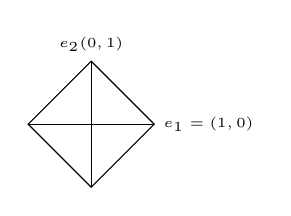
\begin{tikzpicture}[scale=.4]
	    \draw (-.5,0) -- (1.5,2) -- (3.5,0) -- (1.5,-2) -- cycle; % Dibuja el rombo
	    \draw (-.5,0) -- (3.5,0)node[right]{\tiny$e_1=(1,0)$}; % Dibuja la línea horizontal
	    \draw (1.5,2)node[above]{\tiny$e_2(0,1)$} -- (1.5,-2); % Dibuja la línea vertical
	\end{tikzpicture}
    \end{center}
    Donde, $e_1$ y $e_2$ se llaman extremales.

\begin{center}
    \begin{tikzpicture}[scale=0.8,>=Triangle]
      \draw(-2.5,-1.5) -- (1.8,-1.5) -- (2.8,-.7);
      \draw(3.2,-1.5)node[above]{\small$B(0,1)$};
      \draw[dashed](2.8,-.7) -- (-1.5,-.7);
      \draw(-1.5,-.7) -- (-2.5,-1.5);
	\draw[<-] (-1.5,0) -- (0,-2);
	\draw[<-] (1.5,0) -- (0,-2);
	\draw[<-] (-.3,-.5) -- (0,-2);
	\draw[<-,dashed] (.5,.4) -- (0,-2);
	\draw[opacity=.5](-1.5,0) -- (.5,.4) -- (1.5,0) -- (-.3,-.5) -- cycle;
	\draw[opacity=.5](-.75,-1) -- (0.25,-.8) -- (.75,-1) -- (-.15,-1.3) -- cycle;
	\draw[opacity=.3] (-1.5,-2) -- (1.5,-2); % recta horizontal
	\draw[opacity=.3] (-.7,-2.5) -- (.6,-1.6); % recta vertical
    \end{tikzpicture}
\end{center}
    \item $\|\cdot\|_\infty: \mathbb{R}^n\to \mathbb{R}$, $\|x,y\|_\infty=\max\left\{|x|,|y|\right\}$. Compara y coge la más grande. Veamos una vista transversal con respecto del cono:
    \begin{center}
	\begin{tikzpicture}[scale=.7]
	    \draw (-2,0) -- (2,0);
	    \draw (0,-2) -- (0,2);
	    \draw[dashed] (1,-2) -- (1,2);
	    \draw[dashed] (-1,-2) -- (-1,2);
	    \draw[dashed] (-2,1) -- (2,1);
	    \draw[dashed] (-2,-1) -- (2,-1);
	    \pattern[pattern=north east lines, pattern color=gray!35, rotate around={0:(1,6)}] (-1,-1) rectangle (1cm,1cm);
	\end{tikzpicture}
    \end{center}

    \item $\|\cdot\|_P: \mathbb{R}^n\to \mathbb{R}$, $p\in (1,\infty).$ (Existe una especie de promedio)

    \switchcolumn[1]*{\noindent\scriptsize
    \begin{itemize}
	\item La norma infinito es cómo la madre de todas las demás normas. Representamos con un cuadrado sobre la base canónica.
	\item La norma 1 sera el rombo que ya dibujamos.
	\item La Euclídea será un círculo.
	\item Cuando $p<1$ no será una función convexa. (No se cumplirá la desigualdad triangular). Ya no será una bola.
    \end{itemize}
}
    \switchcolumn[0]\noindent
	$$\|(x,y)\|=\sqrt[p]{|x|^p+|y|^p}$$
	En particular: 
	$$\|(x,y)\|_2=\sqrt{|x|^2+|y|^2}.$$
    \begin{center}
	\begin{tikzpicture}[scale=.7,>=Triangle]
	    \draw (-2,0)node[left]{\tiny$-e_1$} -- (2,0)node[right]{\tiny$e^1$};
	    \draw (0,-2)node[below]{\tiny$e_2$} -- (0,2)node[above]{\tiny$-e_2$};
	    \draw (2,-2) -- (2,2);
	    \draw (-2,-2) -- (-2,2);
	    \draw (-2,2) -- (2,2);
	    \draw (-2,-2) -- (2,-2);
	    \draw[blue] (-2,0) -- (0,2) -- (2,0) -- (0,-2) -- cycle;
	    \draw[red] (0,0) circle (2cm);

	    \draw[<-,brown](1.7,1.7)--(2.2,1.7)node[right]{$p\in(2,\infty)$};
	    \draw[<-,green](1.3,1.2)--(2.2,1.2)node[right]{$p\in(1,\infty)$};
	    \draw[gray](1,0)node[above left]{\tiny$p<1$};

	    %semilunas entre los ejes
	    \draw[green](0,2)..controls(1.3,1.3)..(2,0)..controls(1.3,-1.3)..(0,-2)..controls(-1.3,-1.3)..(-2,0)..controls(-1.3,1.3)..(0,2);
	    \draw[brown](0,2)..controls(1.8,1.8)..(2,0)..controls(1.8,-1.8)..(0,-2)..controls(-1.8,-1.8)..(-2,0)..controls(-1.8,1.8)..(0,2);
	    \draw[gray](0,2)..controls(.5,.5)..(2,0)..controls(.5,-.5)..(0,-2)..controls(-.5,-.5)..(-2,0)..controls(-.5,.5)..(0,2);
	\end{tikzpicture}
    \end{center}
\end{enumerate}


\section{Poliedros}

\switchcolumn[1]*{\noindent\scriptsize
    \begin{itemize}
	\item La idea de los semiespacios afines, de tomar un hiperplano de un lado y el otro, en realidad se puede hacer con hiperplanos o cualquier subespacio afín.
	\item Un polihedro será prácticamente una cantidad finita de caras. Es decir, son hiperespacio de dimensión $n-1$ que determinan la frontera, tomando desigualdades $a_j^Tx\leq b_j$. El cual es un semiespacio determinado por la dirección del hiperplano $a_j$. Y el $b_j$ es una traslación.
	\item Cuando se pide varias condiciones es la intersección de semiespacios.
	\item $c_j^Tx=d_j$, me fija hiperplanos, que justo corte por un lugar específico.
	\item Los poliedros son aplicados a optimización lineal.
    \end{itemize}
}
\switchcolumn[0]\noindent
$$P=\left\{x\in \mathbb{R}^n : a_j^T x \leq b_j, j=1,\ldots,n,  c_j^T x \leq d_j, k=1,\ldots,p \right\}.$$

\begin{center}
    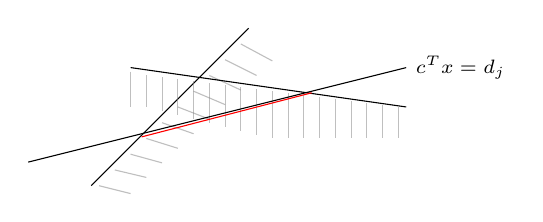
\begin{tikzpicture}[scale=1]
	\draw(0,0) -- (2,2);
	\draw[gray,opacity=.5](.1,0) -- (.5,-.1);
	\draw[gray,opacity=.5](.3,.2) -- (.7,.105);
	\draw[gray,opacity=.5](.5,.4) -- (.9,.29);
	\draw[gray,opacity=.5](.7,.6) -- (1.1,.475);
	\draw[gray,opacity=.5](.9,.8) -- (1.3,.66);
	\draw[gray,opacity=.5](1.1,1) -- (1.5,.845);
	\draw[gray,opacity=.5](1.3,1.2) -- (1.7,1.03);
	\draw[gray,opacity=.5](1.5,1.4) -- (1.9,1.215);
	\draw[gray,opacity=.5](1.7,1.6) -- (2.1,1.4);
	\draw[gray,opacity=.5](1.9,1.8) -- (2.3,1.585);

	\draw(.5,1.5) -- (4,1);
	\draw[gray,opacity=.5](.5,1.45) -- (.5,1);
	\draw[gray,opacity=.5](.7,1.4) -- (.7,1);
	\draw[gray,opacity=.5](.9,1.375) -- (.9,.95);
	\draw[gray,opacity=.5](1.1,1.35) -- (1.1,.9);
	\draw[gray,opacity=.5](1.3,1.325) -- (1.3,.85);
	\draw[gray,opacity=.5](1.5,1.3) -- (1.5,.8);
	\draw[gray,opacity=.5](1.7,1.275) -- (1.7,.75);
	\draw[gray,opacity=.5](1.9,1.25) -- (1.9,.7);
	\draw[gray,opacity=.5](2.1,1.225) -- (2.1,.65);
	\draw[gray,opacity=.5](2.3,1.2) -- (2.3,.6);
	\draw[gray,opacity=.5](2.5,1.175) -- (2.5,.6);
	\draw[gray,opacity=.5](2.7,1.15) -- (2.7,.6);
	\draw[gray,opacity=.5](2.9,1.125) -- (2.9,.6);
	\draw[gray,opacity=.5](3.1,1.1) -- (3.1,.6);
	\draw[gray,opacity=.5](3.3,1.075) -- (3.3,.6);
	\draw[gray,opacity=.5](3.5,1.05) -- (3.5,.6);
	\draw[gray,opacity=.5](3.7,1.025) -- (3.7,.6);
	\draw[gray,opacity=.5](3.9,1) -- (3.9,.6);

    \draw(-.8,.3) -- (4,1.5)node[right]{$c^Tx = d_j$};
    \draw[red] (.64,.62) -- (2.8,1.18);
    \end{tikzpicture}
\end{center}

El poliedro generaliza:

\begin{itemize}
    \item Linea, 
    \item segmento, 
    \item semiespacio, 
    \item subespacio afín.
\end{itemize}

Sin embargo no todo conjunto convexo se puede definir cómo un poliedro.


\section{Operaciones que conservan la convexidad}

Algunas propiedades que conservan la convexidad:

    \switchcolumn[1]*{\noindent\scriptsize
	\begin{itemize}
	    \item Las aplicaciones afines cuando trabajamos en $\mathbb{R}^n$ y $\mathbb{R}^m$ son tan sencillas como multiplicar una matriz y sumar un número. Es una aplicación lineal y sumar una constante, es decir trasladar.
	    \item El hecho que funcione para adelante y para atrás, nos permite que para que una función sea convexa yo puedo demostrar que su imagen de $f$ es convexa. Donde se nos simplifica las cosas.
	    \item Si un convexo esta lejos del cero, dado que la traslación es afín, podemos trasladar a cero demostrarlo y llevarlo a su estado original. Así sin perdida de generalidad podemos asumir que el cero está en el conjunto.
	\end{itemize}
}
\switchcolumn[0]\noindent
\begin{enumerate}[\bfseries 1.]
    \item Intersección de convexos es convexo.
    \item Si tenemos una función $f:\mathbb{R}^n\to \mathbb{R}^m$, $f$ afín. Es decir, 
    $$\left(f(x)=Ax+b, A\in \mathcal{M}_{m\times n} \text{ y } b\in \mathbb{R}^m\right).$$
\item Si tengo un conjunto $C\subseteq \mathbb{R}^n$ convexo. Entonces, $f(c)$ es convexo. Si $B\subseteq \mathbb{R}^n$ convexo, entonces ($f^{A}(B)$) la anti-imagen de $B$ es también convexo. 
\end{enumerate}

Algunos ejemplos particulares de afín:
\switchcolumn[1]*{\noindent\scriptsize
    \begin{itemize}
	\item Si 2., entonces se cumple 3. Lo que se puede ver es que los primeros tres ejemplos son estables, la imagen por una homotecia o la anti-imagen, etc.
	\item La suma de dos cosas convexas es convexa.
	\item El producto cartesiano de dos cosas convexas es convexa.
	\item Estas dos últimas son un poco más difíciles de demostrar porque hay que pensar que funciones afines nos da la suma de Minskowsky y que función afín nos da el producto de dos conjuntos. En realidad, se utiliza la pre-imagen.
    \end{itemize}
}
\switchcolumn[0]\noindent
\begin{itemize}
    \item  Homotecias: Multiplicar por un escalar.
    \item Translaciones.
    \item Proyecciones: Aplicaciones lineales importantes.
    \item Suma de Minskowsky.
	Empezamos con dos conjuntos y definimos la suma de Minkowski como el conjunto de los $A$, $B$ tal que la $A$ está en $A$ y la $A$ en $B$, lo podemos ver como la imagen aplicación afín de un conjunto convexo.
    \item Producto de dos conjuntos.
\end{itemize}


\section{Desigualdad generalizadas}

¿Cual de los dos puntos es más importante?. Es los puntos donde están pintados, dependiendo si es máximo o mínimo.

\begin{center}
    \begin{tikzpicture}[scale=.7]
	\draw[] (-.5,0) -- (4,0);
	\draw[] (0,-.5) -- (0,4);
	%Dibujar dos puntos en el primer cuadrante
	\draw[fill=black] (1.5,1.5) circle (2pt);
	\draw[fill=black] (3,3) circle (2pt);
	\pattern[pattern=north east lines, pattern color=gray!35, rotate around={0:(0,0)}] (4,4) rectangle (1.4cm,1.35cm);
	\draw[fill=black] (.8,2.5) circle (2pt);
	\pattern[pattern=north east lines, pattern color=blue!20, rotate around={0:(0,0)}] (4,4) rectangle (.7,2.35);
    \end{tikzpicture}
\end{center}

Ahora, cual es mejor de estos dos conjuntos.

Esto se define como:
$$
\begin{array}{rcl}
    x,y\in \mathbb{R}^n, x\leq y &\Leftrightarrow& x_i\leq y_i, \quad i=1,\ldots,n\\\\
				 &\Leftrightarrow& 0\leq y_i-x_i, \quad i=1,\ldots,n\\\\
				 &\Leftrightarrow& y-x\in \mathbb{R}^n_+\\\\
				 &\Leftrightarrow& y\in x+\mathbb{R}^n_+. \quad (\text{Minkowski})
\end{array}
$$

Ahora, en vez de utilizar $\mathbb{R}^n_+$ puede utilizarse otro conjunto $K$. Ahora, ¿Qué propiedades debería tener $K$, para tener un conjunto con orden?. Necesito asignar  una serie de propiedades que tiene $\mathbb{R}^n$.

Por lo que definimos de cono propios

% ------------------- DEFINICION
\begin{def.}\,\\
    $K\subseteq \mathbb{R}^n$ es cono propio si es un cono:
    \begin{enumerate}[i)]
	\item Convexo: Cualquier parte de puntos el segmento estará en el mismo conjunto. Buen comportamientos de las SUMAS.
	\item Cerrado: Vamos a definir con el menor o igual.
	\item Sólido ($\interior(K)\neq \emptyset$): Que pueda decidir en todo $\mathbb{R}^n$. Para ello, debo tener al menos un punto interior.
	\item Apuntado ($x\in K,  -x\in K\Rightarrow x=0$): No me deja que contenga una recta entera.
    \end{enumerate}
\end{def.}

\switchcolumn[1]*{\noindent\scriptsize
    \begin{itemize}
	\item Está claro que es convexo.
	\item Ya que no se tiene dos $++$, en $\mathbb{R}^n_+$. Entonces es cerrado.
	\item Sólido, ya que existe cualquier punto interior. Los bordes no son puntos interiores.
	\item Apuntado, ya que, cuando tengo un punto tiene opuesto. Básicamente tiene que pasar siempre en cero.
    \end{itemize}
}
\switchcolumn[0]\noindent
\begin{center}
    \begin{tikzpicture}[scale=.5]
	\draw[] (-2,0) -- (4,0);
	\draw[] (0,-2) -- (0,4);
	\pattern[pattern=north east lines, pattern color=blue!20, rotate around={0:(0,0)}] (0,0) rectangle (4,4);
	\draw[](4,4)node[]{$\mathbb{R}^n_+$};
	\draw[](-4,-4)node[]{$\mathbb{R}^n_-$};
	\pattern[pattern=north east lines, pattern color=black!20, rotate around={0:(0,0)}] (0,0) rectangle (-4,-4);
    \end{tikzpicture}
\end{center}


\switchcolumn[1]*{\noindent\scriptsize
    \begin{itemize}
	\item Cada $K$ que fijemos será una lección de multicriterio.
	\item Si estoy en $\mathbb{R}^n$ por ejemplo, entonces tengo cinco conos para elegir, y según un criterio de esas 5 variables definiremos cual es mejor o cual es peor. 
	\item Estos criterios lo puedo definir mediante conos.
	\item Me asegura un sistema sistemático de orden.
    \end{itemize}
}
\switchcolumn[0]\noindent
Dado un cono propio $K\subseteq \mathbb{R}^n$ se define $\leq_K$ un orden en $\mathbb{R}^n$ como:
$$
\begin{array}{rlc}
    x\leq_K y &\Leftrightarrow& y-x\in K\\\\
	      &\Leftrightarrow& y\in x+K.
\end{array}
$$

Ejemplo: Si tomamos  dos puntos. Entonces,
\begin{center}
    \begin{tikzpicture}
	\draw(-1,0) -- (2,0);
	\draw(0,-1) -- (0,2);
	\draw[pattern=north east lines,pattern color=gray!30, rotate around={-45:(0,0)}] (-.7,2) -- (0,0) -- (.7,2);
	\draw(-1,0) -- (2,0);
	\draw(0,-1) -- (0,2);
	\draw[pattern=north east lines,pattern color=gray!30, rotate around={-45:(3.5,-5)}] (-.7,2) -- (0,0) -- (.7,2);
	\draw(3.5,0) -- (6.5,0);
	\draw(4,-1) -- (4,2);

	%dibujar dos puntos
	\draw[fill=black] (4.55,1.02) circle (1.5pt);
	\draw[fill=black] (6,.8) circle (1.5pt);

    \end{tikzpicture}
\end{center}

Aquí no puedo asegurar que $x\not\leq_K y.$

% -------------------- EJERCICIO 2.5
{\color{blue}
\begin{ejer}
    Demuestra que $\leq_K$ es un orden.
    \begin{enumerate}[i)]
	\item Reflexiva, $x\leq_K x \; \forall x.$
	\item Transitiva, $x\leq_K y, y\leq_K z \Rightarrow x \leq_K z$.
	\item Antisimétrica, $x\leq_Ky, t\leq_k x \Rightarrow x=y$..
	\item Estable para sumas: $x\leq_K y, z\leq_K w \Rightarrow y\pm w$.
	\item Estable para productos positivos: $x\leq_K y \Rightarrow \lambda x\leq_K \lambda y, \lambda >0$.
	\item Estable para límites: $x_n\leq_K y, x_n\to x \Rightarrow x\leq_K y$.
    \end{enumerate}
	    Demostración.-\; Para demostrar debemos utilizar las propiedades de cono propio. Lo que le pido que al orden se comporte bien con las sumas, con los productos por escalares positivos y que se comporte bien con los límites por lo que pido que el cono sea cerrado.
\end{ejer}
}

\section{Teorema de separación y extensión}
\switchcolumn[1]*{\noindent\scriptsize
\begin{center}
    \begin{tikzpicture}[rotate=45, >=Triangle,scale=.5]
	\draw (0,0) ellipse (2cm and 1cm);
	\draw(-1,2)node[right]{$A$};
	\draw[red](-1,-3)--(3,0);
	\fill(2.2,-1.2)node[right]{$x_0$}circle(2pt);
    \end{tikzpicture}
\end{center}

    \begin{center}
      \begin{tikzpicture}[rotate=45,scale=0.6]
	\coordinate (A) at (-2,0);
	\coordinate (B) at (6,0);
	\coordinate (C) at (11,3);
	\coordinate (D) at (3,3);
	\coordinate (Center) at ($(A)!0.5!(C)$);
	\draw[] ($(Center)+(-1,.5)$) .. controls ($(Center)+(0.2,2)$) and ($(Center)+(3,-.1)$) .. ($(Center)+(1,-.4)$) .. controls ($(Center)+(0,-.5)$) and ($(Center)+(-1,.5)$) .. ($(Center)+(-.8,-.9)$) .. controls ($(Center)+(-.5,-2)$) and ($(Center)+(-3.5,-.5)$) .. ($(Center)+(-1,.5)$);
	\draw[red](6,3)--(3,0);
	\fill(4.2,1)node[right]{$x_0$}circle(2pt);
	\draw(3.5,3.5)node[right]{$A$};
      \end{tikzpicture}
    \end{center}
}
\switchcolumn[0]\noindent
\begin{tcolorbox}[colframe=white]
    \begin{itemize}
	\item La idea fundamental es que un conjunto convexo siempre se puede aproximar por tangentes.
	\item Los hiperplanos nos ayudaran a cortar el espacio, donde a un lado nos dejaran al conjunto y al otro nada.
	\item Moviendo esos hiperplanos, alrededor del conjunto podemos recuperar toda la forma del conjunto.
	\item Esto nos dan pie a unos teoremas que nos dice que si tenemos un conjunto y un punto que está fuera, yo siempre puedo encontrar una linea recta que los separa.
	\item Si el conjunto no es convexo y el punto a separar está en la región "no convexa". Entonces, no podemos separarlas con hiperplanos o semiespacios.
    \end{itemize}
\end{tcolorbox}

\switchcolumn[1]*{\noindent\scriptsize
\begin{itemize}
    \item Este lema nos encuentra elementos maximales. 
    \item Maximal significa que no tiene un elemento por encima, si hay otro, entonces es el mismo.
    \item Sea un conjunto $\mathscr{A}$ parcialmente ordenado, con elementos en fila dentro un conjunto $\mathscr{C}$. Si $\mathscr{A}$ toma la forma de $\mathscr{C}$, siempre estará acotado superiormente. 
\end{itemize}
}
\switchcolumn[0]\noindent
%-------------------- Lema 2.1
\begin{lema}[Lema de Zorn] Si tengo un conjunto $\left(\mathscr{A},\leq\right)$ parcialmente ordenado, tal que si $\mathscr{C} \subseteq \mathscr{A}$ totalmente ordenado $\left(x,y \in \mathscr{C} \Rightarrow x\leq y \text{ ó } y\leq x\right)$, tiene una cota superior en $\mathscr{A}$ $\left(\exists a\in \mathscr{A}:x\leq a \;\forall x\in \mathscr{C}\right)$. Entonces, $\mathscr{A}$ tiene un maximal ($\exists a \in \mathscr{A}: b \in \mathscr{A},\; b\leq a \Rightarrow b=a$). $\left[\mathscr{A}\notin \emptyset\right]$.
\end{lema}


\switchcolumn[1]*{\noindent\scriptsize
    \begin{itemize}
	\item Este lema es el mismo enunciado del teorema de abajo, pero no para cualquier subespacio sino para un espacio de co-dimensión. Yo se demostrar que si tengo una función en un hiperplano yo puedo extenderla a una dimensión. 
	\item Con este lema 2.2 podemos realizar operaciones finitas sin necesitad de lema de Zorn.
	\item Si tenemos un espacio y tenemos un hiperplano y en el hiperplano tenemos las condiciones del teorema. Entonces somos capaces de encontrar una extensión a todo el espacio que sigue siendo lineal que extiende a la $g$ y además está controlada por $p$.
    \end{itemize}
}
\switchcolumn[0]\noindent

%-------------------- Lema 2.2
\begin{lema}
    Si un espacio vectorial $H+[x_c]$ y unas funciones $g:H\to \mathbb{R}$ lineal y $p:H+[x_c]\to \mathbb{R}$ lineal. Cumple que $g(h)\leq p(h)\; \forall h\in H$. Entonces, $\exists\; \overline{g}:H+[x_0]\to \mathbb{R}$ lineal, tal que $\overline{g}(h)=g(h)$ y $\overline{g}(x)=g(x)\; \forall x\in H+[x_0]$.

	Demostración.-\; Dado $g:H\to \mathbb{R}$ lineal, tal que $g(h)\leq p(h)\; \forall h\in H$. Quiero definir $\overline{g}:H+[x_0]\to \mathbb{R}$ lineal y que $g(x)\leq p(x)\; \forall x\in H+[x_0]$. Dado que $[x_0]$ es linealmente independiente a $g(h)$, por lo tanto
	$$\overline{g}\left(h+\lambda x_0\right)=\overline{g}(h)+\lambda \overline{g}(x_0)=\alpha=g(h)+\lambda \alpha.$$
	Ahora, debemos definir $[x_0]$ para que funcione la cosa. Para ello buscamos $\alpha\in \mathbb{R}$ tal que $g(h)+\lambda x_0\leq p(h)+\lambda x_0\; \forall h\in H, \;\forall \lambda\in \mathbb{R}.$
	Esto será equivalente A:
	$$
	\left\{
	    \begin{array}{rcl}
		g(x)+\alpha&\leq&p(h+x_0),\; \forall h\in H\\
		g(h)-\alpha&\leq&p(h-x_0),\; \forall h\in H
	    \end{array}
	\right. \qquad (1)
	$$
	$$\Updownarrow$$
	$$g(x)-p(x-x_0)\leq \alpha \leq p(y-x_0)-g(y)\; \forall x,y\in H.$$
	Se puede poner $x,y$ en vez $h$ ya que las desigualdades de $(1)$ son independientes.

	Ya que queremos encontrar un número $\alpha$ que cumpla esta última desigualdad. Intentaremos probar que el supremo de lo que tenemos a la izquierda es menor o igual de las cosas que tenemos a derecha. Es decir,
	$$\sup\left\{g(x)-p(x-x_0)\right\},x\in H\leq \inf\left\{p(y-x_0)-g(y)\right\},y\in H.$$
	$$\Updownarrow$$
	$$g(x)-p(x-x_0)\leq p(y+x_0)-g(y)\; \forall x,y\in H.$$
	(Muchas veces para demostrar tomamos algo que no sabemos que es cierta y con equivalencias llegamos a algo que si sabemos que es cierta). Entonces, 
	$$g(x)+g(y)\leq p(x-x_0)+p(y+x_0)$$
	$$\Updownarrow$$
	$$g(x+y)\leq p(x-x_0)+p(y+x_0)$$
	Dado que $g(x+y)$ está controlada por la $p$, se tiene
	$$g(x+y)\leq p(x+y)$$
	Cómo $p$ está definida en todo el espacio y es sublineal, obtenemos
	$$
	\begin{array}{rcl}
	    g(x+y)&\leq& p(x+y)\\\\
		  &=& p(x-x_0+y+x_0)\\\\
		  &\leq& p(x-x_0)+p(y+x_0).
	\end{array}
	$$
	Esta última desigualdad es cierta, por lo que queda demostrada el lema.
\end{lema}

\begin{itemize}
    \item Extender funciones lineales es sumamente sencillo: Por ejemplo si estamos en $\mathbb{R}^3$ y tenemos una función lineal definida en el plano, lo único que tenemos que hacer es tomar una base del plano, completarla a la base del espacio y en ente caso como es $\mathbb{R}^3$ y $\mathbb{R}^2$, sería solamente un vector. Entonces, definimos una aplicación lineal que coincida con $g$ en el plano y en el vector que sobra le damos el valor cero.
\end{itemize}

\switchcolumn[1]*{\noindent\scriptsize
\begin{itemize}
    \item La idea es extender combinaciones lineales.
    \item Es \textbf{sublineal} si $p(x+y)\leq p(x)+p(y)$ y $p(\lambda x)=\lambda p(x)$ si $\lambda>0$.
    \item La función $g$ lineal es controlada por esa función norma $p$. Quiere decir que es continua en la métrica $g$ de $p$. 
    \item La idea es la siguiente: tengo un subespacio, una función lineal definida en el subespacio y que está contralada por $p$.
    \item Yo tengo una distancia en todo mi espacio, una aplicación lineal definida abajo y puedo extenderla.
\end{itemize}
}

\switchcolumn[0]\noindent
% -------------------- TEOREMA  2.3
\begin{teo}[Teorema de Hahn-Banach (Extensión)]\,
    Sea $E$ un espacio vectorial y una función $p:E\to \mathbb{R}^+$ sublineal. Sea también $E_0\subseteq E$, $g:E_0\to \mathbb{R}$ lineal y $g(x)\leq p(x)\,\forall x\in E_0$. Entonces existe $\overline{g}:E\to \mathbb{R}$ lineal, tal que $\overline{g}(x)=g(x)\,\forall x\in E_0$ ($\overline{g}$ extiende a $g$) y $\overline{g}(x)\leq p(x),\, \forall x\in E$.

	Demostración.-\; Si yo quiero comenzar por una función $g$, en un espacio pequeño y quiero extenderlo a un espacio grande, debo comenzar por tomar todas las distribuciones.

	Empezamos definiendo de objetos, en este caso extensiones como,
	$$f=\left\{(E_1,g_1):
	    \begin{array}{l}
		g_1:E_1\to \mathbb{R} \text{ lineal}\\
		g_1(x)=g(x)\; \forall x\in E_0\\
		E_0\subseteq E_1\\
		g_1(x)\leq p(x)\; \forall x\in E_1.
	    \end{array}
	\right\}$$
\switchcolumn[1]*{\noindent\scriptsize
    \begin{itemize}
	\item $f$ es no vacío porque la función inicial $g$ y el subespacio $E_0$ están ahí.
	\item La idea de este teorema se basa en que tengo una $g$ que la extiendo por muchas ramas, donde cada extensión las puedo extender de nuevo por más ramas. Pero cuando tomo la cadena totalmente ordenado solo me estaré yendo por una rama. Donde las $g$ van coincidiendo a través de las ramas. Básicamente la $f$ es un árbol y la $g$ es una rama bien ordenada.
    \end{itemize}
}
\switchcolumn[0]\noindent
	Lo primero que justifico es el vacío. Es decir, 
	$$f \notin \emptyset,\text{ ya que } (E_0,g)\in f.$$
	Ahora, introducimos un orden en esta familia, de forma que una de estas extensiones sea mejor que otra. Dos los dos elementos definidos, 
	$$(E_1,g_1)\leq (E_2,g_2).$$
	Al definir esto, no decimos que todos los elementos se puedan comparar. Lo que decimos es que si yo tomo estos elementos se cumplirán siempre que se cumpla las siguientes condiciones:
	\begin{itemize}
	    \item $E_1\subseteq E_2$.
	    \item $g_1(x)=g_2(x)\; \forall x\in E_1.$
	\end{itemize}
	El conjunto 
	$$\left(f,\leq\right)$$
	se llama parcialmente ordenado.

	Ahora demostraremos que que este conjunto parcialmente ordenado, toda cadena $\mathscr{C}\subseteq \mathscr{A}$ tiene una cota superior, y por el lema de Zorm tiene un elemento maximal.

	Si $\mathscr{C}\subseteq f$ es una cadena totalmente ordenado. Lo que queremos encontrar un elemento no necesariamente en $\mathscr{C}$ pero si en $f$ que sea una cota superior. Para ello,
	$$\mathscr{C}=\left\{\left(E_i,g_i\right)\right\}_{i\in I}$$
	Ahora, definimos 
	$$E_{\mathscr{C}}=\bigcup_{i\in I} E_i.$$
	Dados dos que yo fije, uno mayor que otro, siempre tendré inclusión. Por eso nos sirve la unión. Porque están contenido uno debajo del otro.

	Definimos también 
	$$g_{\mathscr{C}}:E_{\mathscr{C}}\to \mathbb{R}.$$
	Lo que tendrá que coincidir con las $g_i$. Por lo que,
	$$g_{\mathscr{C}}(x)=g_i(x)\; \text{ si } x\in E_i.$$
	Dado que $g_i$ cumplen  $g_1(x)\leq p(x)\; \forall x\in E_1$. Entonces, en lo particular 
	$$g_{\mathscr{C}}(x)\leq p(x)\; \forall x\in E_{\mathscr{C}}.$$
	Así,
	$$\left(E_{\mathscr{C},g_{\mathscr{C}}}\right)\in f.$$
	Y además,
	$$\left(E_{\mathscr{C}},g_{\mathscr{C}}\right)\geq \left(E_i,g_i\right)\; \forall i\in I.$$
\switchcolumn[1]*{\noindent\scriptsize
	¿Qué haremos con ese elemento maximal?. Lo ideal es que $\overline{E}$ sea todo el $E$, pero podría ser que no. ¿Qué pasa si $\overline{E}$ se encuentra por debajo de $E$?. En otras palabras, no llegue a extender a todo el espacio vectorial.
}
\switchcolumn[0]
	Donde $\left(E_{\mathscr{C},g_{\mathscr{C}}}\right)$ es una cota superior de $\mathscr{C}.$

	Por lo tanto, por el lema de Zorm existe $\left(\overline{E},\overline{g}\right)\in f$ que es un elemento maximal de $f$.
\switchcolumn[1]*{\noindent\scriptsize
    Cuando tomamos $[x_0]$ quiere decir que tomo la linea generada por $x_0$ (span).
} 
\switchcolumn[0]
	Ahora, demostraremos que $\overline{E}$ es efectivamente la $E$. Para ello, utilizaremos una reducción al absurdo. Supongamos que $\overline{E}\subsetneq E$. Entonces existe un $x_0\in \overline{E} \backslash E$. Por lo que puedo ampliar $\overline{E}$ de la siguiente forma:
	$$\overline{E} \subsetneq \overline{E}+[x_0]\subseteq E.$$
	Lo que intentaremos probar por contradicción es que si $\overline{E}$ no fuese $E$. $\overline{E}$ no puede ser un elemento maximal. Por el lema 2.2, aplicado a $H=\overline{E}$ y a $\overline{g}:E\to \mathbb{R}$. Existe una extensión $\overline{g}:E+[x_0]\to \mathbb{R}$ tal que 
	$$\overline{g}(x)\leq p(x)\; \forall x\in \mathbb{E}+[x_0].$$
	Ahora, $$\left(\overline{E}+[x_0],\overline{g}\right)\in f\lneq \overline{E},\overline{g}.$$ 
	Por lo que es imposible pues $\left(\overline{E},\overline{g}\right)$ es un elemento maximal. Luego, $\overline{E}=E$  y $\left(\overline{E},\overline{g}\right)$ es la extensión buscada.
\end{teo}

\begin{tcolorbox}[colframe=white]
    Ahora el objetivo es establecer los resultados de separación y ver la conexión con el teorema de extensión. 
\end{tcolorbox}

En principio será importante ver un punto interior y separar un punto del conjunto. Tal como lo veremos a continuación:

\begin{center}
    \begin{tikzpicture}[rotate=45, >=Triangle,scale=.7]
	\draw (0,0) ellipse (2cm and 1cm);
	\draw(-1,2)node[right]{$A$};
	\draw[blue](-2.4,.95)--(3.2,-1.65);
	\fill(2.2,-1.2)node[below right]{$x_0$}circle(2pt);
	\fill(-.4,0)node[below right]{$0$}circle(2pt);
	\fill(1.7,-.98)node[below right]{}circle(2pt);
	\draw[red,dashed](1.7,2.95)--(1.7,-3.65)node[below]{$p$};
	\draw[red](-1,-3)--(3,0)node[above]{$p$};
    \end{tikzpicture}
\end{center}

Nos olvidamos del plano y nos fijamos en la linea. Esta linea es una aplicación lineal. Y por el teorema de Hahn-Banach extiendo. Pero debemos aseguramos que la extensión no se meta en el conjunto, que es precisamente de lo que se encarga $p$. Esta $p$ a escoger dependerá del conjunto $A$ y la elección de $p$ me permitirá, que cuando yo tome la extensión se extienda fuera de $A$. Ahora, ¿cuál es la $p$ que se definirá a partir del conjunto $A$?. Esta $p$ se llama funcional me Minskowsky, y nos hará falta definir el concepto de interior. En dimensión infinita el concepto que mencionaremos a continuación es diferente y en $\mathbb{R}^n$ son lo mismo.


%-------------------- DEFINICIÓN 2.15
\begin{def.}
    Si $S\subseteq E$,
    \begin{enumerate}[1)]
	\item $x_0\in S$ es un punto interior algebraico. Es decir, si $\forall x\in E$, existe un $\epsilon>0$ tal que $\left]x_0-\epsilon,x_0+\epsilon\right[\subseteq S$. (Quiere decir que dependiendo de la dirección existirá un $\epsilon$).
	\begin{center}
	    \begin{tikzpicture}[rotate=45, >=Triangle,scale=.7]
		\draw[opacity=.7] (0,0) ellipse (2cm and 1cm);
		\draw(-1,2)node[right]{$A$};
		\draw[blue](-2.4,.95)--(3.2,-1.65);
		\fill(-.4,0)node[below]{\tiny$0$}circle(2pt);
		\node[above, red] at (1,-.5) {\tiny$x_0+\epsilon$};
		\node[above, red] at (.3,-.2) {\tiny$x_0-\epsilon$};
		\draw[red] (1,-.6) node {$[$};
		\draw[red] (.3,-.3) node {$]$};
	    \end{tikzpicture}
	\end{center}

	\item $S^i=  \left\{x\in S: x\text{ es interior algebraico a } S\right\}$.
	\item $x_0$ es un punto de clausura algebraica de $S$, si existe $x\in E$ tal que el intervalo $\left[x,x_0\right)\in S$.
	\begin{center}
	    \begin{tikzpicture}[rotate=45, >=Triangle,scale=.7]
		\draw[opacity=.7] (0,0) ellipse (2cm and 1cm);
		\draw(-1,2)node[right]{$A$};
		\draw[blue](1.4,-.7)--(.27,-.3);
		\fill(-.4,0)node[above left]{\tiny$0$}circle(2pt);
		\node[above, red] at (1.35,-.5) {\tiny$x$};
		\node[above, red] at (.3,-.15) {\tiny$x_0$};
		\draw[red] (1.4,-.7) node {$)$};
		\draw[red] (.3,-.3) node {$[$};
	    \end{tikzpicture}
	\end{center}
	\item $S^c$ son los puntos de clausura algebraica de $S$.
	    $$S^i = \interior(S)\in \mathbb{R}^n$$
	    $$S^c = \text{ al cierra de } S \text{ en } \mathbb{R}^n \text{ si } S \text{ es convexo.}$$
    \end{enumerate}
\end{def.}

Lo que necesitamos es definir un punto interior

\switchcolumn[1]*{\noindent\scriptsize
    \begin{itemize}
	\item $0\in S^i$ significa que el cero pertenece al interior algebraico de $S$.
	\item La idea de esta definición, es que en vez de tomar la recta, tomaremos una semirecta, que empieza en el cero y se va a más infinito. Cómo el elipsoide es convexo, los bordes serán mi forma de medir (será la $p$ del teorema 2.3), donde hasta el margen valdrá $1$, la mitad $1/2$ y el doble $2$.
	\item Debemos hacer que se cumple 1) de la definición 2.15. Es decir, que exista un valor $\epsilon$ que se quede dentro del conjunto.
	\item Básicamente lo que nos dice el funcional de Minkowski que está dentro o fuera de un conjunto.
    \end{itemize}
}
\switchcolumn[0]
%-------------------- DEFINICIÓN 2.16
\begin{def.}
    Sea $S\subseteq E$, $0\in S^i$. Se define el funcional de Minkowski asociado a $S$ cómo:
    $$P_S(x) = \inf\left\{\lambda>0: x\in \lambda S\right\}.$$
\end{def.}

%-------------------- PROPIEDAD 2.3
\begin{prop}
    $S$ convexo, $0\in S^i$.
    \begin{enumerate}[1)]
	\item $S^i=\left\{x\in E: p(x) < 1 \right\}\subseteq S \subseteq \left\{x\in E:p_S(x)\leq 1\right\}=S^c$.
	\item $p_S=p_{S^i}=p_{S^c}$
	\item $p_S\geq 0$ es sublineal, sii los puntos de $p$ son menores iguales a $1$. Y si consigo que sean mayores que uno, las cosas están fuera. En otras palabras, nos permite decidir si estoy fuera o estoy dentro.
	\switchcolumn[1]*{\noindent\scriptsize
	    \begin{itemize}
		\item Los funcionales lineales no negativos están en correspondencia univoca con los conjuntos. Es decir, dame un sublineal encuentro un conjunto y viceversa.) 
		\item Si estamos trabajando con normas, dame una norma y te doy una bola unidad. La bola unidad es el conjunto que define la norma y la norma se define a partir de la bola unidad.
	    \end{itemize}
	}
	\switchcolumn[0]\noindent
	\item[4)] Reciprocamente, si $p$ es un sublineal y no negativo. Entonces, 
	    $$\left\{x\in E: p(x)\leq 1\right\}$$
	    es convexo y $0\in S^i$. Además $p=p_S$. 
    \end{enumerate}
\end{prop}

\switchcolumn[1]*{\noindent\scriptsize
    Asumimos que el conjunto no tiene borde.
}
\switchcolumn[0]\noindent
\begin{tcolorbox}[colframe=white]
    Esto es el lazo unión entre lo que sería extender funcionales y la separación. Realizaremos ahora cuatro demostraciones utilizando el teorema de Hahn-Banach y el funcional de Minkowski.
\end{tcolorbox}

\switchcolumn[1]*{\noindent\scriptsize
    \begin{center}
	\begin{tikzpicture}[rotate=45, >=Triangle,scale=.5]
	    \draw (0,0) ellipse (2cm and 1cm);
	    \draw(-1,2)node[right]{$A$};
	    \draw[blue](-2.4,.95)--(3.2,-1.65);
	    \fill(2.2,-1.2)node[below right]{$x_0$}circle(2pt);
	    \fill(-.4,0)node[below right]{$a_0$}circle(2pt);
	    \draw[red](1,-3)--(3,0)node[above]{};
	\end{tikzpicture}
	$^(1)$
	\begin{tikzpicture}[rotate=45, >=Triangle,scale=.5]
	    \draw (0,0) ellipse (2cm and 1cm);
	    \draw(-1,2)node[right]{$A_0$};
	    \draw[blue,->](-2.4,.95)--(3.2,-1.65);
	    \fill(2.2,-1.2)node[below right]{$x_1=x_0-a_0$}circle(2pt);
	    \fill(-.4,0)node[below right]{$0$}circle(2pt);
	    \draw[red](1,-3)--(3,0)node[above]{$H=\left\{x\in E:f(x)=f(x_0)\right\}$};
	\end{tikzpicture}
    \end{center}
    \begin{itemize}
	\item Dual algebraico: $E^\#=$ aplicaciones $f:E\to \mathbb{R}$ lineales.
	\item Nos imaginamos un conjunto sin el borde.
	\item Lo que haremos es buscar una función $f$.
	\item Si tomo el hiperplano $H$ que son los puntos del espacio vectorial donde $f(x)=f(x_0)$ e (valor fijo), que pasa justo por el $x_0$.
	\item Lo que me asegura la función $f$ es que ningún punto de los que están en $A$ están en el hiperplano, de hecho todos están a un lado del hiperplano.
	\item Los puntos que están en $A$ valen estrictamente menor.
	\item La funcional de Minkowski, cuando voy a la izquierda del cero y multiplico por $\lambda$ negativos puede ser mucho más estrecha o más grande que a la derecha del cero y en el conjunto. Lo gracioso que siempre $\lambda$ será positivo.
    \end{itemize}
}
\switchcolumn[0]\noindent
%-------------------- TEOREMA 2.4
\begin{teo}[Teorema de separación] Sean $A=A^i\neq \emptyset$,$\;x_0\in E$,$\;x_0\notin A$ y $A$ convexo. Entonces, $\exists f:E\to \mathbb{R}$ lineal, tal que $f(a)\leq f(x_0)\; \forall a\in A$.

    Escrito de otra forma, $A=A^i\neq \emptyset$, convexo, $x_0\in E\backslash A \Rightarrow \exists f\in E^\#$ con $f(x_0)<f(a), \; \forall a\in A$.

    Demostración.-\; Tomemos un $a_0\in A^i$, luego sea un nuevo conjunto $A_0=A-a_0$. Es decir, tomo el conjunto que tengo convexo y lo traslado. Ahora como $a_0\in A^i$, lo que tengo es $0\in A_0^i$ $^{(1)}$ y $x_1=x_0-a_0$.

    Definamos el funcional de Minkowski de la siguiente manera: 
    $$p(x)=p_{A_0}(x)$$
    Según el rayo del gráfico, de $0$ al borde del conjunto valdrá $1$ y por fuera será mayor que $1$ (es lo que consigue $p$ para el $x_0$ fijo).
    Luego, definamos una función en el span o en el rayo del gráfico de abajo:
    $$f[x_1]\to \mathbb{R}$$
    de forma que 
    $f(\land x_1)=\lambda p(x_1)$
    ($\land$ múltiplo de $x_1$). El objetivo de definir esto último es que cuando evalúe esa función en el $x_1$ me salga un número más grande que $1$. Pero los puntos por detrás de $0$ nos dará problema, así que lo que quiero demostrar es si $f\leq p$. Y así podemos extender. 

    Ahora, si $\lambda\geq 0$. Entonces, 
    $$f(\lambda x_1)=\lambda p(x_1).$$ 
    Gracias a que $p$ es sublineal,
    $$f(\lambda x_1) \leq p(\lambda x_1).$$

    Luego, si $\lambda<0$. Entonces, 
    $$f(\lambda x_1)=\lambda f(x_1)=\lambda p(x_1)\leq 0\leq p(\lambda x_1).$$
    Es decir,
    $$f(\lambda x_1)\leq p(\lambda x_1).$$
    Y la $p$ está definida en todo el espacio $E$.
\end{teo}

\switchcolumn[1]*{\noindent\scriptsize
    \begin{itemize}
	\item La función $f$ vista de en la linea que pasa por el cero y $x_1$ del gráfico de abajo, lo que hace es darle los valores $0$ al borde del conjunto valor $1$ y todo lo demás.
	\item Ahora, Hahn-Banach lo extiende cómo sea, con la garantía que tengo de que esa $f$ que extendí, está controlada por $p$. 
	\item El $a-a_0$ está en el interior relativo 
	\item Recordemos que el funcional de Minkowski de un conjunto es  menor que $1$ en el interior algebraico. Interior relativo si estamos en $\mathbb{R}$.
	\item La $p$ controla lo que está adentro y afuera del conjunto.
	\item Al final la idea es: Tengo un punto fuera ya sea en $A$ o $A_0$. Elijo un función que es representada por la linea azul del gráfico, Extiendo con Hahn-Banach con el control de la $p$, evita que si estoy fuera no vaya adentro y contrariamente.
	\item En otras palabras, separamos un punto de un conjunto.
    \begin{center}
	\begin{tikzpicture}[rotate=45, >=Triangle,scale=.5]
	    \draw (0,0) ellipse (2cm and 1cm);
	    \draw(-1,2)node[right]{$A$};
	    \draw[blue](-2.4,.95)--(3.2,-1.65);
	    \fill(2.2,-1.2)node[below right]{$x_0$}circle(2pt);
	    \fill(-.4,0)node[below right]{$a_0$}circle(2pt);
	    \draw[red](1,-3)--(3,0)node[above]{};
	    \fill(.5,.5)node[right]{$a$}circle(2pt);
	\end{tikzpicture}

	\begin{tikzpicture}[rotate=45, >=Triangle,scale=.5]
	    \draw[opacity=.5] (0,0) ellipse (2cm and 1cm);
	    \draw(-1,2)node[right]{$A_0$};
	    \draw[blue,->](-2.4,.95)--(3.2,-1.65);
	    \fill(2.2,-1.2)node[below right]{$x_1=x_0-a_0$}circle(2pt);
	    \fill(-.4,0)node[below right]{$0$}circle(2pt);
	    \draw[red](1,-3)--(3,0)node[above]{$H=\left\{x\in E:f(x)=f(x_0)\right\}$};
	    \fill(1.3,-.75)node[below right]{$1$}circle(2pt);
	    \fill(.5,.5)node[right]{$a-a_0$}circle(2pt);
	\end{tikzpicture}
    \end{center}
    \end{itemize}
}
\switchcolumn[0]\noindent
%-------------------- TEOREMA 2.5
\begin{teo}
    Aplicando el teorema de Hahn-Banach a $f[x_1]\to \mathbb{R}$ obtenemos  $f:E\to \mathbb{R}$ lineal con $f(x)\leq p(x),\; \forall x\in E$.

	Demostración.-\; Tomemos un punto en $a\in A$ inicial ($A^i$) donde
	$$a-a_0\in A_0=A_0^i=\left\{x\in E:p(x)<1 \right\}.$$
	En particular, quiere decir, 
	$$p(a-a_0)<1.$$
	Por tanto, 
	$$p(x_1)=p(x_0+a_0)\geq 1.$$ 
	(La igualdad de esta última ecuación podría ser porque $x_0$ está justo en el borde puede estar en la clausura algebraica).

	Ahora, veamos que la $f$ separa, por lo que calculamos 
	$$f(a-a_0)\leq p(a_0) < 1 \leq p(x_1)=f(x_1)=f(x_0-a_0).$$
	(Realizamos, el calculo en $a-a_0$, porque se hacer la prueba en en el conjunto $A_0$, luego de conocer el resultado lo podremos trasladar al conjunto $A$ de interés). Por lo tanto, aplicando linealidad 
	$$
	\begin{array}{rcl}
	    f(a-a_0)&<&f(x_0-a_0)\\\\
	    f(a)-f(a_0) &<& f(x_0)-f(a_0)\\\\
	    f(a) &<& f(x_0) \quad a\in A.
	\end{array}
	$$
\end{teo}

\begin{tcolorbox}[colframe=white]
    Separar un punto de un conjunto parece poca cosa, así que separaremos dos conjuntos.
\end{tcolorbox}

\switchcolumn[1]*{\noindent\scriptsize
    \begin{center}
	\begin{tikzpicture}[>=Triangle,scale=.5]
	    \draw[rotate=45,opacity=.7](-3,3) arc (230:300:6cm);
	    \draw(-3.5,.7)node[]{$A$};
	    \draw[rotate=40,opacity=.7](0,0) ellipse (2cm and 1cm);
	    \draw(1.7,1.7)node[]{$B$};
	    \draw[red](2.6,3.7)--(-3.2,-1.5)node[below]{\tiny$H=\left\{x\in E:f(x)=\inf f(b),b\in B\right\}$};
	    \fill(-2,3)node[above]{$a$}circle(2pt);
	\end{tikzpicture}
    \end{center}
    \begin{itemize}
	\item El teorema nos dice que tenemos una separación estricta, si encontramos una función $f$ de forma que si lo evalúo en todos los puntos de $b$ y calculo el ínfimo, siempre será menor que la imagen de las $f$ en $a^i$ del interior de $A^i$.
	\item Pedimos que al menos uno de los conjuntos tenga un punto interior.
	\item Si uno de los conjuntos tiene un punto interior, entonces puedo separarlo al igual que separaba un punto de un conjunto.
	\item El ínfimo, es decir el valor más cercano a $B$ de todos los valores de $b$, nunca tocará el interior de $A$.
	\item Podría coincidir el supremo con el ínfimo. En otras palabras, puede tocar el borde de cada uno pero no al interior.
	\item Tomamos el hiperplano que cumple exactamente que son todos los puntos que valen $\inf f(b)$.
	\item Si hacemos $H$ con $\inf f(a)$ saldrá pegado a $A$.
	\item Mi objetivo es convertir los dos conjuntos en uno, por lo que los resto.
    \end{itemize}
}
\switchcolumn[0]\noindent

%-------------------- TEOREMA 2.6
\begin{teo} Sean $A$ y $B$ conjuntos convexos con $A\cap B=\emptyset$ y $A^i\neq \emptyset$ . Entonces, existe $f\in E^\#$ lineal, tal que 
    $$f(a^i)<\inf \left\{f(b),\; b\in B\right\}$$ 
    para todo $a\in A^i$.\\\\
	Demostración.-\; La idea es definir un nuevo conjunto, $O=A^i-B-d$, para cierto $d\in A^i-B$ (observamos que $A^i-B$ es abierto $\Rightarrow$, $o\in \mathring{O}$.) Además, $-d\notin O$. Ya que, si $-d\in O\Rightarrow a^i \in A^i, b\in B$ tal que $$-d=a^i-b-d\Leftrightarrow a^i=b=0 \Leftrightarrow a^i=b \Rightarrow A^i\cap B\neq \emptyset.$$
	Lo que es una contradicción.
    \begin{center}
	\begin{tikzpicture}[>=Triangle,scale=.3]
	    \draw[rotate=40,opacity=.7](-2,2) ellipse (2cm and 1cm);
	    \draw(-.8,1.7)node[]{\scriptsize$A$};
	    \draw[rotate=40,opacity=.7](0,0) ellipse (2cm and 1cm);
	    \draw(1.7,1.7)node[]{\scriptsize$B$};
	    \draw(3,0)node[]{$\Rightarrow$};
	    \draw[rotate=40,opacity=.7](5,-4) ellipse (3cm and 1.5cm);
	    \draw(9,2.7)node[]{\scriptsize$O$};
	    \fill(6,0)node[above]{\scriptsize$0$}circle(2pt);
	    \fill(9,-2)node[above]{\scriptsize$-d$}circle(2pt);
	\end{tikzpicture}
    \end{center}
    Como $A$ y $B$ son disjuntos. En particular, $A^i$ y $B$ también son disjuntos. Ahora, podemos aplicar el teorema de separación 2.4 al conjunto convexo $O$ y al punto $-d\notin O$, encontrando $f\in E^\#$ tal que 
    $$f(-d)>f(a^i-b-d),\quad \forall a^i\in A,\forall b\in B.$$
    Cuando realicemos apliaciones lineales con sumas o diferencias de Minkowski (unión de conjuntos), y realizar traslaciones, siempre se podrán deshacer por que la función es lineal. Por lo que las sumas y las restas se separan por las propiedades de la función de la linealidad. Por lo tanto,
    $$f(a^i)<f(b),\quad \forall a^i\in A^i, \forall b\in B.$$
    Podemos tomar supremos e ínfimos de las funciones de la desigualdad, y obtener una desigualdad no estricta. Así nos queda,
    $$f(a^i)\leq \inf \left\{f(b):b\in B\right\}=m,\quad \forall a^i\in A^i.$$
    Pero el teorema nos dice que existe un desigualdad estricta, por lo cual probaremos que la desigualdad anterior es estricta.

    Supongamos que existe un $a^i\in A^i$ tal que 
    $$f(a^i)=m$$
    Como $a^i$ esta en el interior de $A^i$, podemos construir al rededor de $a^i$ un segmento que estará en el interior de $A^i$. Es decir, $\exists \lambda > 0$ tal que
    $$\left[a^i-\lambda y,a^i+\lambda y\right]\subseteq A^i, \text{ donde } f(y)>0.$$
    que es la definición de interior algebraico (la $y$ podría ser cualquier $y$ interior)..
    \begin{center}
	\begin{tikzpicture}[>=Triangle,scale=.4]
	    \draw[rotate=40,opacity=.7](-2,2) ellipse (2cm and 1cm);
	    \draw(-.8,1.7)node[]{\scriptsize$A$};
	    \draw[rotate=40,opacity=.7](0,0) ellipse (2cm and 1cm);
	    \draw(1.7,1.7)node[]{\scriptsize$B$};
	    \draw(3,0)node[]{$\Rightarrow$};
	    \draw[rotate=40,opacity=.7](5,-4) ellipse (3cm and 1.5cm);
	    \draw(9,2.7)node[]{\scriptsize$O$};
	    \fill(6,0)node[above]{\scriptsize$0$}circle(2pt);
	    \fill(9,-2)node[above]{\scriptsize$-d$}circle(2pt);
	    \fill(-3,.1)node[above]{\scriptsize$a^i$}circle(2.5pt);
	    \draw[dashed](-4.2,-.2)--(-1.5,0.5);
	    \draw(-3.7,-.1)node[]{$[$};
	    \draw(-2,0.5)node[]{$]$};
	\end{tikzpicture}
    \end{center}
    Luego, 
    $$\left(a^i+\lambda y\right)\leq m \Leftrightarrow f\left(a^i\right)+\lambda f(y)\leq m.$$
    Pero, $f(a^i)$ + $f(y) > m$ dado que $f(a^i)=m$ y $f(y)>0.$. De donde, es una contradicción.
\end{teo}

Hasta ahora, demostramos que podemos separar un punto y un conjunto y dos conjuntos, que pedimos que tenga un punto interior. Esto, es importante por que no podremos separar o hacer funciones de Minkowski. Pero tenemos un teorema propio a $\mathbb{R}^n$, que dice lo siguiente:

\switchcolumn[1]*{\noindent\scriptsize
    \begin{itemize}
	\item En $\mathbb{R}^n$ omitimos que haya puntos interiores. Por lo que la clave de este teorema es como funciona la cosa.
	\item Cuando $r$ es única, quiere decir que no puedo separar estrictamente los dos conjuntos. De lo contrario se tiene una separación; es decir, un salto entre los dos. Con lo que podemos trabajar.
    \end{itemize}
}
\switchcolumn[0]
%-------------------- TEOREMA 2.
\begin{teo} Sean $A$ y $B$ convexos no vacíos, de forma que ellos no se corta. Es decir, $A\cap B=\emptyset$. Entonces, $\exists r\in \mathbb{R}$, $f\in \left(\mathbb{R}^n\right)^\#$, tal que $f(a)\leq r \leq f(b)\; \forall a\in A$ y $b\in B$.

    Demostración.-\; Sea $C\subseteq \mathbb{R}$ convexo y $x_o\notin C$. Análogamente realizaremos la construcción de un punto y conjunto y luego de dos conjuntos. Es decir, puede ocurrir dos cosas:
    \begin{enumerate}[1.]
	\item Que la envoltura afín $\aff(C)=\mathbb{R}^n$. Entonces, $C$ tiene un punto interior, por lo que por el teorema de separación 2.4, encuentro 
	    $$f\in (\mathbb{R}^n)^\#: f(b)<f(x_0) \forall c\in C^i.$$
	    Dado que el conjunto $C$ al ser convexo, va a estar siempre entre el interior y el cierre. Entonces, cualquier punto que este en $C$ que no este en $C^i$ es un punto del cierre de $C^i$. Como el cierre en estos casos,$\mathbb{R}^n$ y convexos, coincide con el cierre algebraico o incluso por continuidad. Como me puedo acercar a todos los puntos del cierre algebraico de $f(c)$ con elementos que están en el interior de $C^i$ y evaluar con la $f$ utilizando la continuidad y la propiedad. Es decir,
	    $$f(c)\leq f(x_0),\; \forall c\in C.$$
	\item Que la envoltura afín $\aff(C)\subsetneq \mathbb{R}^n$. Sea $c_1\in C$ y $C-c_i$. Esto último, se trata de tomar la envoltura afín, me sale un subesapcio vectorial que lo traslado al origen. En otras palabras, 
	    $$\aff(c)-c_1=E_0\subsetneq \mathbb{R}^n.$$
	    Ahora tenemos, un conjunto $C-c_1\in E_0$, tengo un punto que en principio es $x_0-c_1\notin C-c$. De donde puede pasar dos cosas problemáticas: El $x_0$ puede vivir en $E_0$ en o que no. Para ello tomemos dos casos:
	    \begin{enumerate}[A)]
	    \item  Si  $x_0-c_1\in E_0$. Entonces, por el teorema de separación 2.4 $\exists f\in \left(\mathbb{R}^n\right)^\#$ cumple $f(c-c_1)<f(x_0-c),\; \forall c\in C^i$. Utilizando linealidad es equivalente a 
		    $$f(c)<f(x_0),\; \forall c\in C^i$$
		    Esto implica que,
		    $$f(c)\leq f(x_0),\; \forall c\in C.$$
		    Utilizando el cierre y que las funciones son continuas. Ahora esta $f$ no está definida en todo $\mathbb{R}^n$. En realidad, está definida sólo en el plano, por lo que podemos extenderla $f$ a $\mathbb{R}^n$ y obtenemos $\overline{f}\in \left(\mathbb{R}^n\right)^\#$ tal que 
		    $$\overline{f}(c)\leq \overline{f}(x_0),\; \forall c\in C.$$
		    La extensión me da igual, porque todas las condiciones viven en cero, lo que la función valga fuera de cero, no me interesa. Por la extensión la estoy consiguiente en el espacio de cero.
		    \begin{center}
		      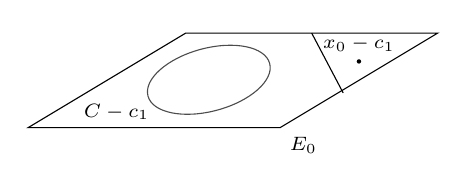
\begin{tikzpicture}[scale=0.4]
			\coordinate (A) at (-2,0);
			\coordinate (B) at (6,0);
			\coordinate (C) at (11,3);
			\coordinate (D) at (3,3);
			\draw (A) -- (B)node[below right]{$E_0$} -- (C) -- (D) -- cycle;
			\draw[rotate=15,opacity=.7](4,.5) ellipse (2cm and 1cm);
			\draw(0.8,.5)node[]{\scriptsize$C-c_1$};
			\fill(8.5,2.1)node[above]{\scriptsize$x_0-c_1$}circle(2pt);
			\draw(7,3)--(8,1.1);
		      \end{tikzpicture}
		    \end{center}
		\item  Si  $x_0-c_1\notin E_0$. No puedo usar el teorema de Hahn-Banach, porque el conjunto que quiero que separar del punto no tiene un punto interior, así que no tengo el funcional de Minkowski para separar. Pero no nos hará falta, ya que es un subespacio vectorial, yo defino una función que en el subesapcio valga cero y en el punto valga uno; Ya que, los puntos son linealmente independientes. 
 
		    Tomemos, $f:E_0+[x_0-c_1]\to \mathbb{R}$ tal que $f$ es lineal, $f_{|E_0}=0$ y $f(x_0+c_1)=1$. Entonces, 
		    $$f(c-c_1)=0<f(x_0-c_1)=1\quad \forall c\in C^i.$$
		    Esto implica que,
		    $$f(c)<f(x_0),\quad \forall c\in C^i.$$
		    No hace falta que usemos los puntos interiores, ya que el cierre de $c$ quedará en el hiperplano y ya quedará separada. De modo que, 
		    $$f(c)\leq f(x_0),\quad \forall c\in C.$$
		    Lo que extendemos a $\mathbb{R}^n$.
		    \begin{center}
		      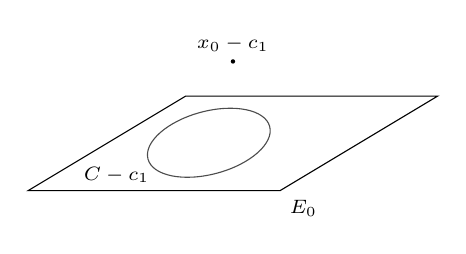
\begin{tikzpicture}[scale=0.4]
			\coordinate (A) at (-2,0);
			\coordinate (B) at (6,0);
			\coordinate (C) at (11,3);
			\coordinate (D) at (3,3);
			\draw (A) -- (B)node[below right]{$E_0$} -- (C) -- (D) -- cycle;
			\draw[rotate=15,opacity=.7](4,.5) ellipse (2cm and 1cm);
			\draw(0.8,.5)node[]{\scriptsize$C-c_1$};
			\fill(4.5,4.1)node[above]{\scriptsize$x_0-c_1$}circle(2pt);
		      \end{tikzpicture}
		    \end{center}
	    \end{enumerate}
    \end{enumerate}
    Es decir, si $C$ convexo no vacío, $C\in \mathbb{R}^n$ y $x_0\notin C$, entonces $\exists f\in \left(\mathbb{R}^n\right)^\#$ tal que $f(c)\leq f(x_0),\; \forall c\in C$.

    Ahora, el objetivo es demostrar el teorema para una separación, y como no se tiene que jugar con puntos interiores, ni con ceros. Sea $C=A-B$, como son disjuntos $0\notin C\subseteq \mathbb{R}^n$. Por lo tanto, 
    $$\exists f\in \left(\mathbb{R}\right)^\#:f(c)\leq f(0)=,\quad \forall c\in C.$$
    Lo que equivale a:
    $$f(a-b)\leq 0 \quad \forall a\in A, \forall b\in B.$$
    Utilizando la linealidad de nuevo,
    $$f(a)\leq f(b)\quad \forall a\in A, \forall b\in B.$$
    Lo que podemos tomar supremos e ínfimos quedándonos
    $$f(a)\leq \sup\left\{f(a):a\in A\right\}=r=\inf\left\{f(b):b\in B\right\}\leq f(b).$$
    Esto será verdad siempre que un conjunto este acotado. 
\end{teo}

\begin{tcolorbox}[colframe=white]
En $\mathbb{R}^n$ no hace falta encontrar puntos interiores porque la convexidad nos da puntos interiores. Si trabajamos en dimensión infinita los conjuntos convexos no tienen puntos interiores.
\end{tcolorbox}

\switchcolumn[1]*{\noindent\scriptsize
    \begin{itemize}
	\item El siguiente corolario, no es un teorema sobre $\mathbb{R}^n$, es sobre el espacio en general.
	\item La idea gráficamente sería:
	\begin{center}
	    \begin{tikzpicture}[scale=0.4,>=Triangle]
		\draw[rotate around={70:(0,0)},dashed] (0,0) ellipse (1.5cm and 1.2cm);
		\pattern[pattern=north east lines, pattern color=gray!50, rotate around={70:(0,0)}] (0,0) ellipse (1.5cm and 1.2cm);
		\draw(0,0)node[]{$C$};
		\fill (1.2,0.5) circle (4pt) node[right]{};
		\draw (.8,2.5) -- (1.6,-1.5); 
	    \end{tikzpicture}
	\end{center}
	\item Nuestro interés será encontrar una tangente que pase por el punto.
	\item Y al tomar la tangente, no me salgo del hiperplano, y el semiespacio donde queda el conjunto $C$.
	\item La tangente se ajusta al punto.
    \end{itemize}
}
\switchcolumn[0]
% ------------------- TEOREMA 2,8
\begin{teo}[Teorema del hiperplano soporte]
    Sea $C$ convexo con $\mathring{C}\neq \emptyset$ y $x_0\in \partial C$. Entonces, $\exists f\in E^\#: f(x_0)=\sup \left\{f(c):c\in C\right\}\geq f(c),\; \forall c\in \overline{C}$.

	Demostración.-\; Sea $x_0\in \mathring{C}$. Por el teorema de separación $\exists f\in E^\#$ tal que
	$$f(c)\leq f(x_0),\quad \forall c\in \mathring{C}.$$
	Lo que implica,
	$$f(c)\leq f(x_0)\quad \forall c\in \overline{C}.$$
	Por lo tanto,
	$$\sup \left\{f(c):c\in C\right\}\leq f(x_0).$$
	Como $x_0\in \overline{C}.$. Entonces,
	$$f(x_0)=\sup\left\{f(c):c\in C\right\}.$$
	Esto justifica el anterior teorema, donde el supremo o ínfimo tocarán a cualquiera de los dos conjuntos ajustándolos. 
\end{teo}

El hiperplano del gráfico de la derecha. Tiene un nombre especial, se llama \textbf{hiperplano soporte} que es lo que se definirá.

% ------------------- DEFINICIÓN 2.17
\begin{def.}
    Dado un conjunto no vacío $C\subseteq E$,  y $f\in E^\#$ al conjunto
    $$H_{c,f}=\left\{x\in E:f(x)=\sup f(c) \text{ y } c\in C\right\}$$ 
    se le llama \textbf{hiperplano soporte} a $C$ en la dirección de $f$.
\end{def.}
\begin{multicols}{2}
\begin{center}
    \begin{tikzpicture}[scale=0.4,>=Triangle]
	\draw[rotate around={70:(0,0)}] (0,0) ellipse (2cm and 1cm);
	\draw(-.5,2)node[]{$C$};
	\fill (1.05,1.4) circle (4pt) node[right]{};
	\draw[dashed,red] (.4,4) -- (1.8,-1.5)node[below]{$H_{c,f}$}; 
	\fill (-1.05,-1.4) circle (4pt) node[right]{};
	\draw[dashed,red] (-.4,-4) -- (-1.8,1.5)node[]{}; 
	\draw (1.4,5) -- (3.3,-2); 
    \end{tikzpicture}
\end{center}

Si existe $x_0\in C\cap H$, decimos que $x_0$ es un punto soporte.
\end{multicols}

\begin{tcolorbox}[colframe=white]
    Existe un saldo de la programación lineal a la programación convexa que en la programación lineal son importantes los puntos extremales, eso es porque los conjuntos son polígonos, donde puedo recuperar el polígono haciendo la envoltura convexa de los extremales. En optimización convexa, los sistemas son complejos por lo que el concepto extremal es menos importante y recobra más importancia el concepto de hiperplanos y los puntos soporte que serán el correspondiente a extremal, pero no tiene porque siempre tiene que ser extremal. 
\end{tcolorbox}

% ------------------- EJEMPLO 2.6
\begin{ejem}
    Veamos un conjunto convexo cerrado pero que no tenga punto soporte. Si tomamos 
    $$C=\left\{(x,y):y\geq e^x\right\}, \qquad f(x,y)=-y.$$
    \begin{center}
	\begin{tikzpicture}[scale=0.6]
	    \draw{(-5,0) -- (1,0)node[right]{$f$}};
	    % function e^x
	    \draw[domain=-5:1,smooth,variable=\x,blue] plot ({\x},{exp(\x)})node[right]{$e^x$};
	    \fill[pattern=north east lines, pattern color=gray!50] plot[domain=-5:1] (\x,{exp(\x)});
	    \fill (0,.95) circle (3pt) node[right]{};
	    \draw[dashed,red] (-.8,.1) -- (1,2)node[]{}; 
	\end{tikzpicture}
    \end{center}
    No hay puntos soporte. Pero lo interesante que por el teorema anterior siempre podremos construir un punto soporte. Ese soporte no tiene por que ser único.
\end{ejem}

% ------------------- EJEMPLO 2.7
\begin{ejem}
    Veamos un conjunto convexo que tenga varios puntos soporte (simultaneamente).
    \begin{center}
	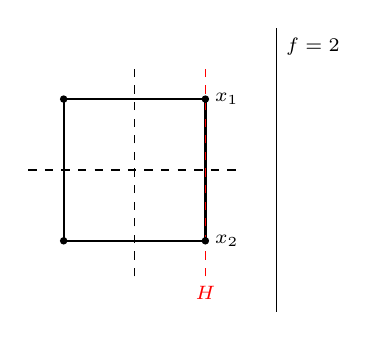
\begin{tikzpicture}[scale=0.45]
	    % draw square
	    \draw[thick] (0,0) -- (0,4) -- (4,4) -- (4,0) -- cycle;
	    % dibujar lineas dashed x e y en el origen
	    \draw[dashed] (-1,2) -- (5,2);
	    \draw[dashed] (2,-1) -- (2,5);
	    \draw[dashed,red] (4,-1)node[below]{$H$} -- (4,5);
	    \draw (6,-2) -- (6,6)node[below right]{$f=2$};
	    \fill (0,0) circle (3pt) node[right]{};
	    \fill (0,4) circle (3pt) node[right]{};
	    \fill (4,4) circle (3pt) node[right]{$x_1$};
	    \fill (4,0) circle (3pt) node[right]{$x_2$};
	\end{tikzpicture}
    \end{center}
    $$C=\left\{(x,y):\max\left\{x,y\right\}\leq 1\right\}$$
    Si un hiperplano soporte $H$ de un conjunto $C$ tiene dos puntos soporte $x_1,x_2$. Entonces, todos los puntos del $[x_1,x_2]$ son puntos soporte de $H$.
\end{ejem}

\switchcolumn[1]*{\noindent\scriptsize
	\begin{itemize}
	    \item Si tenemos conjuntos cerrados, disjuntos y al menos uno de ellos es compacto. Entonces, puedo hacer separación fuerte.
	\end{itemize}
}
\switchcolumn[0]
% ------------------- TEOREMA 2.9
\begin{teo}[Hiperplano soporte para \boldmath $\mathbb{R}^n$] Sea $C\in\mathbb{R}^n$ no vacío y convexo. Sea $x_0\in \partial C$. Entonces, existe un hiperplano soporte a $C$ de forma que $x_0$ es un punto soporte.
\end{teo}

{\color{blue}
% ------------------- EJERCICIO 2.4
\begin{ejer} Sea $C\in \mathbb{R}^n$ Sea $C\in \mathbb{R}$ cerrado y convexo. Demuestra que $C$ es la intersección de todos los semiespacios que lo contienen.

    Demostración.- Primeramente notemos que, si cualquier semiespacio $H$ tal que $C$ está completamente dentro de $H$, entonces cada punto en $C$ también pertenece a $H$. Ahora, si consideramos todos los posibles semiespacios que contienen a $C$, y tomamos su intersección, estamos buscando los puntos que son comunes a todos estos semiespacios. Dado que cada punto en $C$ pertenece a cada uno de estos semiespacios (porque cada semiespacio contiene a $C$), cada punto en $C$ también estará en la intersección de todos estos semiespacios. Por lo tanto, decimos que $C$ está contenido en la intersección de todos los semiespacios que lo contienen.

    Luego, sea un semiespacio un conjunto de la forma 
    $$H=\left\{x\in E:f(x)\leq \alpha\right\}, f\in E^\#, \alpha \in \mathbb{R}$$
    \begin{center}
	\begin{tikzpicture}[scale=0.4,>=Triangle]
	    \draw[rotate around={70:(0,0)}] (0,0) ellipse (2cm and 1cm);
	    \draw(-.5,2)node[]{$C$};
	    \fill (1.05,1.4) circle (4pt) node[right]{};
	    \draw[dashed,red] (.4,4) -- (1.8,-1.5)node[below]{$H_{c,f}$}; 
	    \fill (-1.05,-1.4) circle (4pt) node[right]{};
	    \draw[dashed,red] (-.4,-4) -- (-1.8,1.5)node[]{}; 
	    \draw (1.4,5) -- (3.3,-2); 
	\end{tikzpicture}
    \end{center}
    y sea un punto $x$ en la intersección de todos los semiespacios que contienen a $C$ pero $x\notin C$. Como $C$ es cerrado y convexo, y $x\notin C$, por el teorema de separación de Hahn-Banach, existe una función lineal $f$ y un número real $\alpha$ tal que $f(x)>\alpha$ y $f(c)\leq \alpha$ para todo $c\in C$. Esto significa que $x$ no está en el semiespacio 
    $$H=\left\{y\in \mathbb{R}^n:f(y)\leq \alpha\right\},$$ 
    lo cual es una contradicción porque asumimos que $x$ está en la intersección de todos los semiespacios que contienen a $C$. Por lo tanto, la intersección de todos los semiespacios que contienen a $C$ debe estar contenida en $C$.

    Así, demostramos que un conjunto cerrado y convexo $C$ en $\mathbb{R}^n$ es la intersección de todos los semiespacios que lo contienen.
\end{ejer}
}

% ------------------- TEOREMA 2.10
\begin{teo}
    Sean $A$ convexo y compacto, $B$ convexo y cerrado (con ejemplo de la exp que los dos sean cerrados no es suficiente), no vacíos. Tales que $A\cap B=\emptyset$. Entonces, existe $f\in \left(\mathbb{R}^n\right)^\#.$ Tal que,
    $$\sup f(a),a\in A < \inf f(b),b\in B.$$
	Demostración.-\; Calculamos 
	$$d(A,B)=\in\left\{d(a,b):a\in A, b\in B\right\}.$$
	Es decir, tomo la distancia de un punto de uno y un punto del otro y tomamos el ínfimo. Pero si no hay compacidad, no están cerrados, esos puntos no existirán. De lo contrario se alanzarán. 
	\begin{center}
	    \begin{tikzpicture}[>=Triangle,scale=.5]
		\draw[rotate=-30,opacity=.7](0,0) ellipse (1cm and 2cm);
		\draw[rotate=20,opacity=.7](4,-1.5) ellipse (1cm and 2cm);
		\fill (-.3,-.7) circle (3pt) node[below]{$a$};
		\fill (4.3,-.3) circle (3pt) node[below]{$b$};
		\draw[dashed](-.3,-.7)--(4.3,-.3);
		\fill (1.3,1) circle (3pt);
		\fill (3.12,1) circle (3pt);
		\draw[dashed](1.3,1)--(3.12,1);
	    \end{tikzpicture}
	\end{center}
	Lo que probaremos es que la $d(A,B)\neq 0$. Y al ser positiva nos permitirá encontrar un punto interior, por le cual utilizaremos el teorema de Hahn-Banach.

	La distancia lo calcularemos con la Euclideana, porque estamos en $\mathbb{R}^n$; pero podríamos calcular para cualquier norma. Es decir,
	$$d=d(A,B)=\inf\left\{\|a-b\|_2:a\in A, b\in B\right\}.$$
	(Ese ínfimo existirá, ya que está acotado por el cero inferiormente). Ahora, pueden pasar dos cosas: 
    \begin{itemize}
	\item Si $d=0$, tomamos una sucesión $\left\{a_n\right\}_n\subseteq A$ y $\left\{b_n\right\}_n \subseteq B$. De forma que,
	    $$\|a_n-b_n\|\to  d.$$
	    El hecho de que las distancias entre los puntos se acerquen a algo, no quiere decir que los puntos se acerquen a nada. Pero como $A$ es compacto, 
	    $$\left\{a_n\right\}_n\subseteq A$$
	    tiene un sucesión convergente. Y ese límite de la sucesión, como el compacto es cerrado, también está en el compacto (cerrado por lo bordes y acotado que se puede dibujar),
	    $$\left\{a_{n_k}\right\}\to a\in A. \qquad (1)$$
	    Ya que,
	    $$\|a_n-b_n\|\to 0.$$
	    Por $(1)$,  
	    \switchcolumn[1]*{\noindent\scriptsize
		La demostración de $\left\{b_{n_k}\right\}\to a$ es: Si,

		$
		\begin{array}{rcl}
		    \|b_{n_k}-a\|&\leq& \|b_{n_k}-a_{n_k}+a_{n_k}-a\|\\\\
				 &\leq& \|b_{n_k}-a_{n_k}\|+\|a_{n_k}-a\|\\\\
				 &\to& 0+0=0.
		\end{array}
		$
	    }
	    \switchcolumn[0]
	    $$\left\{b_{n_k}\right\}\to a.$$
	    Ahora, ya que $B$ es cerrado, cualquier límite de cosas $b$ están en $B$. Es decir,
	    $$a\in A\cap B.$$
	    Lo que es una contradicción, ya que $A\cap B=\emptyset$. Por lo tanto, $d\neq 0$.

	\item $d>0$. Tomamos $A'=A+\dfrac{d}{2}B_{\mathbb{R}^n}$ 
	\begin{center}
	    \begin{tikzpicture}[>=Triangle,scale=.5]
		\draw[rotate=-30,opacity=.7](0,0) ellipse (1cm and 2cm);
		\draw[rotate=20,opacity=.7](4,-1.5) ellipse (1cm and 2cm);
		\fill (-.3,-.7) circle (3pt) node[below]{$a$};
		\fill (4.3,-.3) circle (3pt) node[below]{$b$};
		\draw[dashed](-.3,-.7)--(4.3,-.3);
		\fill (1.3,1) circle (3pt);
		\fill (3.12,1) circle (3pt);
		\draw[dashed](1.3,1)--(3.12,1);
		\draw(2.2,1)node[below]{$d$};
		\draw[rotate=-30,opacity=.7,dashed](0,0) ellipse (1.9cm and 2.9cm);
		\pattern[pattern=north east lines, pattern color=gray!50, rotate around={-27:(0,0)}] (0,0) ellipse (1.9cm and 2.9cm);
	    \end{tikzpicture}
	\end{center}
	En particular, si $a\in A$. Entonces, 
	$$a+\dfrac{d}{2}B_{\mathbb{R}^n}\subseteq A'.$$
	Esto implica que, $a$ es un punto interior de $A'$. Luego, aplicamos el teorema de separación de los conjuntos, $\exists f:\mathbb{R}^n\to \mathbb{R}$ lineal, $f(a)<\inf f(b), b\in B,\; \forall a\in \interior A'$. De donde, 
	$$f(a)<\inf f(b), b\in B, \;\forall a\in A.$$
	\begin{center}
	    \begin{tikzpicture}[>=Triangle,scale=.5]
		\draw[rotate=-30,opacity=.7](0,0) ellipse (1cm and 2cm);
		\draw[rotate=20,opacity=.7](4,-1.5) ellipse (1cm and 2cm);
		\fill (-.3,-.7) circle (3pt) node[below]{$a$};
		\fill (4.3,-.3) circle (3pt) node[below]{$b$};
		\draw[dashed](-.3,-.7)--(4.3,-.3);
		\fill (1.3,1) circle (3pt);
		\fill (3.12,1) circle (3pt);
		\draw[dashed](1.3,1)--(3.12,1);
		\draw(2.2,1)node[below right]{$d$};
		\draw[rotate=-30,opacity=.7,dashed](0,0) ellipse (1.9cm and 2.9cm);
		\draw(-2.2,2)node[below right]{$B$};
		\pattern[pattern=north east lines, pattern color=gray!50, rotate around={-27:(0,0)}] (0,0) ellipse (1.9cm and 2.9cm);
		\draw[red](2.15,-3)--(2.25,4);
	    \end{tikzpicture}
	\end{center}
	Como $A$ es compacto, existe 
	$$a_0\in A:f(a_0)=\sup f(a),a\in A.$$ 
	Entonces,
	$$f(a)\geq f(a_0)<\inf \left\{f(b)\right\},b\in B.$$
    \end{itemize}
\end{teo}

\section{Conos duales }
\begin{tcolorbox}[colframe=white]
    Los conos se establecen para ordenes en $\mathbb{R}^n$ que son multicriterio. Donde hablaremos de conos duales, que es importante ya que cuando hagamos optimización y nuestro dominio sea un cono, lo dualizaremos, cuando hagamos el dual del problema, el cono que nos saldrá es el cono dual. Entonces necesitamos saber como es el cono dual para poder trabajar con el cono dual.
\end{tcolorbox}

\switchcolumn[1]*{\noindent\scriptsize
\begin{center}
    \begin{tikzpicture}[>=Triangle,scale=.5]
	\draw[pattern=north east lines, pattern color=gray!40, draw=white,rotate around={0:(0,0)}] (0,0) -- (5cm,-1.1) -- (-1,4.5cm) -- cycle;
	\draw[dashed](0,0)--(-1,4.5);
	\draw[dashed](0,0)--(5,-1);
	\draw(-1,2)node[below left]{$K$};
	\draw[pattern=north west lines, pattern color=red!20, draw=white,rotate around={0:(0,0)}] (0,0) -- (5cm,1.1) -- (1,4.5cm) -- cycle;
	\draw[red](0,0)--(1,4.5);
	\draw[red](0,0)--(5,1);
	\draw[red](3.5,3.5)node[below left]{$K^*$};
	\draw[blue!50](-.1,.43)--(.4,.56)--(.53,.1);
	\draw[green](.1,.5)--(.6,.43)--(.49,-.12);
    \end{tikzpicture}
\end{center}
}
\switchcolumn[0]
Partimos de 
$$K\in \mathbb{R}^n$$
que es un cono. Y a partir de aquí se define su cono dual como:
$$
\begin{array}{rcl}
    K^*&=&\left\{y\in \mathbb{R}^n: y^T x\geq 0,\forall x\in K\right\}\\\\
       &=&\left\{y\in \mathbb{R}^n: \langle y,x\rangle\geq 0,\forall x\in K\right\}.
\end{array}
$$

Lo que tenemos que hacer es tomar lineas perperdiculares a las dos lineas que forman el cono, dando nos da un cono dual. 

% -------------------- EJEMPLO 2.8
\begin{ejem}
    Si $\|\cdot\|$ es una norma en $\mathbb{R}^n$. Entonces,
    $$K=\left\{(x,t)\in \mathbb{R}^n:\|x\|\leq t\right\}\subseteq \mathbb{R}^{n+1}$$
    (En realidad es cómo representar la gráfica de la función de la norma, y tomar el cono que se forma; es decir, una dimensión más).
\end{ejem}

\switchcolumn[1]*{\noindent\scriptsize
    Tenemos una norma en espacio de Banach, en espacio normado. Cuando hacemos el dual, cuando vemos a $\mathbb{R}^n$ como aplicaciones lineales y continuas, entonces nos sale una norma nueva, esa norma se llama norma dual, que es importante.
}
\switchcolumn[0]\noindent
% --------------------- DEFINICIÓN 2.18
\begin{def.}
    La \textbf{norma dual} de $\left(\mathbb{R}^n,\|\cdot\|\right)$. Y si define como:
    $$\|y\| = \sup\left\{\langle y,x\rangle: x\in B_{\|\cdot\|}\right\}.$$
\end{def.}

\begin{tcolorbox}[colframe=white]
La definición de cono dual se lleva bien con la definición de arriba y el resultado sería esta proposición: 
\end{tcolorbox}

\switchcolumn[1]*{\noindent\scriptsize
    Si utilizamos el cono $K=\left\{(x,t)\in \mathbb{R}^n:\|x\|\leq t\right\}\subseteq \mathbb{R}^{n+1}$, que \textbf{se usa mucho en optimización} y dualizamos lo que tendremos es el cono dual de la proposición 2.2 que no es más la que define a norma dual. Es decir, tomaríamos la norma, la dibujaríamos y aplicaríamos todo lo que está por encima.  
}
\switchcolumn[0]\noindent
% --------------------- PROPOSICIÓN 2.2
\begin{proposicion}
    Si tomamos $\left\{(x,t):\|x\|\leq t\right\}^*=\left\{(y,s):\|y\|^*\leq s\right\}.$

	Demostración.-\; Tomemos un punto de uno de los lados y demostraremos que ese punto ahí, si y sólo si está en el otro. Para ello, sea 
	$$(y,s)\in \left\{(y,s):\|y\|^*\leq s\right\}.$$
	De donde,
	$$\|y\|^*\leq s.$$
	Utilizando la definición 2.18 de norma dual se tiene,
	$$\sup\left\{\langle y,x\rangle: x\in B_{\|\cdot\|}\right\}\leq s.$$
	Luego, por el producto escalar,
	$$y^Tx\leq s,\;\forall x\in B_{\|\cdot\|}.$$
	El hecho de que $x$ esté en la bola, me permitirá tomar los múltiplos de $x$. En otras palabras si yo multiplico $x$ por algún número. Entonces,
	\switchcolumn[1]*{\noindent\scriptsize
	    Demostremos que $ y^Tx\leq s,\;\forall x\in B_{\|\cdot\|}$ es equivalente a $y^Tx\leq s,\;\forall x\in \mathbb{R}^n$. Dado $x\in \mathbb{R}^n, t\geq \|x\|$. Entonces, $\dfrac{x}{t}\in B_{\mathbb{R}^n}$
	}
	\switchcolumn[0]\noindent
	$$y^Tx\leq st,\;\forall x\in \mathbb{R}^n,\;\forall t\geq \|x\|.$$
	Ahora, vemos que el espacio en $\mathbb{R}^n$ es simétrico. Es decir, para cualquier $y$, tenemos  $-y$. Por lo que,
	$$-y^Tx\leq st,\;\forall x\in \mathbb{R}^n,\;\forall t\geq \|x\|.$$
	Lo que es equivalente a decir que,
	$$
	\begin{array}{rcll}
	    st+y* Tx&\geq& 0,&\forall x\in \mathbb{R}^n,\;\forall t\geq \|x\|\\\\
	    \langle (y,s),(x,t)\rangle&\geq& 0,& \forall (x,t)\in K.
	\end{array}
	$$
	Por lo tanto por definición,
	$$(y,s)\in K^*.$$
\end{proposicion}

\begin{tcolorbox}[colframe=white]
Estos conos duales tiene una serie de propiedades interesantes ya que nos permitirá hacer order.
\end{tcolorbox}

\switchcolumn[1]*{\noindent\scriptsize
    \begin{itemize}
	\item Apuntado significa que no puede tener un vector y su opuesto. El único vector opuesto es el cero. Si $y,-y\in K^* \Rightarrow y=0$.
	\item Tener punto interior y ser apuntado, son propiedades duales.
	\item La 5) nos dice que si realizo la operación dos veces lo que consigo es cerrar.
    \end{itemize}
}
\switchcolumn[0]\noindent
% -------------------- PROPIEDAD 2.4
\begin{prop}
    Sea $K$ un cono en $\mathbb{R}^n$.
    \begin{enumerate}[1)]
	\item $K^*$ es un cono convexo y cerrado.
	\item $K_1\subseteq K_2\Rightarrow K_2^*\subseteq K_1^*$.
	\item $\mathring{R}\neq\emptyset \Rightarrow K^*$ apuntado o punteagudo.
	\item $\overline{K}$ y es apuntado $\Rightarrow K^*$ tiene interior  no vacío.
	\item $K^{**}=\overline{\co{K}}$.
    \end{enumerate}
\end{prop}

\switchcolumn[1]*{\noindent\scriptsize
	\begin{itemize}
	    \item Por propio, se refiere a que podemos tener un orden. En otras palabras, que sea apuntado, que tuviese un punto interior, que sea convexo, etc.
	\end{itemize}
}
\switchcolumn[0]\noindent
%-------------------- COROLARIO 2.1
\begin{cor}
    Si $K$ es propio. Entonces, $K^*$ es propio.
\end{cor}

\end{paracol}






\chapter{Funciones convexas}

\begin{paracol}{2}

\section{Propiedades básicas}

\subsection{Definición}

Por defecto el dominio será $\mathbb{R}^n$, con la peculiaridad que tomaremos el valor más infinito.
Y llamaremos dominio efectivo, al conjunto donde esa función toma valores finitos.

\begin{tcolorbox}[colframe=white]
    Para empezar a definir una función convexa, necesitaremos que el dominio sea un conjunto convexo. 
\end{tcolorbox}

\switchcolumn[1]*{\noindent\scriptsize
	\begin{itemize}
	    \item La imagen de la combinación convexa, es  menor igual que las combinación convexa de las imágenes.
	    \item Importante que sea para todo $x$ e $y$ en el dominio.
	    \item Necesito que el conjunto sea convexo. Si tomas dos puntos $(x,y)$ cualesquiera, olvídate de todo el conjunto y sólo quédate con el segmento. 
	    \item La definición geométricamente, nos dice que para cualquier punto del segmento la imagen de la función se queda por debajo de la cuerda.
	\end{itemize}
}

\switchcolumn[0]\noindent
%-------------------- DEFINICIÓN 3.1
\begin{def.}[Función convexa] $f:\mathbb{R}^n\to \mathbb{R}$ tal que $\text{Dom}(f)\subseteq \mathbb{R}^n$ convexo, y
    $$f\left[tx+(1-t)y\right]\leq tf(x)+(1-t)f(y), \text{ para } 0\leq 1.$$
\end{def.}

    \begin{multicols}{2}
	\begin{center}
	    \begin{tikzpicture}[>=Triangle,scale=.5]
		\draw[rotate=40,opacity=.7] (0,0) ellipse (1.5cm and 2cm);
		\draw(0,2)node[above]{\tiny$\text{Dom}(f)\in \mathbb{R}^n$};
		\draw[blue](-1,.5)--(.9,-.5);
		\fill(-1,.5)node[below]{\tiny $x$}circle(2pt);
		\fill(.9,-.5)node[below]{\tiny $y$}circle(2pt);
		\node[rotate=-25,above, red] at (.1,0) {\tiny$tx+(1-t)y$};
	    \end{tikzpicture}
	\end{center}
	\begin{center}
	    \begin{tikzpicture}[>=Triangle,scale=.4]
		\draw[dashed,gray!50](0,-5)--(0,0);
		\draw[dashed,gray!50](6,-5)--(6,-1);
		\draw[dashed,gray!50](2.5,-.5)--(2.5,-5);
		\draw[blue,rotate=-10,opacity=.7](0,0) arc (200:340:3.2cm);
		\node[red,rotate=-8] at (2.5,.6)[below]{\tiny$tf(x)+(1-t)f(y)$};
		\draw[rotate=-10,red](0,0)--(6,0)node[below]{};
		\node[blue] at (2.7,-2.5)[below]{\tiny$f\left(tx+(1-t)y\right)$};
		\draw[](0,-5)--(6,-5)node[below]{};
		\foreach \x/\xtext/\y in {0/$\tiny x$/-.1,2.5/$\tiny tx+(1-t)y$/-.1,6/$\tiny y$/-.1}
		{
		\draw (\x,-5.2) -- (\x,-4.8) node[below,yshift=\y cm] {$\xtext$};
		}
	    \end{tikzpicture}
	\end{center}
    \end{multicols}

% -------------------- DEFINICIÓN 3.2
\begin{def.}[Función Cóncava] Satisface la desigualdad opuesta de convexa. Es decir,
    \begin{center}
	$f$ cóncava $\Leftrightarrow$ $-f$ convexa.
    \end{center}
\end{def.}

\switchcolumn[1]*{\noindent\scriptsize
	\begin{itemize}
	    \item ¿Es posible que una función sea cóncava y convexas a la vez?. Si, Una función es cóncava y convexa a la vez, si y sólo si es afín (la imagen es un subspacio lineal, es una linea que pasa por cualquier punto.). Las rectas en una dimensión, los planos, etc. 
	\end{itemize}
}
\switchcolumn[0]\noindent
\begin{tcolorbox}[colframe=white]
    La convexidad es un concepto muy fuerte, que es una propiedad de todo un conjunto, ya que lo cumplen todos los pares de puntos, pero a la larga es un concepto uno-dimensional. Es decir, hay dos puntos, tomamos la linea que une los dos puntos y estudiamos conexidad en una variable en esa recta. 
\end{tcolorbox}


\subsection{Definiciones más fuertes}

Muchas veces veremos que la función no es estrictamente convexo.


\switchcolumn[1]*{\noindent\scriptsize
	\begin{itemize}
	    \item La idea será que no haya segmentos; es decir, que no haya igualdad en la definición de convexa.
	\end{itemize}
}
\switchcolumn[0]\noindent
% -------------------- DEFINICIÓN 3.3
\begin{def.}[Estrictamente Convexa] $f$ es estrictamente convexa si
	$$f\left[tx+(1-t)y\right]< tf(x)+(1-t)f(y)$$
	para $x\neq y$ y $0<t<1$. Es decir, $f$ es convexa y tiene mayor curvatura que una función lineal.
\end{def.}

\switchcolumn[1]*{\noindent\scriptsize
	\begin{itemize}
	    \item No sólo pediremos que que no tenga segmentos si no también que se curve cómo un polinomio de grado dos.
	\end{itemize}
}
\switchcolumn[0]\noindent
% -------------------- DEFINICIÓN 3.4
\begin{def.}[Fuertemente Convexa] Con parámetro $m>0$:
    $$f-\dfrac{m}{2}\|x\|^2_2$$
    es convexa. Es decir, $f$ es al menos tan convexa como una función cuadrática.
\end{def.}

\switchcolumn[1]*{\noindent\scriptsize
	\begin{itemize}
	    \item Si tenemos una función fuertemente convexa es estrictamente convexa y una estrictamente convexa es convexa. Pero ninguna de estas implicaciones es cierta hacia atrás. Es decir, hay funciones convexas que no son estrictamente convexas, y hay funciones estrictamente convexas que no son fuertemente convexas.
	\end{itemize}
}
\switchcolumn[0]\noindent
\begin{tcolorbox}[colframe=white]
    Claramente:
    $$\beta-\text{convexa}\Rightarrow \text{Estrictamente Convexa} \Rightarrow \text{Convexa}.$$
    (Análogamente para funciones cóncavas).
\end{tcolorbox}

\begin{tcolorbox}[colframe=white]
    Es conveniente considerar que nuestras funciones están definidas en todo el espacio. Así, cuando tengamos una función $f$ cuyo dominio es un subconjunto de $\mathbb{R}^n$, identificaremos $f$ con su extension.
\end{tcolorbox}



\subsection{Propiedades clave: Epígrafo}


Sea $f:\mathbb{R}^n\rightarrow\mathbb{R}$, se define una gráfica como:
$$G(f)=\left\{(x,f(x)):x\in\text{Dom}(f)\right\}\subseteq \mathbb{R}^n\times \mathbb{R}.$$
Por lo que definimos lo siguiente:


\switchcolumn[1]*{\noindent\scriptsize
	\begin{itemize}
	    \item Básicamente el epígrafo será los puntos que están por encima de la función.
	    \item Si ahora, tomo el punto de conjuntos por encima de la gráfica, ese conjunto es convexo. Por lo que, todo lo que sabemos sobre conjuntos convexos, lo podemos aplicar a funciones convexas trasladando el concepto conjuntista al concepto funcional.
	\end{itemize}
}
\switchcolumn[0]\noindent
%------------------- DEFINICIÓN 3.5
\begin{def.}[Epígrafo]
    $$\text{Epi}(f)=\left\{(x,t):x\in \text{Dom}(f),t\geq f(x)\right\}\subseteq \mathbb{R}^n\times \mathbb{R}.$$
    \begin{center}
	\begin{tikzpicture}[>=Triangle,scale=.5]
	    \draw[dashed,gray!50](0,-1)--(0,5);
	    \draw[dashed,gray!50](6,-1)--(6,5);
	    \draw[dashed,gray!50](4,-1)--(4,1);
	    \draw[dashed,gray!50](4,1)--(6,1);
	    \fill[pattern=north east lines, pattern color=gray!50] (0,5) -- plot[domain=0:6] (\x,{1/16*\x*\x}) -- (6,5) -- cycle;
	    \node at (3,3) {$E$};
	    \draw(6,1)node[right]{\scriptsize$f(x)$};
	    \draw[domain=0:6,smooth,variable=\x,blue] plot ({\x},{\x*\x/16});
	    \fill[blue](4,1) circle (3pt);
	    \node[above,rotate=20,blue] at (4,1) {\scriptsize$(x,f(x))$};
	    \draw[](0,-1)--(6,-1)node[below]{};
	    \foreach \x/\xtext/\y in {0/a/-.1,4/x/-.1,6/b/-.1}
	    {
	    \draw (\x,-1.2) -- (\x,-.8) node[below,yshift=-.2 cm] {\scriptsize$\xtext$};
	    }
	\end{tikzpicture}
    \end{center}
\end{def.}

\switchcolumn[1]*{\noindent\scriptsize
	\begin{itemize}
	    \item Podremos tratar al hipógrafo como el epígrafo de la función $-f$.
	\end{itemize}
}
\switchcolumn[0]\noindent
%------------------- DEFINICIÓN 3.6
\begin{def.}[Hipógrafo]
    $$\text{Hipo}(f)=\left\{(x,t):x\in \text{Dom}(f),t\leq f(x)\right\}\subseteq \mathbb{R}* n\times \mathbb{R}.$$
\end{def.}

%------------------- TEOREMA 3.1
\begin{teo} $f$ es convexa sii $\text{Epi}(f)$ es convexo.
    \switchcolumn[1]*{\noindent\scriptsize
    }
    \switchcolumn[0]\noindent
    Demostración.-\; $\left.\Rightarrow\right]$ Suponemos que $f$ es convexa, por lo que $\text{dom}(f)$ efectivo es convexo. Ahora, lo que quiero demostrar es que el hepígrafo es un conjunto convexo. Para ello, tomamos dos puntos cualesquiera del epígrafo,
	$$(x,t),(y,s)\in \text{Epi}(f),\; \lambda \in \left[0,1\right].$$
    \begin{center}
	\begin{tikzpicture}[>=Triangle,scale=.6]
	    \draw[](-3.5,-1)--(4.2,-1)node[below]{};
	    \draw[domain=-3.5:4.2,smooth,variable=\x,blue] plot ({\x},{\x*\x/3});
	    \fill[pattern=north east lines, pattern color=gray!20] (-3.5,4.1) -- plot[domain=-3.5:4.2] (\x,{1/3*\x*\x});
	    \fill[draw](-2.1,3.5)node[above left]{\scriptsize$(x,t)$} circle (2pt) -- (0,3.915) circle (2pt)node[above,rotate=10]{\scriptsize$\lambda t+(1-\lambda) s$} -- (2.74,4.5)node[above]{\scriptsize$(y,s)$} circle (2pt);
	    \fill[draw](-2.1,1.5)node[left]{\scriptsize$a$} circle (2pt) -- (0,1.915)node[below left]{\scriptsize$c$} circle (2pt) -- (2.74,2.5)node[right]{\scriptsize$b$} circle (2pt);
	    \draw[dashed,gray](-2.1,3.5)--(-2.1,-1);
	    \draw[dashed,gray](2.74,4.5)--(2.74,-1);
	    \draw[dashed,red](0,3.915)--(0,-1);
	    \fill[draw](0,0) circle (2pt)node[below right]{\scriptsize$d$};
	    \foreach \x/\xtext/\y in {-2.1/ x/-.1,0/\lambda x +(1-\lambda)y/-.1,2.74/ y/-.1}
	    {
	    \draw (\x,-1.2) -- (\x,-.8) node[below,yshift=-.2 cm] {\scriptsize$\xtext$};
	    }
	\end{tikzpicture}
    \end{center}
    Por definición sabemos que el segmento que une a los puntos $a$ y $b$ está por encima de $f$. Y dado que $c$ esta por encima de $d$. Entonces, $\lambda (x,t) + (1-\lambda)(y,s)$ esta por encima de $d$. Es decir, 
    $$\lambda (x,t) + (1-\lambda)(y,s)\in \text{Epi}(f).$$
    Esto es equivalente a,
    $$\left[\lambda x + (1-\lambda)y,\lambda t + (1-\lambda)s\right]\in \text{Epi}(f).$$
    Escribiendo en términos de punto, se tiene
    $$\lambda t + (1-\lambda)s\geq f\left(\lambda x + (1-\lambda)y\right).$$
    Probemos ahora que esta desigualdad es cierta. Por lo tanto por convexidad:
    $$f\left[\lambda x + (1-\lambda) y\right]\leq \lambda f(x) + (1-\lambda)f(y)\leq \lambda t+(1-\lambda)s.$$
    La segunda desigualdad es dado porque $(x,t)$ está en el epígrafo; Y por definición, $f(x)\leq t$ y $f(y)\leq s$. 
    \switchcolumn[1]*{\noindent\scriptsize
	\begin{itemize}
	    \item Si tomo un conjunto convexo y lo proyecto me sale también convexo. Si hago la proyección a una de las coordenadas me sale convexo. Eso me será necesario ya que en la definición que la función es convexa, lo primero que tengo que demostrar es que el dominio es convexo. 
	    \item En resumen, si el conjunto es convexo, el dominio efectivo es convexo.
	\end{itemize}
	}
    \switchcolumn[0]\noindent
    $\left.\Leftarrow\right]$ $\text{Epi}(f)$ es convexo. Sean $x,y\in \text{Dom}(f)$. Lo primero que tenemos que demostrar es que el dominio es convexo, debido a que es convexo por ser la proyección a la primera coordenada de un convexo. Luego, sea $\lambda \in (0,1)$, nos preguntamos si:
    $$f\left[\left(\lambda x + (1-\lambda)y\right)\leq \lambda f(x) + (1-\lambda)f(y)\right].$$
    Ahora, lo que quiero probar es si el conjunto es convexo. Entonces, la función es convexa. Por lo que aplicaremos la definición de convexidad del conjunto pero solo a los puntos de la recta del medio del gráfico de arriba que se intesectan con la función. Es decir, 
    $$x\in \text{Dom}(f) \Rightarrow (x,f(x))\in \text{Epi}(f).$$
    y 
    $$y\in \text{Dom}(f) \Rightarrow (y,f(y))\in \text{Epi}(f).$$
    Pero, sabemos que el epígrado es una función convexas. Que implica,
    $$\lambda (x,f(x)) + (1-\lambda)(y,f(y))\in \text{Epi}(f).$$
    Transformado esta última ecuación a vector único, se tiene
    $$\left[\lambda x + (1-\lambda)y,\lambda f(x) + (1-\lambda)f(y)\right]\in \text{Epi}(f).$$
    Por lo tanto,
    $$\lambda f(x) + (1-\lambda)f(y)\geq f\left[\lambda x + (1-\lambda)y\right].$$
    De esta manera queda demostrado el teorema.
\end{teo}

% -------------------- TEOREMA 3.2
\begin{teo} $f$ es cóncava sii $hipo(f)$ es convexo.

\end{teo}

\begin{tcolorbox}[colframe=white]
    El siguiente teorema es importante en optimización práctica. Ya que, al querer encontrar un sólo mínimo muchas veces damos vueltas, cuando hay un argumento muy sencillo si sabemos que la función es convexa. Entonces, hay funciones de forma natural son convexas y que cuando encontramos un extremo local (aplicando Fermat, Lagrange, Gradiente=0); encontramos un extremo global que no hace falta que sea mínimo, por lo tanto la función es convexas es el mínimo global. 
\end{tcolorbox}

% -------------------- TEOREMA 3.3
\begin{teo} Sea $f$ convexa, $x_0$ un mínimo local de $f$. Entonces, $x_0$ es un mínimo global.

    Demostración.-\; Sea $\delta>0$ tal que $f(z)\geq f(x_0),\; \forall z\in B(x_0,\delta)\cap Dom$. Lo que quiero demostrar es que la desigualdad dada, no sólo es cierta para todos los puntos de la bola si no para todos los puntos cualquiera. Así, que tomamos un $y\in Dom\backslash B(x_0,\delta)$; la idea será:
    \begin{center}
	\begin{tikzpicture}[>=Triangle,scale=.6]
	    \draw[rotate=-60,opacity=.7](0,0) ellipse (1.5cm and 3cm);
	    \draw[opacity=.7](-1,-.5) circle (25pt);
	    \fill (-1,-.5) circle (2pt); 
	    \draw[->] (-1,-.5)node[below]{\scriptsize$x_0$} -- (-1.5,.25)node[yshift=-10]{\scriptsize$\delta$};
	    \fill (2,1.2) circle (2pt)node[below right]{\scriptsize$y$};
	    \draw (-1,-.5) -- (2,1.2);
	    \fill (-.24,-.08) circle (2pt)node[below right]{\scriptsize$z$};
	\end{tikzpicture}
    \end{center}
    ¿Cuál es la idea para demostrar que la $f(y)$ es necesariamente mayor o igual que cero $f(x_0)$?. Si lo pensamos en una dimensión tendríamos:
    \begin{center}
	\begin{tikzpicture}[>=Triangle,scale=.5]
	    \tikzstyle{every node}=[font=\scriptsize]
	    \draw[](-2,0)--(6,0)node[below]{};
	    \draw[domain=-1:1,smooth,variable=\x,blue] plot ({\x},{\x*\x+2});
	    \draw[dashed,fill](0,0)--(0,2)circle (2pt);
	    \draw[dashed](0,2)--(5,2);
	    \fill (4,1.5) circle (3pt);
	    \draw[red](0,2)--(4,1.5);
	    \draw[dashed,fill](1,0)--(1,3)circle (2pt);
	    %crear flecha curva
	    \draw[->,opacity=.3] (2,1.8) to [out=0,in=220] (4,3)node[above,rotate=-30]{Violará la definción de convexidad};
	    \foreach \x/\xtext/\y in {0/x_0/0, 1/z/0 ,4/y/0}
	    {
	    \draw (\x,.1) -- (\x,-.1) node[below,yshift=-1mm] {$\xtext$};
	    }
	    \draw[>={Bracket[width=3mm,line width=.5pt,length=.5mm]},<->] (-1, 0) -- (1, 0);
	\end{tikzpicture}
    \end{center}

    \switchcolumn[1]*{\noindent\scriptsize
	\begin{itemize}
	    \item $x_0$ se que está en la bola, ya que si calculamos la distancia de $\frac{\delta}{\|x_0-y\|}$ a $x_0$ nos saldrá $\delta$ ($B(x_0,\delta)$) y además está en el Dominio $Dom$ por que es convexo. Cómo $x_0$ e $y$ están $z$ está.
	    \item Para no cometer ningún un error estricto de las desigualdades será $y\in Dom\backslash B(x_0,\delta)$. Porque ya se lo que pasa con los puntos de la bola, tomo un punto que no este en la bola, si el punto no está en la bola su distancia es más grande que $\delta$, entonces $\frac{\|y-x_0\|-\delta}{\|y-x_0\|}x_0\geq 0$, suman $1$. Es decir, es una combinación convexa.
	\end{itemize}
    }
    \switchcolumn[0]\noindent
    Definimos $z$ como:
    $$z=x_0+\dfrac{\delta}{\|x_0-y\|}(y-x_0)\in Dom(f)\cap B(x_0,\delta).$$
    Dado que $z$ está en un segmento se puede escribir como la combinación convexa de $x_0$ e $y$. Es decir,
    $$z=\dfrac{\|y-x_0\|-\delta}{\|y-x_0\|}x_0+\dfrac{\delta}{\|y-x_0\|}y.$$
    Luego, Utilizamos la definición de convexidad de una función y veamos que la propiedad de la conexidad me permite trasladar una propiedad local; es decir, me permite llevar una propiedad que pasa cerca al punto tan lejos como quiera. 
    $$f(x_0)\leq f(z)\leq \dfrac{\|y-x_0\|-\delta}{\|y-x_0\|}f(x_0)+\dfrac{\delta}{\|y-x_0\|}f(y).$$
    Ahora, dejo aislada $f(y)$ de forma que
    $$\dfrac{\delta}{\|y-x_0\|}f(y)\geq \dfrac{\delta}{\|y-x_0\|}f(x_0) \quad \Rightarrow \quad f(y)\geq f(x_0).$$
    En resumen, si tengo un extremo local, entonces la imagen de los puntos que están lejos no pueden estar por debajo de ese extremo local, ya que nos llevaría una contradicción en el punto $z$.
\end{teo}


\subsection{Condición de primer orden}

\begin{tcolorbox}[colframe=white]
    El siguiente teorema es la generalización para la funciones diferenciables y toda la parte teórica de funciones convexas y la parte de dualidad nos hará convencer de que ser convexa aunque no tenga diferenciabilidad será del siguiente estilo:
    $$f(y)\geq f(x_0)+\nabla f(x_0)^T(y-x_0).$$
    \begin{center}
	\begin{tikzpicture}[>=Triangle,scale=.5]
	    \tikzstyle{every node}=[font=\scriptsize]
	    \draw[](-4,0)--(4,0)node[below]{};
	    \draw[domain=-2.5:2.5,smooth,variable=\x,blue] plot ({\x},{1/2*\x*\x+2});
	    \draw[dashed,fill](1.5,0)--(1.5,3.1)circle (2pt);
	    \foreach \x/\xtext/\y in {1.5/x_0/0}
	    {
	    \draw (\x,.1) -- (\x,-.1) node[below,yshift=-1mm] {$\xtext$};
	    }
	    \draw[domain=-1:3,smooth,variable=\x,red] plot ({\x},{1.5*(\x-1.5)+3.1})node[right]{$f(x)+f'(x_0)(x-x_0)=y$};
	    \draw[dashed,fill](-0.566,0)--(-0.566,2.16)circle (2pt) -- (-3,2.16)node[left]{$f(y)$};
	\end{tikzpicture}
    \end{center}
    $G(f)$ queda por encima de las rectas tangentes.
\end{tcolorbox}
\;\\
Empecemos demostrando el siguiente lema que nos asegurará que estará definida para algo pequeño.

% -------------------- Lema 3.1
\begin{lema} Para todo $x\in \mathbb{R}^n$, la función $h_x(t)=\dfrac{f(x_0+tx)+f(x_0}{t}$, es monótona no decreciente para $t>0$.

    Demostración.-\; Fijamos $0<t<s,\; x\in \mathbb{R}^n$. Lo que quiero probar es que la función pendiente $h(t)$ cuando la evalúe en $t$ saldrá menor o igual cuando la evalúo en $s$. De manera geométrica se ve de la siguiente manera:
    \begin{center}
	\begin{tikzpicture}[>=Triangle,scale=.45]
	    \tikzstyle{every node}=[font=\scriptsize]

	    \draw[](-4,0)--(5,0);
	    \draw[domain=-3:3,smooth,variable=\x,blue] plot ({\x},{1/4*\x*\x+2});

	    \foreach \x/\xtext/\y in {-2/x_0/0,-.5/x_0+tx/0,1.8/x_0+sx/0}
	    {
	    \draw (\x,.1) -- (\x,-.1) node[below,yshift=-1mm] {$\xtext$};
	    }

	    \draw[dashed,fill](-2,0)--(-2,3)circle (2pt);
	    \draw[dashed,fill](-0.5,0)--(-0.5,2.05) circle (2pt);
	    \draw[dashed,fill](1.8,0)--(1.8,2.8) circle (2pt);

	    \draw[red](-0.5,2.05)--(-2,3)--(1.8,2.8);
	\end{tikzpicture}
    \end{center}

    En sí, lo que vamos a demostrar es que $x_0+tx$ es una combinación convexa de $x_0$ y $x_0+tx$. Por lo que,
    $$x_0+tx=\dfrac{t}{s}(x_0+sx)+\dfrac{s-t}{s}x_0.$$
    De donde, por definición de convexidad
    $$f(x_0+tx)\leq \dfrac{t}{s}f(x_0+sx)+\dfrac{s-t}{s}f(x_0).$$
    Ahora, compararemos $h_x(t)$ y $h_x(s)$, de manera que
    $$
    \begin{array}{rcl}
	h_x(t)&=&\dfrac{f(x_0+tx)-f(x_0)}{t}\\\\
	   &\leq& \dfrac{\dfrac{t}{s}f(x_0+sx)-\dfrac{t}{s}f(x_0)}{s}\\\\
	   &=&\dfrac{1}{s}\left[f(x_0+sx)-f(x_0)\right]\\\\
	   &=&h_x(s).
    \end{array}
    $$
    Luego, $h_x(t)\leq h_x(s).$
\end{lema}


% -------------------- Teorema 3.4
\begin{teo} si $f$ es diferenciable. Entonces, $f$ es convexa si y sólo si, $dom(f)$ es convexo, y
$$f(y)\geq f(x_0)+\nabla f(x_0)^T(y-x_0).$$
para todo $x,y\in D(f)$.
\switchcolumn[1]*{\noindent\scriptsize
    \begin{itemize}
	\item La ecuación nos dirá que $f(y)$ está controlada por debajo por una ecuación afín, se le llama también subestimador afín.
	\item Que la función sea convexa nos dice que el dominio es convexo.
    \end{itemize}
}
\switchcolumn[0]\noindent
    Demostración.-\; $\left.\Rightarrow\right]$. Sabemos que $f$ es convexa y diferenciables.  En la definición de diferenciable, para poder decir que es diferenciable en un punto, necesito que ese punto sea interior, observemos también que $D$ es abierto, por lo que empezamos suponiendo que $x_0\in \mathring{D}$. 

    Por el lema 3.1,  $x_0\in\mathring{D}$ en $h_x$ está bien definida al menos en $[0,\delta)$ para cierto $\delta_x>0$, que depende de $x$.

    Ahora, como $f$ es diferenciable, podemos calcular las derivadas direccionales,
    $$D_{(y-x_0)}f(x_0)=\nabla f(x_0)^T\cdot (y-x_0).$$
    Pero al mismo tiempo tengo la definición de derivada direccional,
    $$D_{y-x_0}f(x_0)=\lim_{t\to 0* +}h_{(y-x_0)}(t).$$
    (Dado que es diferenciable, el límite existe por la derecha e izquierda, por lo que me puedo permitir ir sólo por la derecha). 

    \switchcolumn[1]*{\noindent\scriptsize
	\begin{itemize}
	    \item Cómo $h_{(y-x_0)}(t)\leq h_{(y-x_0)}(1)$ son menores o iguales que el que es mayor, todos los $t$ cuando se acercan a $0$ son menores que $1$, luego $h_{(y-x_0)}(t)$ son menores o iguales que que la imagen de $1$, y el límite también.
	    \item En este caso, si $y$ está en el dominio, vemos que la función está definida hasta el $1$ y el $\delta$ es este caso es más grande. Por lo tanto, puedo trabajar con ese $1$.
	\end{itemize}
    }
    \switchcolumn[0]\noindent
    Después, utilicemos la monotonía, del lema 3.1,
    $$
    \begin{array}{rcl}
	\displaystyle\lim_{t\to 0^+}h_{(y-x_0)}(t) &\leq& h_{(y-x_0)}(1)\\\\
						   &=& \dfrac{f(x_0+(y-x_0))-f(x_0)}{1}\\\\
						   &=& f(y)-f(x_0).
    \end{array}
    $$
    
    De donde tenemos,
    $$f(y)\geq f(x_0) \nabla f(x_0)^T(y-x_0) \quad \forall y\in D,\; \forall x_0\in D.$$

    $\left.\Leftarrow\right]$. Supongamos que $D$ es convexo y que
    $$f(y)\geq f(x)+\nabla f(x)^T(y-x), \quad \forall x,y\in D.$$

    \switchcolumn[1]*{\noindent\scriptsize
	\begin{center}
	    \begin{tikzpicture}[>=Triangle,scale=.5]
		\tikzstyle{every node}=[font=\scriptsize]

		\draw[dashed,gray!50](-2,-1)--(-2,5);
		\draw[dashed,gray!50](6,-1)--(6,5);

		\def\funcA{2+cos(deg(\x+2))}
		\def\funcB{-\x/3+1.3}
		\def\funcC{\x/2+.28}

		\draw[domain=-2:6,smooth,variable=\x,red] plot ({\x},{\funcA});

		\fill[pattern=north east lines, pattern color=gray!35] (-2,5) -- plot[domain=-2:6] (\x,{\funcB}) -- (6,5) -- cycle;
		\draw[domain=-2:6,smooth,variable=\x,blue] plot ({\x},{\funcB});

		\draw[domain=-2:6,smooth,variable=\x,blue!50] plot ({\x},{\funcC});

		\fill[blue](.8,1.05) circle (2.5pt);
		\draw[dashed,gray!50](.8,-1)--(.8,1.05);

		\fill[blue](1.7,1.12) circle (2.5pt);
		\draw[dashed,gray!50](1.7,-1)--(1.7,1.12);

		\draw[](-2,-1)--(6,-1)node[below]{};
		\foreach \x/\xtext/\y in {.8/u/-1,1.7/u/1.12}
		{
		\draw (\x,-1.2) -- (\x,-.8) node[below,yshift=-.2 cm] {\scriptsize$\xtext$};
		}

		\fill[red](.5,4)node[right]{$(x,t)$} circle (2.5pt);
		\draw[red,dashed](.5,4)--(.5,1.05);
	    \end{tikzpicture}
	\end{center}
    }
    \switchcolumn[0]\noindent

    Sea, $S_u=\left\{(x,t)_{x\in D}: t\geq f(u)+\nabla f(u)^T(x-u)\right\}$, para $u\in D$. 

    Notemos que,
    $$S_u \supset Epi(f).$$

    Para mostrar que el epígrafo es convexo debemos demostrar que es la intersección de todos esos epígrafos correspondientes a las $u's$. Es decir,
    $$Epi(f)=\bigcap_{u\in D}S_u.$$

    (Recordemos que la intersección de conjuntos convexos es convexa).

    $\left.\subseteq\right]$ Sabemos que,
    $$Epi(f)\subseteq S_u, \forall u\in D.$$
    Entonces, 
    $$Epi(f)\subseteq \bigcap_{u\in D}S_u.$$

    $\left.\supseteq\right]$ Sea un punto 
    $$(x,t)\in \bigcap_{u\in D}S_u.$$
    La idea es bajar hasta la "frontera" de la función del hipígrafo, como esta función es diferenciable tiene una tangente que funcionará bien. Por lo tanto, para $(x,t)\in S_x$
    $$t\geq f(x)+\nabla f(x)^T(x-x), \quad \forall u\in D.$$
    De donde,
    $$t\geq f(x).$$
    Que es la definición de epígrafo. Es decir, $(x,t)\in Epi(f)$. 

    Así, el epígrafo $f$ es intersección de convexos, esto implica que $Epi(f)$ es convexo, y $f$ es convexa.
\end{teo}

El \textbf{sub-estimador} 
$$L(x)=f(x)+\nabla f(x)^T(y-x)$$
nos será útil para encontrar el mínimo subestimando. Es decir, realizaremos estimaciones por debajo, encontraremos cotas inferiores que nos permiten al menos que no habrá otro mínimo por debajo.

\switchcolumn[1]*{\noindent\scriptsize
    \begin{itemize}
	\item Este teorema encontrará puntos críticos que será un mínimo global.
    \end{itemize}
}
\switchcolumn[0]\noindent
% ----------------------------- TEOREMA 3.5
\begin{teo} si $f$ es diferenciable y conexa, entonces
    \begin{center}
	$\nabla f(x)=0 \quad \Leftrightarrow \quad x$ minimiza globalmente $f$.
    \end{center}
    Demostración.-\; $\left. \Rightarrow \right]$ Si $\nabla f(x_0)=0$. Entonces, cómo la función es diferenciable y es convexa cumple la condición de primer orden:
	$$f(y)\geq f(x_0)+\nabla f(x_0)^T(y-x_0), \quad \forall y\in D.$$
    Por lo tanto,
    $$f(y)\geq f(x_0), \quad \forall y\in D.$$
    Así, $f(x_0)$ es mínimo global.

    $\left.\Leftarrow\right]$ (Teorema de Fermat). Dado que $f$ es diferenciable y $x_0\in D$ es un mínimo global. En particular, $f$ en $x_0$ tiene un mínimo local y sabemos que una función diferencial en un mínimo local la tangente es horizontal. Es decir, 
    $$\nabla f(x_0)=0.$$
\end{teo}

\subsubsection{Interpretación geométrica de la condición de primer orden}

$f$ diferenciable, convexa $\Leftrightarrow \; \forall x,\forall y\in D$
$$f(y)\geq f(x)+\nabla f(x)^T(y-x).$$

Sea $(y,t)\in Epi(f)$, por definición ese punto del epígrafo cumple que 
$$t\geq f(y).$$
De forma que:
\begin{center}
    \begin{tikzpicture}[>=Triangle,scale=.5]
	\tikzstyle{every node}=[font=\scriptsize]
	\draw[](-4,0)--(4,0)node[below]{};
	\draw[domain=-2.5:2.5,smooth,variable=\x] plot ({\x},{1/2*\x*\x+2});
	\draw[dashed,fill](1.5,0)--(1.5,3.1)circle (2pt);
	\foreach \x/\xtext/\y in {-1.5/y/0,1.5/x/0}
	{
	\draw (\x,.1) -- (\x,-.1) node[below,yshift=-1mm] {$\xtext$};
	}
	\draw[domain=-1:3,smooth,variable=\x] plot ({\x},{1.5*(\x-1.5)+3.1});
	\draw[dashed,fill](-1.5,0)--(-1.5,4.5)circle (2pt)node[above]{$(y,t)$};
	\draw[->,blue](1.5,3.1)--(-1.5,4.5);
	\draw[->,red](1.5,3.1)node[right]{$(x,f(x))$}--(3.5,1.6);
    \end{tikzpicture}
\end{center}

Por lo que,
$$f(y)\geq f(x)+\nabla f(x)^T(y-x).$$
Igualando a cero,
$$0\geq \nabla f(x)^T(y-x)-t+f(x)$$
Así,
$$\Big\langle{\color{red}\left(\nabla f(x),-1\right)},{\color{blue}\left(y-x,t-f(x)\right)}\Big\rangle\leq 0.$$

Lo que nos dice es que cualquier punto que tomemos del epígrafo, si tomamos el vector posición respecto el punto de tangencia $(y-x),t-f(x)$. Entonces, si realizamos el producto escalar con el vector normal $\nabla f(x),-1$ el producto será menor o igual que cero. Mueva como lo mueva los dos vectores estarán separados por el hiperplano.


\subsection{Condiciones de segundo orden}

\begin{tcolorbox}[colframe=white]
    Cuando hablamos de convexidad lo que usualmente se hace es usar el criterio de la segunda derivada. En varias variables nos lleva a lo que es la matriz Hessiana. 
\end{tcolorbox}

\switchcolumn[1]*{\noindent\scriptsize
    \begin{itemize}
	\item Si la función es sensata esta matriz $\nabla^2 f(x)\geq 0$, es simétrica. Con lo que podemos sacar la diagonal, valores propios.
	\item Si $\nabla^2 f(x)\geq 0$ sii los valores propios son no negativos.
	\item $y^T\nabla f(x))\geq 0$ para todo $y\in \mathbb{R}^n$. Esto cuando tenemos problemas de normalización y otro.
    \end{itemize}
}
\switchcolumn[0]\noindent
{\color{blue}
% ----------------------------- TEOREMA 3.6
\begin{teo} Si $f$ es diferenciable dos veces. Entonces, $f$ es convexa si y sólo si $Dom(f)$ es convexo, y
    $$\nabla^2 f(x)\geq 0$$
    para todo $x\in Dom(f)$.

    Demostración.-\; $\left.\Rightarrow\right]$ Supongamos que $f$ es convexa. Entonces, por definición, $Dom(f)$ es convexo. Ahora, necesitamos demostrar que 
    $$\nabla^2 f(x) \geq 0$$ 
    para todo $x \in Dom(f)$.

    Para ello, fijamos $y \in \mathbb{R}^n$ y consideramos la función $g_y(t) = f(x+ty)$, que es convexa porque $f$ es convexa. De donde, la segunda derivada de es:
    $$g_y''(t) = y^T \nabla^2 f(x+ty) y$$

    Dado que $g_y$ es convexa, tenemos que $g_y''(t) \geq 0$. Esto implica que 
    $$y^T \nabla^2 f(x+ty) y \geq 0$$
    para todo $y \in \mathbb{R}^n$ y para todo $t \in [0,1]$. En particular, si tomamos $t=0$, obtenemos que $y^T \nabla^2 f(x) y \geq 0$ para todo $y \in \mathbb{R}^n$, lo que significa que 
    $$\nabla^2 f(x) \geq 0.$$

    $\left.\Leftarrow\right]$ Ahora, supongamos que $Dom(f)$ es convexo y que $\nabla^2 f(x) \geq 0$ para todo $x \in Dom(f)$. Necesitamos demostrar que $f$ es convexa.

    Consideramos $g_y(t) = f(x+ty)$. Por lo que la segunda derivada de $g_y$ es:
    $$g_y''(t) = y^T \nabla^2 f(x+ty) y$$

    Dado que $\nabla^2 f(x+ty) \geq 0$, tenemos que 
    $$g_y''(t) \geq 0$$. 
    Esto implica que $g_y$ es convexa. Pero entonces, por la definición de convexidad, tenemos que:
    $$g_y(t) = f((1-t)x + ty) \leq (1-t)f(x) + tf(y)$$

    para todo $t \in [0,1]$. Esto es precisamente la definición de convexidad para $f$, por lo que concluimos que $f$ es convexa.

    Por lo tanto, hemos demostrado que si $f$ es dos veces diferenciable, entonces $f$ es convexa si y sólo si $Dom(f)$ es convexo y $\nabla^2 f(x) \geq 0$ para todo $x \in Dom(f)$.
\end{teo}
}

\begin{tcolorbox}[colframe=white]
    Un truco del calculo es aproximar funciones por polinomios de Taylor. Por lo que aproximaremos por orden 1 que serán lineales y por orden 2 serán convexas. Para ello se utilizará bastante lo siguente:
\end{tcolorbox}

\switchcolumn[1]*{\noindent\scriptsize
    \begin{itemize}
	\item Decir que es estrictamente convexo será que tendrá un punto. Y fuertemente convexo que está en todas las direcciones y ocurrirá de la misma forma (paraboloide donde los cortes son conocidos) osea estaría controlado las distintas curvaturas.
    \end{itemize}
}
\switchcolumn[0]\noindent
% -------------------- EJEMPLO 3.1
\begin{ejem}[Formas cuadráticas] Si $f:\mathbb{R}^n\to \mathbb{R}$ es
    $$f(x)=\dfrac{1}{2}x^T Px + q^T x +r$$
    con $P\in S^n$, $q\in \mathbb{R}^n$ y $r\in \mathbb{R}$. Como $\nabla^2f(x)=P$ para todo $x\in \mathbb{R}^n$, $f$ es convexa si y sólo si, $P$ es semidefinida positiva.
\end{ejem}

% -------------------- EJEMPLO 3.2
\begin{ejem}
    \begin{itemize}
	\item Funciones de una variables:
	    \begin{itemize}
		\item Función Exponencial: $e^x$ para $a\in \mathbb{R}$.
		\item Función Potencia: $x^a$ para $a\geq 1$ en $\mathbb{R}$.
		\item Función Potencia: En $a\in [0,1]$, es cóncava.
		\item Función Logaritmo: $-\log(x)$ en $\mathbb{R}_{++}$.
		\item Función Logaritmo: $\log(x)$ en $\mathbb{R}_{+}$.
		\item Entropía Negativa $x\log(x)$ en $\mathbb{R}_{+}$.
	    \end{itemize}
	\item Función Afím: $a^Tx+b$ es cóncava y convexa.
	\item Forma Cuadrática: $\dfrac{1}{2}x^TQx+b^Tx+c$, si $Q\in S^n_+$.
	\item Pérdida Cuadrada: $|y-Ax|^2_2\; (A^TA\in S^n_{++})$.
	\item Log-Sum-Exp: $f(x)=\log\left(e^{x_1}+\cdots + e^{x_n}\right)$ en $\mathbb{R}^n$.
	\item Media Geométrica: $f(x)=\left(\displaystyle\prod_{i=1}^n x_i\right)^{1/n}$ es cóncava en $\mathbb{R}^n_{++}$.
    \end{itemize}
\end{ejem}

% -------------------- EJEMPLO 3.3
\begin{ejem}[Norma] Por definición toda norma es convexa. Está definida en $\|\cdot\|:\mathbb{R}^n \to \mathbb{R}$. Y cumple las siguientes propiedades:
    \begin{itemize}
	\item $\|x\|=0 \Leftrightarrow x=0$.
	\item $\|x+y\|\leq \|x\|+\|y\|$.
	\item $\|\lambda x\|=|\lambda|\|x\|$.
    \end{itemize}
    Demostremos que es convexa. Sean $x,y\in \mathbb{R}^n$ y $\lambda\in (0,1)$. Mostraremos que la imagen de la combinación convexa es menor o igual que la combinación convexa de las imágenes. Por la desigualdad triangular de arriba:
    $$
    \begin{array}{rcl}
	\|\lambda x+(1-\lambda)y\|&\leq& \|\lambda  x\|+\|(1-\lambda)y\|\\\\
				  &=&\lambda\|x\|+(1-\lambda)\|y\|.
    \end{array}
    $$
    Cuando la norma es estricta convexa, se le llama rotunda.
\end{ejem}



\subsection{Conjuntos de subnivel}

Existe los conjuntos de nivel, cuya imagen es constante. Y los conjuntos de subnivel se definen de manera similar.

\switchcolumn[1]*{\noindent\scriptsize
    El conjunto de nivel serán los dos puntos del dominio donde su imagen intersecta a una recta horizontal.
    \begin{center}
	\begin{tikzpicture}[>=Triangle,scale=.5]

	    \tikzstyle{every node}=[font=\scriptsize]

	    \draw[](-4,0)--(4,0)node[below]{};
	    \draw[](0,-1)--(0,5)node[below]{};

	    \draw[domain=-2.5:2.5,smooth,variable=\x] plot ({\x},{1/2*\x*\x+2});

	    \draw[dashed,fill](2,0)--(2,4)circle (2pt);
	    \draw[dashed,fill](-2,0)--(-2,4)circle (2pt);

	    \foreach \x/\xtext/\y in {-2//0,2//0}
	    {
		\draw[red] (\x,.1) -- (\x,-.1) node[below,yshift=-1mm] {$\xtext$};
	    }
	    \draw[red,domain=-2:2,smooth,variable=\x] plot ({\x},{4})node[above,xshift=-9mm]{$\alpha$};
	\end{tikzpicture}
    \end{center}
\scriptsize
El conjunto de sub-nivel, serán todos los puntos del dominio cuya imagen es menor o igual que un valor dado.
    \begin{center}
	\begin{tikzpicture}[>=Triangle,scale=.5]

	    \tikzstyle{every node}=[font=\scriptsize]

	    \draw[](-4,0)--(4,0)node[below]{};
	    \draw[](0,-1)--(0,5)node[below]{};

	    \draw[domain=-2.5:2.5,smooth,variable=\x] plot ({\x},{1/2*\x*\x+2});

	    \draw[dashed,fill](2,0)--(2,4)circle (2pt);
	    \draw[dashed,fill](-2,0)--(-2,4)circle (2pt);

	    \foreach \x/\xtext/\y in {-2//0,2//0}
	    {
	    \draw (\x,.1) -- (\x,-.1) node[below,yshift=-1mm] {$\xtext$};
	    }
	    \draw[red,domain=-2:2,smooth,variable=\x] plot ({\x},{4})node[above,xshift=-9mm]{$\alpha$};
	    \draw[red,domain=-2:2,smooth,variable=\x] plot ({\x},{0})node[below,xshift=-6mm]{$S_f(\alpha)$};
	\end{tikzpicture}
    \end{center}
}
\switchcolumn[0]\noindent
% -------------------- DEFINICIÓN 3.7
\begin{def.}[Conjuntos de nivel] Sea $f:\mathbb{R}^n\to \mathbb{R}$, $\alpha\in \mathbb{R}$. El conjunto de nivel de $f$ asociado a $\alpha$ es:
	$$N_f(\alpha)=\left\{x\in \mathbb{R}^n\;|\; f(x)=\alpha\right\}.$$
\end{def.}

% -------------------- DEFINICIÓN 3.8
\begin{def.}[Conjuntos de sub-nivel] Sea $f:\mathbb{R}^n\to \mathbb{R}$, $\alpha\in \mathbb{R}$. El conjunto de nivel de $f$ asociado a $\alpha$ es:
	$$S_f(\alpha)=\left\{x\in \mathbb{R}^n\;|\; f(x)\leq\alpha\right\}.$$
\end{def.}


% -------------------- LEMA 3.9
\begin{lema} $f$ convexa $\Rightarrow$ $S_f(\alpha)$ es convexo\\\\
    Demostración.-\; Existe dos casos:
    \begin{itemize}
	\item Si $S_f(x)=\emptyset$. Entonces, por vacuidad cumple los axiomas de convexidad.
	\item Si $S_f(\alpha)\neq \emptyset$. Tomamos dos puntos cualesquiera $x,y\in S_f(\alpha)$ del conjunto de subnivel y tomo $\alpha\in (0,1)$. Probaremos que la combinación convexa correspondiente sigue estando en el conjunto de subnivel. Donde calculamos su imagen y sabiendo que la combinación es convexa y aprovechando que la combinación es convexa:
	$$f\left(\lambda x + (1-\lambda)y\right)\leq \lambda f(x)+(1-\lambda)f(y)$$
	Luego, por definición de conjunto de subnivel,
	$$f\left(\lambda x + (1-\lambda)y\right)\leq \lambda \alpha+(1-\lambda)\alpha=\alpha$$
    \end{itemize}
\end{lema}

\begin{tcolorbox}[colframe=white]
    En si este lema será muy importante ya que a la hora de que la función objetivo de una optimización sea una función convexa, si no veremos que sus conjuntos de nivel sean convexos. Entonces, aunque la función no sea convexa, si sus conjuntos de nivel son convexos va a funcionar.
\end{tcolorbox}

\textbf{\textit{¿Si $S_f(\alpha)$ es convexo, entonces $f$ es convexa?}}

% -------------------- EJEMPLO 3.10
\begin{ejem} $f:\mathbb{R}\to \mathbb{R}$
    $$f(x)=x^3.$$
    \begin{center}
	\begin{tikzpicture}[>=Triangle,scale=.5]
	    \tikzstyle{every node}=[font=\scriptsize]

	    \draw[](-3,0)--(3,0)node[below]{};
	    \draw[](0,-2)--(0,4)node[below]{};

	    \draw[domain=-1.5:1.5,smooth,variable=\x] plot ({\x},{\x*\x*\x});

	    \draw[red,domain=-3:3,smooth,variable=\x] plot ({\x},{-1})node[above,xshift=-9mm]{$\alpha$};

	    \draw[red,dashed](-1,-1)--(-1,0);
	    \draw[red,domain=-3:-1,smooth,variable=\x] plot ({\x},{0});
	\end{tikzpicture}
    \end{center}
    Dado que los conjuntos convexos en $\mathbb{R}$ están dados por los intervalos. Entonces, el ejemplo de arriba es tenemos un intervalo convexo. Debemos un ejemplo más estricto:
\end{ejem}


% -------------------- EJEMPLO 3.11
\begin{ejem} $f:\mathbb{R}\to \mathbb{R}$
    $$f(x)=\log(x)$$
    \begin{center}
	\begin{tikzpicture}[>=Triangle,scale=.5]
	    \tikzstyle{every node}=[font=\scriptsize]

	    \draw[](-1,0)--(3,0)node[below]{};
	    \draw[](0,-2)--(0,2)node[below]{};

	    \draw[domain=0.1:3,smooth,variable=\x] plot ({\x},{ln(\x)});

	    \draw[red,domain=-1:3,smooth,variable=\x] plot ({\x},{.5})node[above,xshift=-9mm]{$\alpha$};

	    \draw[red,dashed](1.6,.5)--(1.6,0);
	    \draw[red,domain=1.6:3,smooth,variable=\x] plot ({\x},{0});
	\end{tikzpicture}
    \end{center}
    Esta función siempre será cóncava, pero si cortamos por una linea horizontal, tendremos que es convexo.
\end{ejem}

\begin{tcolorbox}[colframe=white]
    Se llama pseudo-convexa a una función que no es convexa pero sus conjuntos de nivel son convexos. Es decir, si $\forall \alpha \in \mathbb{R}, S_f(\alpha)$ es convexo a $f$ se le llama pseudo-convexo. En si lo que nos interesará son la convexidad de los conjuntos de subnivel.
\end{tcolorbox}

\switchcolumn[1]*{\noindent\scriptsize
    \begin{itemize}
	\item La media geométrica estará definida para el cono positivo.
	\item La media aritmética estará definida para todo $\mathbb{R}^n$. Pero para temas prácticos estará definida en el cono positivo.
	\item $G$ es cóncava.
	\item $A$ es afín.
	\item $G(x)\leq A(x)$.
    \end{itemize}
}
\switchcolumn[0]\noindent
% -------------------- EJEMPLO 3.11
\begin{ejem} $G:\mathbb{R}^n\to \mathbb{R}$
    Media geométrica:
    $$
    \begin{array}{rcl}
	G(x)&=&\left(\prod_{i=1}^n x_i\right)^{\frac{1}{n}},\quad x_i\geq 0\\\\
	    &=&-\infty.
    \end{array}
    $$
    $A:\mathbb{R}^n\to \mathbb{R}$
    Media aritmética:
    $$A(x)=\frac{1}{n}\sum_{i=1}^n x_i.$$
\end{ejem}

Ahora,definamos lo siguiente:
$$C_\alpha = \left\{x\in \mathbb{R}^n: G(x)\geq \alpha A(x),\; 0<\alpha<1\right\}.$$
¿Es este conjunto convexo?. Reorganizando la desigualdad:
$$C_\alpha = \left\{x\in \mathbb{R}^n:  \alpha A(x)-G(x)\leq 0\right\}=S_f(0),\quad f=\alpha A+G.$$
Tenemos que $\alpha A(x)$ es afín, al ser afín es convexa y le sumamos una función cóncava negativa. Pero, menos una cóncava es una convexa. Por lo tanto,  
$$\alpha A(x)-G(x)$$
Es convexa. 

\switchcolumn[1]*{\noindent\scriptsize
	\begin{itemize}
	    \item Si se habla en dimensión infinita, este teorema es falso.
	    \item La continuidad es un concepto puntual, por lo que podemos tomar un punto y demostrar que la función es continua en ese punto.
	    \item $B_1$ es un rombo, ya que es una norma uno.
	    \item La afirmación nos dice que si tenemos una función convexa en un entorno pequeño, donde la función está definida en todo ese entorno. Entonces, la función estará acotada.
	\end{itemize}
}
\switchcolumn[0]\noindent
% -------------------- TEOREMA 3.12
\begin{teo} Toda función convexa: $f:\mathbb{R}^n\to \mathbb{R}$ es continua en el interior de $D$.

    Demostración.-\; Fijemos un $x_0\in \interior(D)$. Intentaremos probar que la función en la bola que fijaremos es localmente Lipschitz. Sea $r>0$ tal que $B_1(x_0,r)\in \dom(f)$
    \begin{center}
	\begin{tikzpicture}[>=Triangle,scale=.7]
	    \tikzstyle{every node}=[font=\scriptsize]
	    \draw[rotate=40,opacity=.7] (0,0) ellipse (1.5cm and 2cm);
	    \draw[rotate=45] (-.5,0) rectangle (.5,1);
	    \fill(-.35,.35)node[below]{$x_0$}circle(2pt);
	    \fill(1.5,1.5)node[]{$D$};
	    \draw[dashed](-1,.35)--(.5,.35)node[above left,xshift=-2.5mm]{$r$};
	    \draw[dashed](-.35,-.35)--(-.35,1.1);
	\end{tikzpicture}
    \end{center}
    \textit{Afirmación:} $\exists M\geq 0:|f(x)|\leq M\; \forall e\in B_1(x_o,r)$. 

	Para demostrar está afirmación podemos hacer las siguientes observaciones:
	\switchcolumn[1]*{\noindent\scriptsize
	    \begin{itemize}
		\item b) es una expresión vectorial en términos de la base. Si escribimos el vector en sus componentes, lo que hacemos es elegir los vectores de la base canónica. 
		\begin{center}
		    \begin{tikzpicture}[>=Triangle,scale=1]
			\tikzstyle{every node}=[font=\scriptsize]
			\draw[rotate=45] (-.5,0) rectangle (.5,1);
			\fill(-.35,.35)circle(2pt);
			\draw[dashed](-1,.35)--(.5,.35)node[above left,xshift=-4mm,yshift=-.5mm]{$e_1$};
			\draw[dashed](-.35,-.35)--(-.35,1.1)node[left,yshift=-4.5mm,xshift=.8mm]{$e_2$};
			\fill[below,xshift=4mm,yshift=.5mm](-1,.35)node[]{$-e_1$};
			\fill[below,xshift=-1.5mm](0,.35)node[]{$-e_2$};
		    \end{tikzpicture}
		\end{center}

	    \item $\epsilon$ me dirá si es $e_1$ o $-e_1$.

	    \item Lo de $\lambda_0$ es el truco para hacer la combinación convexa completa. Donde normalizo con $0\lambda_0$ lo que falta.
	    \end{itemize}
	}
	\switchcolumn[0]\noindent
	\begin{enumerate}[a)]
	    \item $\|x-x_0\|_1\leq r \Leftrightarrow \left\|\dfrac{x-x_0}{r}\right\|_1\leq 1$.
		Cómo sabemos la norma 1 sera:
		$$\sum_{i=1}^n \left|\dfrac{x_i-x_{o_i}}{r}\right|\leq r.$$
		Sea $\left|\dfrac{x_i-x_{o_i}}{r}\right|=y_i$, entonces:
		$$\sum_{i=1}^n y_i\leq 1.$$
		Luego,
		$$y_0=1-\sum_{i=1}^n \left|\dfrac{x_i-x_{o_i}}{r}\right|\geq 0.$$
		Donde, construimos 
		$$\sum_{i=0}^n y_i=1,\; y_i\geq 0 \forall i.$$
	    \item[b)] $\displaystyle x-x_0 =\sum_{i=1}^n (x_i-x_{o_i})e_i=\sum_{i=1}^n \lambda_i\left(r \epsilon_i e_i \right)$ donde $\epsilon_i$ es el signo de $x_i-x_{0_i}$.

		Lo que queremos ahora es comprobar que la $f(x)$ está acotada a $M$. Por lo que utilizamos la convexidad. Es decir, vamos a escribir la $x$ cómo una combinación convexa.
		$$x=\sum_{i=1}^n \lambda_i\left(r \epsilon_i e_i \right) + 0\lambda_0-x_0.$$
		Ahora, necesitamos que esta $x$ sea una combinación convexa de la bola para que este en el dominio. Para ello, utilizamos 
		$$x_0=1x_0=\left(\sum_{i=1}^n \lambda_i\right) x_0.$$
		Por lo que,
		$$x=\sum_{i=1}^n \lambda_i\left(x_0 + r \epsilon_i e_i \right) + \lambda_0x_0.$$
		Dado que $e_1$ es la base canónica, $\epsilon_1$ el signo y $r$ la distancia del punto $x_0$ a los vertices de la bola, entonces $x_0+e\epsilon_i e_i\in B_1(x_0,r)$ y $\lambda_0x_0\in B_1(x_0,r)$. 

		Ahora, sea 
		$$k=\max\left\{ \left|f(x_0+r\epsilon_ie_i)\left|,\right|f(x_0)\right|\right\}.$$
		Veremos que $f(x)\leq K$. Por loa convexidad
		$$
		\begin{array}{rcl}
		    f(x) &\leq& \displaystyle\sum_{i=1}^n \lambda_i f(x_0+r\epsilon_ie_i)+\lambda_0f(x_0)\\\\
			 &\leq&\displaystyle \left(\sum_{i=0}^n \lambda_i\right) K\\\\
			 &=&K.
		\end{array}
		 $$
		 \switchcolumn[1]*{\noindent\scriptsize
		}
		\switchcolumn[0]\noindent
		 Para poder utilizar $f(x)$, debo también acotar por debajo. Cómo las bolas son simétricas podemos tomar:
		 $$x\in B_1(x_0,r).$$
		 Donde, su simétrico estará dado por
		 $$x_0+(x_0-x)=2x_0-x.$$
		 \begin{center}
		    \begin{tikzpicture}[>=Triangle]
			\tikzstyle{every node}=[font=\scriptsize]
			\draw[rotate=45] (-.5,0) rectangle (.5,1);
			\fill(-.35,.35)node[below right]{$x_0$}circle(2pt);
			\draw[dashed](-1,.35)--(.5,.35);
			\draw[dashed](-.35,-.35)--(-.35,1.1);
			\fill[draw](-.2,.7)circle(1pt)node[below right]{$x$}--(-.5,0)circle(1pt);
		    \end{tikzpicture}
		\end{center}
		Así,
		$$f(x)=f\left[\dfrac{x+(2x_0-x)}{2}\right]\leq \dfrac{1}{2}\left[f(x)+f(2x_0-x)\right]$$
		Reordenando,
		$$f(x)\geq 2f(x_0)-f(2x_0-x)\geq 2f(x_0)-2K.$$
		Por lo tanto,
		$$M=\max\left\{K,2f(x_0)-2K\right\}.$$
		Esto implica que,
		$$-M\leq f(x)\leq M \quad \Leftrightarrow\quad |f(x)|\leq M.$$
		Lo que demostramos hasta ahora, es que aunque no sabemos que la función es continua sabemos que está acotada en la bola.
	\end{enumerate}

	\switchcolumn[1]*{\noindent\scriptsize
	     \begin{center}
		\begin{tikzpicture}[>=Triangle]
		    \tikzstyle{every node}=[font=\scriptsize]
		    \draw[rotate=45,dashed,opacity=.4] (-.5,0) rectangle (.5,1);
		    \draw[rotate=45] (-1,-.5) rectangle (1,1.5);

		    \fill(-.35,.35)node[blue,below right,xshift=1mm]{$\delta$}circle(1pt);
		    \draw[](-.35,.35)--(1,.35)node[below left,xshift=-2.5mm]{$r$};
		    \fill[red,draw](-.7,.4)circle(1pt)node[below]{$x$}--(-.4,.7)circle(1pt)node[below]{$y$}--(0,1.1)circle(1pt)node[below right]{$z$};
		    \fill[blue](-.1,1)node[left]{$\delta$};
		\end{tikzpicture}
	    \end{center}
	}
	\switchcolumn[0]\noindent
	Volviendo a la prueba del teorema. Sean $x,y\in B_1(x_1,\delta),\; \delta=r/2.$
	Intentaremos probar que $f(x)\leq f(y)$ está controlada por la distancia entre $x$ e $y$. Para esto, calcularemos la distancia de $x$ a $y$:
	$$\alpha=\|x-y\|$$
	Luego, definamos $z$:  
	$$z=y+\dfrac{\delta}{\alpha}(x-y).$$
	Para estar seguros que $z$ no se saldrá de la $B_1$, se tiene
	$$
	\begin{array}{rcl}
	    |z-x_0\|_1 &\leq& |z-y\|+|y-x_0\|\\\\
		       &\leq& \left\|\dfrac{\delta}{\alpha}(y-x)\right\|+\delta\\\\
		       &=& \delta +\delta\\\\
		       &=& r
	\end{array}
	$$ 
	Dado que $y$ podemos escribirlo como una combinación convexa de $x$ y $z$. Despejamos $y$ de $z$:
	$$y=\dfrac{\alpha}{\alpha+\delta}x+\dfrac{\delta}{\alpha+\delta}z.$$
	Esto nos da que:
	$$f(y)\leq \dfrac{\alpha}{\alpha+\delta}f(z)+\dfrac{\delta}{\alpha+\delta}f(x).$$
	Restando la $f(x)$,
	$$f(y)-f(x)\leq \dfrac{\alpha}{\alpha+\delta}f(z) - \dfrac{\alpha}{\alpha+\delta}f(x).$$
	Sacamos factor común 
	$$
	\begin{array}{rcl}
	    f(y)-f(x) &\leq& \dfrac{\alpha}{\alpha+\delta}\left[f(z) - f(x)\right]\\\\
		      &\leq& \dfrac{\alpha}{\delta} 2M\\\\
		      &=& \dfrac{2M}{\delta}\|x-y\|.
	\end{array}
	$$
	\switchcolumn[1]*{\noindent\scriptsize
	    $f$ es continua en $x_0$ si 
	    $$\lim_{x\to x_0}f(x)=f(x_0)$$ 
	    $$\Updownarrow$$
	    $$\left[\left\{x_n\right\}_n\to x_0 \Rightarrow \left\{f(x_n)\right\}\to f(x_0)\right]$$
	    Es decir, si en el dominio me puedo acercar con una sucesión a un punto las imágenes se acercan a su respectivo punto.
	}
	\switchcolumn[0]\noindent
	Por lo tanto, $\forall x,y\in B_1(x_0,r/2)$,
	$$f(y)-f(x)\leq \dfrac{4M}{r}\|x-y\|.$$
	Cómo la $x$ e $y$ son intercambiables. Es decir,
	$$f(x)-f(y)\leq \dfrac{4M}{r}\|x-y\|.$$
	Entonces,
	$$|f(x)-f(y)|\leq \dfrac{4M}{r}\|x-y\|.$$
	Ahora, fijamos 
	$$\left\{x_n\right\}_n\to x_0.$$
	Lo que intentaremos evaluar que es lo que le pasa a:
	$$|f(x_n)-f(x_0)|.$$
	Utilizamos que es Lipschitz:

	$$0\leq |f(x_n)-f(x_9)\leq \dfrac{4M}{r}\|x_n-x_0\|\to 0$$
	Por el teorema del sandwich,
	$$f(x_n)\to f(x_0).$$
\end{teo}

{\color{blue}
% -------------------- TEOREMA 3.8
\begin{teo} Demuestra que si $f:\mathbb{R}^n\to \mathbb{R}$ es convexa y $K$ es compacto incluido en el interior del dominio de $f$, entonces $f$ es Lipschitz en $K$.

    Demostración.-\; Como $K$ es compacto y está incluido en el interior del dominio de $f$, podemos fijar un punto $x_0 \in K$. Luego, dado que $f$ es convexa, es continua en el interior de su dominio. Por lo tanto, existe un $r > 0$ tal que para todo $x, y \in B(x_0, r)$ (la bola de radio $r$ centrada en $x_0$), se tiene que 
    $$|f(x) - f(y)| \leq M \|x - y\|$$ 
    para alguna constante $M > 0$. Cabe mencionar que, $B(x_0, r)$ es un subconjunto de $K$ debido a la elección de $x_0$ y $r$.

    Ahora, para todo $x, y \in K$, queremos mostrar que 
    $$|f(x) - f(y)| \leq L \|x - y\|$$ 
    para alguna constante $L > 0$. Para hacer esto, podemos usar la propiedad de las funciones convexas y la continuidad de $f$ en el interior de su dominio. En particular, para todo $t \in [0, 1]$, tenemos que 
    $$f(tx + (1 - t)y) \leq t f(x) + (1 - t) f(y).$$ 
    Esto implica que 
    $$f(y) - f(x) \leq (f(y) - f(tx + (1 - t)y))/t$$ 
    para todo $x, y \in K$ y todo $t \in (0, 1]$. Tomando el límite cuando $t$ tiende a $0$, obtenemos que 
    $$f(y) - f(x) \leq \nabla f(x) \cdot (y - x)$$ 
    para todo $x, y \in K$, donde $\nabla f(x)$ es el gradiente de $f$ en $x$. Dado que $K$ es compacto, el gradiente de $f$ está acotado en $K$, es decir, existe una constante $L > 0$ tal que 
    $$\|\nabla f(x)\| \leq L$$ 
    para todo $x \in K$. Por lo tanto, obtenemos que 
    $$|f(x) - f(y)| \leq L \|x - y\|$$ 
    para todo $x, y \in K$.

    De esta manera, si $f$ es convexa y $K$ es compacto incluido en el interior del dominio de $f$, entonces $f$ es globalmente Lipschitz en $K$ con constante de Lipschitz $L$. Esto completa la demostración.
\end{teo}
}

\subsubsection{Desigualdad de Jensen}

La definición mas simple sería sería la propia definición de función convexa.

% -------------------- DEFINICIÓN 3.9
\begin{def.}
    $$f\left[\alpha x + (1-\alpha)y\right]\leq \alpha f(x) + (1-\alpha)f(y), \quad x,y,\alpha\in[0,1].$$	
\end{def.}

Pero se extiende a:

% -------------------- DEFINICIÓN 3.10
\begin{def.}
    $$f\left(\sum_{i=1}^n\alpha_i x_i\right)\leq \sum_{i=1}^n\alpha_i f(x_i), \quad x_i,\alpha_i\in[0,1],\;\; x_i\in \dom(f), \sum_{i=1}^n\alpha_i=1, \alpha_1\geq 0$$
\end{def.}

Podemos generalizarlo como:

% -------------------- DEFINICIÓN 3.11
\begin{def.}
    $$f\left(\int_\Omega g\; d\mu\right)\leq \int_\Omega (f\circ g)\; d\mu,\quad (\Omega,\mathscr{A},\mu) \text{ probabilidad}.$$
\end{def.}

{\color{blue}
% -------------------- EJERCICIO 3.1
\begin{ejer} Sea $(\Omega,\mathscr{A},\mu)$ un espacio de probabilidad, $g:\Omega\to \mathbb{R}$ $\mu-integrable$, $f$ convexa (no necesariamente diferenciable) con dominio $\mathbb{R}$. Demuestra que
$$f\left(\int_\Omega g\; d\mu\right)\leq \int_\Omega (f\circ g)\; d\mu$$
En este caso, hemos supuesto que el dominio de $f$ es todo $\mathbb{R}$, ¿Qué debemos pedirle como mínimo al dominio de $f$ para que el resultado siga siendo cierto?

    Demostración.-\; Primero, recordemos que una función $f$ es convexa si y solo si para todo $x, y \in \mathbb{R}$ y todo $t \in [0,1]$ se cumple que:
$$f(tx + (1-t)y) \leq tf(x) + (1-t)f(y)$$

Ahora, dado que $g$ es $\mu$-integrable, podemos encontrar una secuencia de funciones simples $\{g_n\}$ tal que $g_n \to g$ casi en todas partes y $|g_n| \leq |g|$ para todo $n$. Por lo tanto, por el Teorema de la Convergencia Dominada, tenemos que:
$$\int_\Omega g_n d\mu \to \int_\Omega g d\mu$$

Ahora, dado que cada $g_n$ es una función simple, podemos escribirla como:
$$g_n = \sum_{i=1}^{k_n} a_{n,i} \chi_{A_{n,i}}$$

donde cada $A_{n,i}$ es un conjunto medible y $\chi_{A_{n,i}}$ es la función característica del conjunto $A_{n,i}$. Entonces, para cada $n$, tenemos:
$$f\left(\int_\Omega g_n d\mu\right) = f\left(\sum_{i=1}^{k_n} a_{n,i} \mu(A_{n,i})\right)$$

Por la convexidad de $f$, esto es menor o igual que:
$$\sum_{i=1}^{k_n} f(a_{n,i}) \mu(A_{n,i}) = \int_\Omega f(g_n) d\mu$$

Tomando el límite cuando $n \to \infty$, obtenemos la desigualdad deseada:
$$f\left(\int_\Omega g d\mu\right) \leq \int_\Omega f(g) d\mu$$

En cuanto a la pregunta, para que la desigualdad de Jensen siga siendo cierta, necesitamos que el dominio de $f$ contenga al rango de $g$. Es decir, $$f: \text{Rango}(g) \to \mathbb{R}.$$
\end{ejer}
}

\subsection{Aplicaciones de la desigualdad de Jensen}

La desigualdad de Jensen es responsable de muchas de la desigualdades famosas. Vamos a ver dos casos de aplicación de la función $f(x) = --\log(x)$ que es convexa:

% -------------------- PROPOSICIÓN 3.1
\begin{proposicion} Demostrar que la media geométrica es menor o igual que la media aritmética:
    $$G(x)=\left(\displaystyle\prod_{i=1}^n x_i\right)^{1/n}\leq \dfrac{1}{n} \sum_{i=1}^n x_i=A(x).$$

    Demostración.-\; Sea $f=-\log(x)$. Ya que, la suma de los coeficientes es mayor igual que cero y su suma vale $1$. Entonces,
    $$A(x)=\sum_{i=1}^n \dfrac{1}{n}x_i=\dfrac{1}{n}\sum_{i=1}^n x_i$$ 
    es una función convexa. Ahora, tratemos que encontrar $G(x)$ de la siguiente manera: Al tomar la $f$ lo que estamos haciendo es tomar $-\log(x)$. Cómo la exponencial es monótona creciente las desigualdades se mantiene, y utilizando las propiedades de la potencias,
    $$
    \begin{array}{rcl}
	\dfrac{1}{A(x)}&=&e^{-\log(A(x))}\\\\
		       &=&e^{1/n\sum\limits_{i=1}^n f(x_i)}\\\\
		       &\leq&\left(e^{\sum\limits_{i=1}^n f(x_i)}\right)^{1/n}\\\\
		       &=& \left(\prod\limits_{i=1}^n e^{f(x_i)}\right)^{1/n}\\\\
		       &=&\left(\prod\limits_{i=1}^n \dfrac{1}{x_i}\right)^{1/n}\\\\
		       &=& \left(\dfrac{1}{\prod\limits_{i=1}^n x_i}\right)^{1/n}\\\\
		       &=& \dfrac{1}{G(x)}.
    \end{array}
    $$
    Por lo tanto,
    $$G(x)\leq A(x).$$

    Un caso particular: 
    $$G(a,b)\leq A(a,b) \Leftrightarrow \sqrt{ab}\leq \dfrac{a+b}{2}.$$
\end{proposicion}

\subsubsection{Desigualdad de Hölder}

Recordemos que:

$$\|x\|_p=\left(\sum_{i=1}^n |x_i|^p\right)^{1/p},$$

para $1\leq p\leq \infty$.

\switchcolumn[1]*{\noindent\scriptsize
    \begin{itemize}
	\item La gracia en el $p$ y $q$, es que si se cumple:
	    $$\dfrac{1}{p}+\dfrac{1}{q}=1.$$
	Entonces, cuando hago su dual 
	$$\left(\mathbb{R}^n,\|\cdot\|_q\right)^*=\left(\mathbb{R}^n,\|\cdot\|_p\right).$$
	\item Básicamente la desigualdad de Hölder es la relación entre la norma que teníamos en un espacio $p$ y su dual de norma $q$.
	\item Vemos que $f$ para $-f\left[\alpha a + (1-\alpha)b\right]$ se cumple la definción de convexidad si pongo $-f$ estaríamos del logaritmo que es cóncavo y la desigualdad es contraria. Por lo que es mayor o igual que $ \alpha \left[-f(a)\right]+(1-\alpha)\left[-f(b)\right]$.
    \end{itemize}
}
\switchcolumn[0]\noindent
% -------------------- PROPOSICIÓN 3.2
\begin{proposicion} Vamos a probar que
    $$\sum_{i=1}^n |x_iy_i|\leq \|x\|_p\|y\|_q, \text{ para} \dfrac{1}{p}+\dfrac{1}{q}=1.$$

    Demostración.-\; Sea, $f=-\log(x)$ y $\alpha\in [0,1]$. Tomamos,
    $$-f\left[\alpha a + (1-\alpha)b\right]\geq \alpha \left[-f(a)\right]+(1-\alpha)\left[-f(b)\right],$$
    para $a,b>0$.
    Dado que son monótonas y tomando exponenciales:
    $$\alpha a +(1-\alpha)b\geq e^{-\alpha\left[f(a)\right]}\cdot e^{-(1-\alpha)f(b)}=a^\alpha\cdot b^{1-\alpha}.$$
    Que es la generalización de 
    $$\sqrt{ab}\leq \dfrac{a+b}{2}.$$
    Ahora, realizaremos para un valor concreto y un $\alpha$ concreto. 

    Sean $x\in \mathbb{R}^n$, $y\in \mathbb{R}^n$. Es decir, $x=(x_1,x_2,\ldots,x_n)$ e $y=(y_1,y_2,\ldots,y_n)$. De donde tomamos, 
    $$a=\dfrac{|x_i|^p}{\displaystyle\sum_{j=1}^{n}|x_j|^p}=\dfrac{|x_i|^p}{\|x\|_p^p};\qquad b=\dfrac{|y_i|^q}{\displaystyle\sum_{j=1}^{n}|y_j|^q}=\dfrac{|y_i|^q}{\|y\|_q^q}.$$
    Y,
    $$\alpha=\dfrac{1}{p};\qquad 1-\alpha=\dfrac{1}{q}.$$
    Aplicando la desigualdad anterior:
    $$
    \begin{array}{rcl}
	\dfrac{1}{p}\dfrac{|x_i|^p}{\|x\|_p^p}+\dfrac{1}{q}\dfrac{|y_i|^q}{\|y\|_q^q} &\geq & \left(\dfrac{|x_i|^p}{\|x\|_p^p}\right)^{1/p}\left(\dfrac{|y_i|^q}{\|y\|_q^q}\right)^{1/q}\\\\
											      &=&\dfrac{|x_i|}{\|x\|_p}\cdot \dfrac{|y_i|}{\|y\|_q}\\\\
													      &=&\dfrac{|x_iy_i|}{\|x\|_p\cdot \|y\|_q}.
    \end{array}
    $$
    Sumando en $i\in \left\{1,\ldots,n\right\}$:
    $$\dfrac{1}{p}\dfrac{\displaystyle\sum_{i=1}^n|x_i|^p}{\|x\|_p^p}+\dfrac{1}{q}\dfrac{\displaystyle\sum_{i=1}^n|y_i|^q}{\|y\|_q^q}\geq \dfrac{\displaystyle\sum_{i=1}^n|x_iy_i|}{\|x\|_p\cdot \|y\|_q}.$$
    Simplificando,
    $$1=\dfrac{1}{p}+\dfrac{1}{q}\geq \dfrac{\displaystyle\sum_{i=1}^n|x_iy_i|}{\|x\|_p\cdot \|y\|_q}.$$
    Por lo tanto,
    $$
    \begin{array}{rcl}
	\|x\|_p\cdot \|y\|_q&\geq & \displaystyle\sum_{i=1}^n|x_iy_i|\\\\
			    &\geq & \left|\displaystyle\sum_{i=1}^nx_iy_i\right|\\\\
			    &\geq & \displaystyle\sum_{i=1}^n x_iy_i.
    \end{array}
    $$
\end{proposicion}


\section{Operaciones que preservan la convexidad}

\subsection{Sumas ponderadas no negativas}

% -------------------- TEOREMA 3.9
\begin{teo} Si $f_1,f_2,\ldots,f_m$ son funciones convexas. Entonces,
$$f=a_1f_1+a_2f_2+\cdots+a_mf_m$$
es convexa para cualquier $a_1,a_2,\ldots,a_m\geq 0$.

Podemos demostrar por inducción.
\end{teo}

\begin{tcolorbox}[colframe=white]
Esto nos dice que si mezclo funciones convexas sumando 
con escalares positivas siguen siendo convexas.
\end{tcolorbox}

Generalizando las sumas tenemos:

\switchcolumn[1]*{\noindent\scriptsize
    \begin{itemize}
	\item La función peso $w(y)$ puede ser arbitraria. 
	\item Necesito que las $y$`s se muevan en un espacio de medida y mi conjunto pueda integrar.
	\item Hacer un ajuste con pesos de cosas convexas me dará otra cosa convexa.
    \end{itemize}
}
\switchcolumn[0]\noindent
% -------------------- TEOREMA 3.10
\begin{teo} Si $\left\{f(x,y)\right\}_{y\in A}$ son funciones convexas en $y$ y $w(y)\geq 0$ en todo punto $y\in A$. Entonces,
    $$g(x)=\int_A w(y) f(x,y)\;dy$$
    es convexa (cuando la integral existe).

    Demostración.-\; Sean 
    $$x,z\in \bigcap_{y\in A}\dom\left[f(\cdot,y)\right].$$ 
    Para cualquier $\alpha\in [0,1]$, se tiene $\lambda\in (0,1)$. Por lo que 
    $$g(\alpha x+(1-\alpha)z)=\int_A w(y)f(\lambda x+(1-\lambda)z\;dy.$$
    Como $w$ son positivas, utilizando la desigualdad de Jensen,
    $$
    \begin{array}{rcl}
	\displaystyle\int_A w(y)f(\lambda x+(1-\lambda)y\;dy&\leq & \displaystyle\int_A w(y)\left[\lambda f(x)+(1-\lambda)f(z)\right]\;dy\\\\
					       &=& \lambda \displaystyle\int_A w(y)f(x)\; dy + (1-\lambda)\int_Aw(y)f(z)\; dy\\\\
					       &=& g(x)+(1+\lambda)g(z).
    \end{array}
    $$
\end{teo}

\begin{tcolorbox}[colframe=white]
Nos dice que si tenemos una familia de funciones que están parametrizadas por un $y$. Lo que tengo es que para cada $y$ las funciones son convexas. 
\end{tcolorbox}


\subsection{Máximos y supremo puntual}

% -------------------- TEOREMA 3.11
\begin{teo} Si $f_1,f_2,\ldots,f_m$ son funciones convexas. Entonces,
    $$f=\max\left\{f_1,f_2,\ldots,f_m\right\}$$ 
    es convexa.
\end{teo}

\switchcolumn[1]*{\noindent\scriptsize
	\begin{itemize}
	    \item Este teorema es muy importante para construir funciones convexas y también para reconocerlas
	    \item El conjunto de indices no necesita ninguna estructura.
	    \item La combinación convexa  esta en el dominio por que $g(\lambda x+(1-\lambda)z)$ es finito. 
	\end{itemize}
}
\switchcolumn[0]\noindent
% -------------------- TEOREMA 3.12
\begin{teo} Si $\left\{f(x,y)\right\}_{y\in A}$ son funciones en $x$. Entonces,
    $$g(x)=\sup_{y\in A}f(x,y)$$
    es convexa y 
    $$\dom(f)=\left\{x:(x,y)\in \dom\left[f(\cdot,y)\right]\;\forall y\in A,\; g(x)<\infty\right\}.$$

    Demostración.-\; Sean $x,z \displaystyle\bigcap \in \underset{y\in A}{\dom}\left[f(\cdot,y)\right]$. Supongamos que sus supremos $g(x), g(z)<\infty$. Ahora tomamos, $\lambda\in (0,1)$. Dado que
    $$g(\lambda x + (1-\lambda)z)=\sup_{y\in A}f(\lambda x + (1-\lambda)z,y).$$
     para todo $y\in A$. Entonces,
    $$
    \begin{array}{rcl}
	f\left[\lambda x + (1-\lambda)z,y\right] &\leq& f(x,y) + (1-\lambda)f(z,y)\\\\
	&\leq& \lambda g(x)+(1-\lambda)g(z)\\\\
	\underset{y\in A}{\sup}f\left[\lambda x + (1-\lambda)z,y\right] &\leq& \lambda g(x)+(1-\lambda)g(z)\\\\
	g(\lambda x + (1-\lambda)z) &\leq& \lambda g(x)+(1-\lambda)g(z).
    \end{array}
    $$
\end{teo}

\switchcolumn[1]*{\noindent\scriptsize
    \begin{itemize}
	\item $x$ representa una función lineal.
	\item Queremos evaluar $x$ en todos los puntos de $c$, por lo que queremos encontrar el valor máximo del conjunto. Es decir, $x^Ty$.
	\item La función soporte es una forma de describir los conjuntos de una forma dual, utilizando hiperplanos, aplicaciones lineales y continuas.
	\item Todo conjuntos convexos se obtienen como la intersección de semiespacios de la forma $x^T(\cdot)$.
	\item En Banach y en dualidad, se recupera hablando de normas duales.
    \end{itemize}
}
\switchcolumn[0]\noindent
% -------------------- EJEMPLO 3.7
\begin{ejem}
    \begin{enumerate}[\bfseries A)]
	\item \textbf{Función soporte} de un conjunto $C\subseteq \mathbb{R}^n$ no vacío.

	    Sea $S_c:\mathbb{R}^n\to \mathbb{R}$, de donde
	    $$S_c(x)=\sup\left\{x^Ty:y\in C\right\}=\sup_{y\in C}\left\{f(\cdot,y)=\langle y,\cdot\rangle\right\}$$
	    Vemos que es un supremo de funciones convexas, ya que es supremo puntual de funciones convexas.
	    \begin{center}
		\begin{tikzpicture}[>=Triangle,scale=.5]
		    \draw[rotate=-30,opacity=.7](0,0) ellipse (1.9cm and 2.9cm);
		    \draw(-2.2,2.2)node[below right]{$c$};
		    \pattern[pattern=north east lines, pattern color=gray!50, rotate around={-27:(0,0)}] (0,0) ellipse (1.9cm and 2.9cm);
		    \draw[red](3.5,-3)node[below]{$x^T(\cdot)$}--(1.1,5);
		    \draw[red](5,-2.3)node[below]{$x$}--(2.6,5.5);
		\end{tikzpicture}
	    \end{center}
	    Ahora si tomamos los puntos donde la función vale exactamente $S_c(x)$. Es decir,
	    $$\left\{y:f(y)=S_c(x)\right\}.$$
	    Tenemos la tangente $x^T(\cdot)$.\\

	\item Distancia al punto más alejado
	    $$f(x)=F(x,C)=\sup_{y\in C}\|x-y\|.$$
	\begin{center}
	  \begin{tikzpicture}[scale=0.7]
	    % Dibuja el contorno del riñón
	    \coordinate (Center) at ($(A)!0.5!(C)$);
	    \draw[blue] ($(Center)+(-1,.8)$) .. controls ($(Center)+(0.2,2)$) and ($(Center)+(3,-.1)$) .. ($(Center)+(1,-.5)$) .. controls ($(Center)+(0,-.8)$) and ($(Center)+(0,-1)$) .. ($(Center)+(-1,-.9)$) .. controls ($(Center)+(-1.5,-1)$) and ($(Center)+(-3,-.5)$) .. ($(Center)+(-1,.8)$);
	    \draw[blue](0,1)node[above right]{$C$};
	    \draw[black,fill,dashed](.6,.3) circle (2pt) -- (6,3)node[below]{$x$} circle (2pt) -- (3.5,1)node[below]{$y$} circle (2pt);
	  \end{tikzpicture}
	\end{center}
	Por lo que,
	$$f(\cdot,y)=\|x-y\|.$$
	$f$ es supremo de funciones convexas, por lo que es convexa. Ahora, lo único que debemos justificar es que $\|x-y\|$ es convexa. Sean $x,y\in \mathbb{R}^n$, $\lambda \in (0,1)$ e $y\in C$. Entonces,
	$$
	\begin{array}{rcl}
	    f\left[\lambda x + (1-\lambda)z, y\right] &=& \|\lambda x + (1-\lambda)z - y\|\\\\
						      &=& \|\lambda x + (1-\lambda)z - \left[\lambda y - (1-\lambda)y\right] \|\\\\
						      &\leq & \|\lambda y-\lambda x\| + \|(1-\lambda)y-(1-\lambda)z\|\\\\
						      &=& \lambda \|y-x\| + (1-\lambda)\|y-z\|\\\\
						      &=& f(x,y) + (1-\lambda)f(z,y)\\\\
	\end{array}
	$$
    \end{enumerate}
\end{ejem}

\begin{tcolorbox}[colframe=white]
    Una pregunta clave es: ¿Qué relación existe entre las funciones convexas y las funciones afines?, ¿Puedo representar todas las funciones convexas cómo supremos de funciones afines?.
\end{tcolorbox}
\switchcolumn[1]*{\noindent\scriptsize
    \begin{itemize}
	\item La idea es tener puntos interiores.
    \end{itemize}
}
\switchcolumn[0]\noindent
% -------------------- PROPOSICIÓN 3.3
\begin{proposicion} Si $f:\mathbb{R}^n\to \mathbb{R}$ es convexa, tal que $\dom(f)=\mathbb{R}^n$. Entonces, la función $f(x)=\sup\left\{g(x):g:\mathbb{R}^n\to \mathbb{R}\text{ afín},\; g\leq f\right\}.$

    Demostración.-\; 
    \begin{center}
	\begin{tikzpicture}[>=Triangle,scale=.5]
	    \tikzstyle{every node}=[font=\scriptsize]
	    \draw[domain=-2.5:2.5,smooth,variable=\x] plot ({\x},{(1/2)*\x*\x+2})node[below left]{$f$};
	    \draw[blue,domain=-3:3,smooth,variable=\x,fill] plot ({\x},{1.5})--(1.5,1.5)circle(2pt)node[below right]{$x_0$};
	    \draw[blue,dashed,fill] (1.5,1.5)--(1.5,3.1)circle(2pt)node[below right]{$x$};
	    \draw[domain=-2:5,smooth,variable=\x] plot ({\x},{.5*\x+1.2});
	    \fill[black] (1.5,1.95)circle(3pt);
	    \draw[domain=-1:4,smooth,variable=\x,red] plot ({\x},{(3/2)*\x+(7/8)})node[above right]{$f(x_o)+\nabla f(x_o)^T(y-x_o)$};
	\end{tikzpicture}
    \end{center}
    Mi función $f$ en ese punto $x$ es sencillamente el supremo de las evaluaciones de las funciones afines (hiperplanos) que quedan por debajo. En pocas palabras, decimos que podré mover esa recta afín de forma que la $g(x)$ se hará más grande, hasta que llegue a dar exactamente la $f$. La recta tangente será la que me de exactamente.

    La gracia de este resultado es que podré realizar a pesar de que la función no sea diferenciable. 

    Definimos $h(x)=\sup\left\{g(x): g\text{ afín},\; g\leq f\right\}$. Lo que veremos es que haya alguna función que toque. Por lo que veremos que este conjunto no es vacío. Si $\left\{g(x): g\text{ afín},\; g\leq f\right\}\neq 0$. Entonces, si tomo el supremo de las $g$'s, entonces $h(x)\leq f(x)\; \forall x\in \mathbb{R}^n$, que serán finitos.

    En la otra dirección, fijamos $x_0\in \mathbb{R}^n \left(x_0\in \interior(\dom f)\right)$. Se tiene que $\left(x_o,f(x_o)\right)\in \text{Epi}(f)$. De hecho, $(x_o,f(x_o))$ está en la frontera de $\text{Epi}(f)$.
    \begin{center}
	\begin{tikzpicture}[>=Triangle,scale=.5]
	    \tikzstyle{every node}=[font=\scriptsize]
	    \draw[domain=-2.5:1.5,smooth,variable=\x] plot ({\x},{(1/3)*\x*\x+2.36});
	    \draw[](1.5,3.1)--(2,5);
	    \draw[](0,4)node[]{$\text{Epi}(f)$};
	    \draw[blue,domain=-3:3,smooth,variable=\x,fill] plot ({\x},{1.5})--(1.5,1.5)circle(2pt)node[below right]{$x_0$};
	    \draw[blue,dashed,fill] (1.5,1.5)--(1.5,3.1)circle(2pt)node[right]{$(x_0.f(x_0))$};
	    \draw[domain=-.5:3,smooth,variable=\x,red] plot ({\x},{(3/2)*\x+(7/8)});
	\end{tikzpicture}
    \end{center}
    Si tenemos un conjunto convexo en $\mathbb{R}^n$ y  un punto en la frontera, por los teoremas de separación podemos encontrar un hiperplano soporte. Es decir, existe $F:\mathbb{R}^{n+1}\to \mathbb{R} (F\neq 0)$ lineal, tal que:
    $$F(x_0,f(x_0))\leq F(x,t)\; \forall (x,t)\in \text{Epi}(f).$$
    Por último, tenemos que demostrar que $F$ no es vertical. Una aplicación lineal de $n+1$, podemos escribir como:
    $$F(x,t)= a^T x + b\cdot t.$$
    La condición de arriba si la escribo en terminos de $a$ y $b$:
    $$F\left((x_0-x),f(x_0)-t\right)\leq 0\quad \forall (x,t)\in \text{Epi}(f).$$
    Y si escribimos en términos de las $a$'s:
    $$a^T(x_0-x)+b(f(x_0)-t)\leq 0\quad \forall (x,t)\in \text{Epi}(f).$$
    Para ver que no es vertical, tendremos que probar que $b\neq 0$.
    \switchcolumn[1]*{\noindent\scriptsize
	\begin{itemize}
	    \item Si estamos en $\interior$, entonces, nos ubicamos en una bola al rededor de $x_0$.
	\end{itemize}
    }
    \switchcolumn[0]\noindent
    \begin{enumerate}[\text{Caso} 1.]
	\item Si $b=0$. Entonces, 
	    $$a^T(x_0-x)\leq 0\quad \forall (x,t)\in \text{Epi}(f)\Rightarrow a^T(x_0-x)\leq 0 \quad \forall x\in \mathbb{R}^n.$$ 
	    ¿Qué me dice esto sobre el $a$?. Sabemos que $a$ es un vector que si lo multiplicamos por $x_0-x$ nos da un número no positivo. Es decir,
	    $$f(x_0-x)\leq 0 \quad \Leftrightarrow \quad f(x)\geq f(x_0)\quad \forall x\in \mathbb{R}^n.$$
	    Cómo la $x$ es lineal, podemos ponerle múltiplos tan grande o pequeña como quisiéramos. Por lo tanto, la única forma que funcione  es que $f(x_0)=0$. Otra forma de verlo sería:
	    $$x=x_0-a, \quad a^T(x_0-x)=a^T\cdot a= \|a\|^2=0.$$
	    (Cuando no estemos en todo $\mathbb{R}^n$. Tomamos, $x=x_0-a$, $a=\epsilon$ (algo pequeño)).

	    Todo esto implica que si $a=0\Rightarrow F=0.$

	\item Si $b<0$, fijado $x$, podemos escribir los puntos $(x,t)\in \text{Ep}(f)$ como $(x,f(x)+S)$ donde $S\geq 0$.
	\begin{center}
	    \begin{tikzpicture}[>=Triangle,scale=.5]
		\tikzstyle{every node}=[font=\scriptsize]
		\draw[domain=-2.5:1.5,smooth,variable=\x] plot ({\x},{(1/3)*\x*\x+2.36});
		\draw[](1.5,3.1)--(2,5);
		\draw[](0,4)node[]{$\text{Epi}(f)$};
		\draw[blue,domain=-3:3,smooth,variable=\x,fill] plot ({\x},{1.5})--(1.5,1.5)circle(2pt)node[below right]{$x_0$};
		\draw[blue,dashed,fill] (1.5,1.5)--(1.5,3.1)circle(2pt)node[right]{$(x_0.f(x_0))$};
		\draw[domain=-.5:3,smooth,variable=\x,red] plot ({\x},{(3/2)*\x+(7/8)});
		\draw[green,fill,dashed](-1,1.5)circle(2pt)node[below]{$x$}--(-1,2.7)circle(2pt);
		\draw[green](-1,2.7)--(-1,5);
	    \end{tikzpicture}
	\end{center}
	Nos dice que para cualquier punto que yo tome $x$, los puntos con los que trabajaremos son los puntos que estan en el epígrafo por encima de ese punto. Es decir, podemos hacer que $f(x_o)$ sea más un $S$ positivo. En otras, palabras:
	$$a^T(x_0-x)+b(f(x_0)+S)\leq 0, \quad \forall x\in \mathbb{R}^n, S\geq 0.$$
	Tomando $S>0$, $x=x_0$, tendríamos $-bS>0$, que es una contradicción. Luego, $b>0$ y
	$$a^T(x_0-x)+b(f(x_0)-f(x)-S)\leq 0, \quad \forall S\geq 0.$$
	Esto implica que dado $S=0$,
	$$a^T(x_0-x)+b(f(x_0)-f(x))\leq 0$$
	De donde,
	$$\dfrac{a^T}{b}(x_0-x)+f(x_0)-f(x)\leq 0 \Rightarrow f(x)\geq f(x_0)+\left(\dfrac{a^T}{b}\right)(x_0-x).$$
	Demostramos que $f(x_0)+\left(\dfrac{a^T}{b}\right)(x_0-x)=g(x)$ esta definida en todo $\mathbb{R}^n$. Luego, vemos que el conjunto es no vacío, ya que tiene un elemento. Además la función $g$ cumple que si la evalúo justo en $g(x_0)$ me da $f(x_0)$. Entonces, $h(x_0)\geq g(x_0)=f(x_0)$. En particular, $h(x)\geq f(x), \; \forall x$, que es lo que faltaba por probar.
    \end{enumerate}
\end{proposicion}

{\color{blue}
% -------------------- TEOREMA 3.13
\begin{teo} 
    \begin{enumerate}[\bfseries a)]
	\item Demuestra que $h(x)=f(x)$, si $x\in \interior(\dom(f))$.
	\item Demuestra que $h=f$ globalmente, si $\text{Epi}(f)$ es cerrado.
    \end{enumerate}
\end{teo}
}

Este teorema nos da paso a:

\section{Subgradiente}
si vemos que hay diferenciabilidad de una función, sabemos que tenemos un punto, donde podemos encontrar el gradiente, que nos da la recta tangente, que no es más que un subestimador afin ajustado. 
\begin{center}
    \begin{tikzpicture}[>=Triangle,scale=.5]
	\tikzstyle{every node}=[font=\scriptsize]
	\draw[domain=-2.5:2.5,smooth,variable=\x] plot ({\x},{(1/2)*\x*\x+2});
	\draw[blue,domain=-3:3,smooth,variable=\x,fill] plot ({\x},{1.5})--(1.5,1.5)circle(2pt)node[below right]{$x_0$};
	\draw[blue,dashed,fill] (1.5,1.5)--(1.5,3.1)circle(2pt)node[below right]{$x$};
	\draw[domain=-1:4,smooth,variable=\x,red] plot ({\x},{(3/2)*\x+(7/8)})node[above right]{$f(x_o)+\nabla f(x_o)^T(x-x_o)$};
    \end{tikzpicture}
\end{center}
Aunque la función no sea diferenciable, por la proposicion 3.3, demostramos que encontramos un subestimador afín que está ajustado.
\begin{center}
    \begin{tikzpicture}[>=Triangle,scale=.5]
	\tikzstyle{every node}=[font=\scriptsize]
	\draw[blue,domain=-3:3,smooth,variable=\x,fill] plot ({\x},{1.5})--(0,1.5)circle(2pt)node[below right]{$x_0$};
	\draw[blue,dashed,fill] (0,1.5)--(0,3.1)circle(2pt)node[below right]{$x$};
	\draw[](-2,5)--(0,3.1)--(2,5);
	\draw[domain=-2:2,smooth,variable=\x,red] plot ({\x},{-.2*\x+3.1});
    \end{tikzpicture}
\end{center}
Todas estas funciones lineales están determinadas en $\mathbb{R}^n$ por hiperplanos, por lo que tomamos el vector perpendicular y a las direcciones que permiten hacer las funciones lineales lo llamamos \textbf{subgradientes}.

\switchcolumn[1]*{\noindent\scriptsize
    \begin{itemize}
	\item En espacios de Banach, viven en el dual.
	\item Geoemtricamente, son todos los $y$'s que están por debajo de la función.
    \end{itemize}
}
\switchcolumn[0]\noindent
% -------------------- DEFINICION 3.14
\begin{def.} Sea $f:\mathbb{R}^n\to \mathbb{R}$, tomamos $x_0\in \dom(f)$ y un vector $y\in \mathbb{R}^n$. Se dice que $y$ es un subgradiente de $f$ en $x_o$, si la función 
    $$f(x)\geq f(x_o)+y^T(x-x_o), \quad \forall x\in \dom(f).$$
    Al conjunto de todos los subgradientes de $f$ en $x_o$ se le llaman \textbf{subdiferencial} de $f$ en $x_o$ y se denota por:
    $$\partial f(x_o)=\left\{y\in \mathbb{R}^n: f(x)\geq f(x_o)+y^T(x-x_o), \quad \forall x\in \dom(f)\right\}.$$
\end{def.}

{\color{blue}
% -------------------- TOEREMA 3.15
\begin{teo} Sea $f:\mathbb{R}^n\to \mathbb{R}$ convexa, $x_o\in \dom(f)$. Entonces, $\partial f(x_o)\neq \emptyset$.

    Demostración.-\; Utilizar las ideas de la proposición 3.3.
\end{teo}
}

% -------------------- PROPIEDAD
\begin{prop} $f$ convexa, $x_o\in \interior(\dom(f))$.
    \begin{enumerate}[\bfseries 1.]
	\item $\partial f(x_o)$ es un conjunto convexo.
	\item Si $f$ es diferenciable en $x_o$, entonces $\partial f(x_o)=\{\nabla f(x_o)\}$.
	\item Si $\partial f(x_o)$ tiene un sólo elemento, entonces $f$ es diferenciable en $x_o$.
	\item Si $x_0$ es un minimizador global de la función $f$, entonces $0\in \partial f(x_o)$.
    \end{enumerate}
\end{prop}

\end{paracol}
